\documentclass[twoside,english]{uiofysmaster/uiofysmaster}

\usepackage[toc,titletoc,title,page]{appendix} %to add appendices (and have them in toc)
\usepackage[utf8]{inputenc}
%\usepackage{mhchem} %latex chemistry symbols
\usepackage{blindtext} %to fill in dummy text
%\usepackage{cite} %to have multiple citations in one \cite{key1,key2,..} -do not use with natbib!!
\usepackage{tcolorbox} %to have boxes w color around text and math mode
\usepackage{enumitem} %to reduce vertical spacing in enumerate
\usepackage{tabu} % to set tables to page width
%\usepackage{aas_macros}

\usepackage[sort&compress,square,comma,numbers]{natbib} %to use \citet, now mixed with [nr]
\usepackage[nottoc]{tocbibind}

\usepackage{float} 
\usepackage{subcaption}
\newcommand{\blank}[1]{\hspace*{#1}} % move figures by \blank{}
\usepackage{pdfpages}
\usepackage{tikz}
\usetikzlibrary{
	arrows, 
	shapes.callouts,
	decorations.pathreplacing,
	decorations.pathmorphing
}
\tikzset{
    level/.style = { ultra thick, black },
    connect/.style = { dotted, black },
    notice/.style = { draw, rectangle callout, callout relative pointer={#1} },
    label/.style = { text width=2cm }
}
\usepackage{stackengine}

%---

\interfootnotelinepenalty=10000 % to force footnotes to NOT run over to the next page

%---
% to reduce space around table of contents (to fit everything into one page): 
\usepackage{tocloft}
\setlength{\cftbeforetoctitleskip}{0pt}
\setlength{\cftaftertoctitleskip}{0pt}
%---

\usepackage{epigraph}
\setlength\epigraphwidth{11cm}
\setlength\epigraphrule{0pt}

%---
\newcommand{\Sm}{$^{140}$Sm} % making it faster to write Sm140
\newcommand{\Pb}{$^{208}$Pb} 
\newcommand{\bd}{$\beta$-decay} % making it faster to write 
\newcommand{\ga}{$\gamma$}
\newcommand{\MBOU}{MAR\belowbaseline[-2pt]{a}B\stackinset{l}{3pt}{b}{-3pt}{O}{O}\,U}

%---
% modifying color in code listings and some style
%\usepackage{color}

% The predefined color names are: 
% black, blue, brown, cyan, darkgray, gray, green, lightgray, lime, magenta, olive, orange, pink, purple, red, teal, violet, white, yellow.
 
%\definecolor{codegreen}{rgb}{0,0.6,0} % too flashy
\definecolor{codegreen}{rgb}{0.0, 0.42, 0.24} % less flashy so comments not take all attention
\definecolor{codegray}{rgb}{0.5,0.5,0.5}
\definecolor{codepurple}{rgb}{0.58,0,0.82}
%\definecolor{codepurple}{rgb}{1.0, 0.0, 0.22} %carminered, could try it 
%\definecolor{backcolour}{rgb}{0.95,0.95,0.92} % original suggestion
\definecolor{backcolour}{rgb}{0.94, 0.97, 1.0}% aliceblue, not so flashy and not as ugly
\definecolor{LightGray}{gray}{0.95}
 
\lstdefinestyle{mystyle}{
    backgroundcolor=\color{backcolour},   
    commentstyle=\color{codegreen},
    %commentstyle=\color{codegray},    
    keywordstyle=\color{magenta},
    numberstyle=\tiny\color{codegray},
    stringstyle=\color{codepurple},
    basicstyle=\footnotesize,
    breakatwhitespace=false,         
    breaklines=true,                 
    captionpos=b,                    
    keepspaces=true,                 
    %numbers=left,     %removing line numbers in the code snippets               
    %numbersep=5pt,                  
    showspaces=false,                
    showstringspaces=false,
    showtabs=false,                  
    tabsize=2,
    %float=tp,
    %floatplacement=tbp
}
 
\lstset{
	style=mystyle,
	literate={~} {$\sim$}{1}
}
\renewcommand{\lstlistingname}{Code}
%---

%---
% new tcolorbox environment
% #1: tcolorbox options
% #2: color
% #3: box title
\newtcolorbox{mybox}[3][]
{
  colframe = #2!25,
  colback  = #2!10,
  coltitle = #2!20!black,  
  title    = #3,
  #1,
}

%% We need to redefine \autoref. We should use 
%% abbreviations inside the sentence and full names 
%% at the beginning of sentences. Additionally,
%% need to handle the plural cases.

% \Autoref is for the beginning of the sentence
%\let\orgautoref\autoref
%\providecommand{\Autoref}
%        {\def\equationautorefname{Equation}%
%         \def\figureautorefname{Figure}%
%         \def\subfigureautorefname{Figure}%
%         \def\sectionautorefname{Section}%
%         \def\subsectionautorefname{Section}%
%         \def\subsubsectionautorefname{Section}%
%         \def\Itemautorefname{Item}%
%         \def\tableautorefname{Table}%
%         \orgautoref}

% \Autorefs is plural for the beginning of the sentence
%\providecommand{\Autorefs}
%        {\def\equationautorefname{Equations}%
%         \def\figureautorefname{Figures}%
%         \def\subfigureautorefname{Figures}%
%         \def\sectionautorefname{Sections}%
%         \def\subsectionautorefname{Sections}%
%         \def\subsubsectionautorefname{Sections}%
%         \def\Itemautorefname{Items}%
%         \def\tableautorefname{Tables}%
%         \orgautoref}

% \autoref is used inside a sentence 
% (this is a renew of the standard)
%\renewcommand{\autoref}
%        {\def\equationautorefname{Eq.}%
%         \def\figureautorefname{Fig.}%
%         \def\subfigureautorefname{Fig.}%
%         \def\sectionautorefname{Sec.}%
%         \def\subsectionautorefname{Sec.}%
%         \def\subsubsectionautorefname{Sec.}%
%         \def\Itemautorefname{item}%
%         \def\tableautorefname{Tab.}%
%         \orgautoref}

% \autorefs is plural for inside a sentence
%\providecommand{\autorefs}
%        {\def\equationautorefname{Eqs.}%
%         \def\figureautorefname{Figs.}%
%         \def\subfigureautorefname{Figs.}%
%         \def\sectionautorefname{Secs.}%
%         \def\subsectionautorefname{Secs.}%
%         \def\subsubsectionautorefname{Secs.}%
%         \def\Itemautorefname{items}%
%         \def\tableautorefname{Tabs.}%
%         \orgautoref}

% Make equations text be Eq. (ref)
\makeatletter
\def\tagform@#1{\maketag@@@{\ignorespaces#1\unskip\@@italiccorr}}
\let\orgtheequation\theequation
\def\theequation{(\orgtheequation)}
\makeatother

%% End of redefinition

%---


%\bibliography{references}

\author{Trond Wiggo Johansen}
\title{Coulomb excitation of $\textnormal{\Sm}$}
\date{September 2019}
 
% ----------------------------------------------------------------------------------------------------------------------
% ----------------------------------------------------------------------------------------------------------------------
%Equations
%
%The command \eqref{} works exactly like \ref{}, but it adds parantheses to a plain number.
%
%Figures and tables
%
%\autoref{} is a usefull command when refering to to figures and tables. The command creates a reference with additional text corresponding to the target's type. For example, the command \autoref{fig:myfigure} would create a hyperlink to the \label{fig:myfigure} command, wherever it is. Assuming that this label is pointing to a figure, the hyperlink would contain the text "Figure 1.1", or similar.

%Two basic citation commands, \citet and \citep for textual and parenthetical citations, respectively. …
%\citet{jon90} --> Jones et al. (1990)
%\citep{jon90} --> (Jones et al., 1990)
%\citet*{jon90} --> Jones, Baker, and Williams (1990)
%\citep*{jon90} --> (Jones, Baker, and Williams, 1990)


\begin{document}

% set space around equations
\setlength{\belowdisplayskip}{12pt} \setlength{\belowdisplayshortskip}{12pt}
\setlength{\abovedisplayskip}{12pt} \setlength{\abovedisplayshortskip}{12pt}

\maketitle

%Centering the front page, see: https://github.com/ComputationalPhysics/uiofysmaster

%%% ABSTRACT
\begin{abstract}


\end{abstract}


\begin{dedication}
To my family, for all their support and encouragement!

\end{dedication}

\begin{acknowledgements}
Supervisors Andreas Görgen and Katarzyna Hady\'nska-Kl\c ek

Nuclear Physics Group

Computational Physics Group, Morten Hjorth-Jensen

CERN-ISOLDE, Liam Gaffney

Lillefy, FFU, Fysikkforeningen

My family

Morten, Alex and Astrid.

Ina, for pushing me towards excellence, I love you.

\subsection*{Collaboration details}



ENSAR2: European Nuclear Science and Applications Research - 2 \url{http://www.ensarfp7.eu}, UiO, ISOLDE, other contributors to the experiment?

  \vspace{1.5cm}
  
  \noindent\textit{Trond Wiggo Johansen}\\
  
  \noindent September, 2019
  
\end{acknowledgements}


\tableofcontents


% ----------------------------------------------------------------------------------------------------------------------
% ----------------------------------------------------------------------------------------------------------------------

\chapter{Introduction}
\textcolor{red}{+ Motivation}


The experiment has been done before, with lower energy (and another target), Malin Klintefjord. \url{http://urn.nb.no/URN:NBN:no-56121} \newline
 
 
Experiment conducted 8th - 14th of August 2017.

\bigskip

\textcolor{Magenta}{Tilbakemelding: \newline 
old REX-ISOLDE post-accelerator limited to 2.8 MeV/u (low Coulomb excitation cross section, low probability for multi-step excitation). Mo target was chosen to maximize cross section at this energy, and to normalize B(E2; $0^+ \rightarrow 2^+$) value in \Sm\ to the well-known B(E2) value for the target. \newline
New HIE-ISOLDE: energies up to 10 MeV/u $\implies$ we can choose high-Z target (Pb) $\implies$ high Coulex cross section, especially for multi-step. Also: B(E2) for \Sm\ now known from previous experiment (and a lifetime measurement) $\implies$ no need for normalization: we can use the known B(E2; $0^+ \rightarrow 2^+$) to nomalize the transition probabilities for the higher-lying transitions. Chosen 4.7 MeV/u as the highest possible energy that is safe for Pb (distance of closest approach large enough to exclude nuclear interaction.)}


% ----------------------------------------------------------------------------------------------------------------------
% ----------------------------------------------------------------------------------------------------------------------

\chapter{Theory}


\begin{table}[ht] 
    \centering 
    \caption{Values of the fundamental physical constants from the National Institute of Standards and Technology (NIST) Physics Laboratory \cite{units}.}
	% Data for the unit table
\begin{tabular}{llll}
\hline
Quantity                 & Symbol & Numerical value                    & Unit \\
\hline
Speed of light in vacuum & $c$    & $299792458$                        & m/s                                       \\
Elementary charge        & $e$    & $1.602176634 \cdot 10^{-19}$       & C = $\text{A}\cdot\text{s}$               \\
Electron volt            &  eV    & $1.602176634 \cdot 10^{-19}$       & J = $\text{kg}\cdot\text{m}^2/\text{s}^2$ \\
Atomic mass unit         & $u$    & $1.66053906660(50) \cdot 10^{-27}$ & kg                                        \\
\hline
\end{tabular}
	\label{tab:units}
\end{table}



Why CoulEx? \url{https://iks32.fys.kuleuven.be/wiki/brix/images/5/58/10_20151123_Illana_BriX15_web.pdf} \newline


Magic numbers: 2, 8, 20, 28, 50, 82, 126 \newline
Maria Goeppert Mayer “discovered” them in $\sim$1945. Observation of periodicity in binding energy $\implies$ shell model for nuclei. \newline
Eugene Wigner believed in liquid-drop model, did not trust new theory $\implies$ called these numbers “magic”. \newline
Source: \url{https://ocw.mit.edu/courses/nuclear-engineering/22-02-introduction-to-applied-nuclear-physics-spring-2012/lecture-notes/MIT22_02S12_lec01.pdf}

\bigskip

Quadrupole deformation of nuclei. \newline

Shape coexistence possible for certain regions of $N$ and $Z$.

\bigskip

- triaxial shape / shape coexistence \newline
- benchmark for theoretical models \newline
- transition probabilities and quadrupole moments between several excited states are not known \newline
- fundamental research

\bigskip

COULEX: \newline
- nucleus excited by electromagnetic interaction. \newline
- de-excitation $\rightarrow$ gamma

\bigskip

\textcolor{Magenta}{Tilbakemelding: \newline 
shape coexistence often found near closed shells. Example: neutron deficient Hg nuclei (Z = 80 just below 82 shell closure, N $\sim$ 104: neutron mid-shell). \newline
\Sm: N = 78, just below N = 82 shell closure, Z = 62: mid-shell. \newline
Typical indication for shape coexistence: $0^+$ states (often at low energy). \newline 
\Sm\ was thought to have a low-lying $0^+$ state [Firestone], but this state was shown to be $2^+$ [Suoranczyk?]. Indication for $0^+$ states around 1.5 MeV. \newline 
One of the objectives of this experiment: clarify the nature/structure of these $0^+$ states. \newline 
Shape transition: Sm-144 (Z = 62, N = 82) spherical. Adding neutrons: transition of N = 90 from spherical to prolate deformed $\rightarrow$ shape-phase transition, so called X(5) critical-point symmetry. \newline
Taking out neutrons: very neutron-deficient Sm nuclei are also prolate deformed (e.g. Sm-132), but for \Sm: indication for triaxiality/\ga-softness [Klintefjord] $\rightarrow$ another form of shape-phase transition/critical point behavior $\implies$ E(5) [Iachello?]. \Sm\ could be one of the best examples for E(5) symmetry $\implies$ need transition probabilities from higher-lying states to confirm.} \newline


\textcolor{red}{Some suggestions:} \newline
$\bullet$ general things about nuclei shapes \newline
- multipole expansion, shape parameters (5 parameters, 3 for space, 2 for deformation $\beta$, \ga), ... \newline
- quadrupole moments: intrinsic (body-fixed frame), spectroscopic (lab frame)  \newline
- transition probabilities, el.magn. matrix elements  \newline
- rotations and vibrations $\rightarrow$ energy spectra, B(E2) values  \newline
- Casten triangle (spherical vibrator, deformed rotor, \ga-soft + X(5), E(5)), expected spectrum for E(5) nuclei \newline

$\bullet$ the basics of Coulomb excitation 

% ----------------------------------------------------------------------------------------------------------------------
% ----------------------------------------------------------------------------------------------------------------------
\newpage

\chapter*{\textcolor{red}{NOTES TO BE REMOVED!!}}
\section{Oppgaveteksten (skal fjernes!)}
\textcolor{red}{---------} \newline
\textcolor{red}{Oppgavens mål:} \newline
The ISOLDE facility at CERN has been upgraded to provide higher energies and intensities for radioactive ion beams. A new experiment to study 140Sm was performed in the summer of 2017. The goal of the experiment was to measure electromagnetic transition probabilities and electric quadrupole moments for several excited states in 140Sm by measuring Coulomb excitation probabilities. A large data set was obtained using silicon detectors to determine the energies and angles of scattered particles, and germanium detectors to measure gamma rays from excited states in 140Sm. \newline

The goal of the master thesis is to analyze the data from this experiment. The required tasks include development and improvement of data analysis software to determine Coulomb excitation yields. These yields will then, in a second step, be compared to theoretical calculations and transition probabilities and quadrupole moments will be extracted using chi-square minimization procedures. \newline


\textcolor{red}{Prosjektbeskrivelse (omfang 60 studiepoeng):} \newline
The shape of an atomic nucleus is determined by a delicate interplay between macroscopic (liquid drop) properties and microscopic shell effects. Nuclei with filled proton or neutron shells (i.e. magic nuclei) are generally spherical in shape, whereas nuclei with open shells gain energy by assuming a deformed shape. Depending on the occupation of specific orbitals, the nuclear shape can change drastically by adding or removing protons or neutrons. Certain nuclei exhibit shape coexistence, i.e. the coexistence of quantum states that correspond to different shapes. Because the shape of a nucleus is so sensitive to the underlying nuclear structure and to changes of the proton and neutron numbers, the excitation energy, or the angular momentum, observables related to the nuclear shape are used as benchmarks for theoretical models. 

Nuclei in the rare earth region, and in particular the chain of samarium isotopes, exhibit a variety of shape effects. The Sm isotope with closed neutron shell at N=82, 144Sm, is spherical in shape. Adding neutrons to 144Sm changes the deformation to an elongated (prolate) quadrupole shape. The transition from spherical to prolate shape, which occurs for 152Sm at N=90, can be interpreted as a shape-phase transition. Flattened (oblate) quadrupole shapes are predicted by theory to occur below the N=82 shell closure. An earlier experiment studying 140Sm at CERN-ISOLDE found triaxial shape for this isotope, i.e. a shape where all three principal axes of the ellipsoid have different lengths. 140Sm can therefore be considered to lie at the critical point of a phase transition from spherical to deformed, and from prolate to oblate shape. \newline

\textcolor{red}{Foreløpig tittel:} \newline
Coulomb excitation of 140Sm \newline


\textcolor{red}{Metoder som tenkes benyttet:} \newline
Multi-step Coulomb excitation with radioactive beam, isotope separation on-line technique, nuclear spectroscopy, particle-gamma and particle gamma-gamma coincidence analysis, advanced chi-square minimization procedures. \newline
\textcolor{red}{---------} \newline


\section*{\textcolor{red}{Sjekk sensorveiledning!!}}


\section*{\textcolor{red}{Fjern blå linker in-text før innlevering!!}}

\newpage

% ----------------------------------------------------------------------------------------------------------------------
% ----------------------------------------------------------------------------------------------------------------------

\chapter{Coulomb excitation experiment} 

\textcolor{red}{Other info sources:}
\begin{itemize}
	\item ISOL \& Post acceleration: \url{https://www.euroschoolonexoticbeams.be/site/files/nlp/LNP700_contrib2.pdf}
	\item ISOL RIB (2004): \url{http://accelconf.web.cern.ch/AccelConf/e04/PAPERS/TUXCH01.PDF}
	\item RIB (2017): \url{http://iopscience.iop.org/article/10.1088/1361-6471/aa990f/pdf}
	\item RIB: \url{http://publications.lib.chalmers.se/records/fulltext/175494/local_175494.pdf}
	\item RIB: \url{https://www.sciencedirect.com/science/article/pii/S0168583X02018864}
	\item Post-accelerated beams ISOLDE: \url{http://iopscience.iop.org/article/10.1088/1361-6471/aa78ca}
	\item PSB: \url{https://www.sciencedirect.com/science/article/pii/0168583X92959079}
	\item PSB: \url{https://home.cern/science/accelerators/proton-synchrotron-booster}
	\item RILIS ISOLDE: \url{https://www.sciencedirect.com/science/article/pii/S0168583X13008914}
	\item HIE-ISOLDE publications: \url{http://hie-isolde-project.web.cern.ch/hie-isolde-publications}
	\item Miniball pictures: \url{https://cds.cern.ch/record/844871?ln=en}
	\item The MINIBALL array \cite{MBarray}
\end{itemize}



\section{ISOLDE at CERN}
The acronym ISOLDE stands for Isotope Separator On Line DEvice. ISOLDE is a Radioactive Ion Beam (RIB) facility at CERN in Meyrin, Switzerland.  \autoref{fig:accelerators} shows the CERN accelerator complex \cite{CERN-AC}, where ISOLDE is located beside the Proton Synchrotron Booster (PSB). The facility can produce over 1000 different radionuclides to be used in a wide variety of experiments in nuclear physics, atomic physics, solid state physics, life sciences and fundamental interactions. Experiments have been performed at ISOLDE since 1967 and since 2001 experiments with post-accelerated RIBs have been conducted. The high intensity and energy upgrade (HIE-ISOLDE) have made it possible to deliver energies up to 10 MeV/$u$ in 2018 \cite{HIE-ISOLDE, ISOLDE-web, ISOLDE-facility}. 

Most of the around 4000 characterized nuclides are radioactive  \cite{CoN}. In many cases it is not possible to make radioactive nuclei targets and perform an experiment because of the short half-life of the nucleus of interest. To study these radioactive nuclei, RIBs are used on stable targets. One way of obtaining a RIB is to use the Isotope Separator On Line (ISOL) method. In the ISOL method, two accelerator systems is needed. The first accelerator is used to produce the radioactive atoms at rest, and the second accelerator is used to accelerate these atoms \cite{ISOL}. 

In RIB facilities the energy and intensity is generally lower compared to stable beam facilities. This makes it suitable for Coulomb excitation and particle transfer reactions. The beam is the isotope of interest and since it is traveling with a significant velocity ($v/c$ values of a few percent), the emitted \ga-rays from de-excitation may have large Doppler shifts. Since the detectors have a finite solid angle, it can lead to a sizable Doppler broadening. When the detection system has high granularity, the Doppler shifts and broadening can be corrected for. If the angle between the recoiling nucleus and the \ga-ray can be determined accurately, Doppler correction can be applied \cite{MB-spect}.


\begin{figure}[ht]
	\centering
	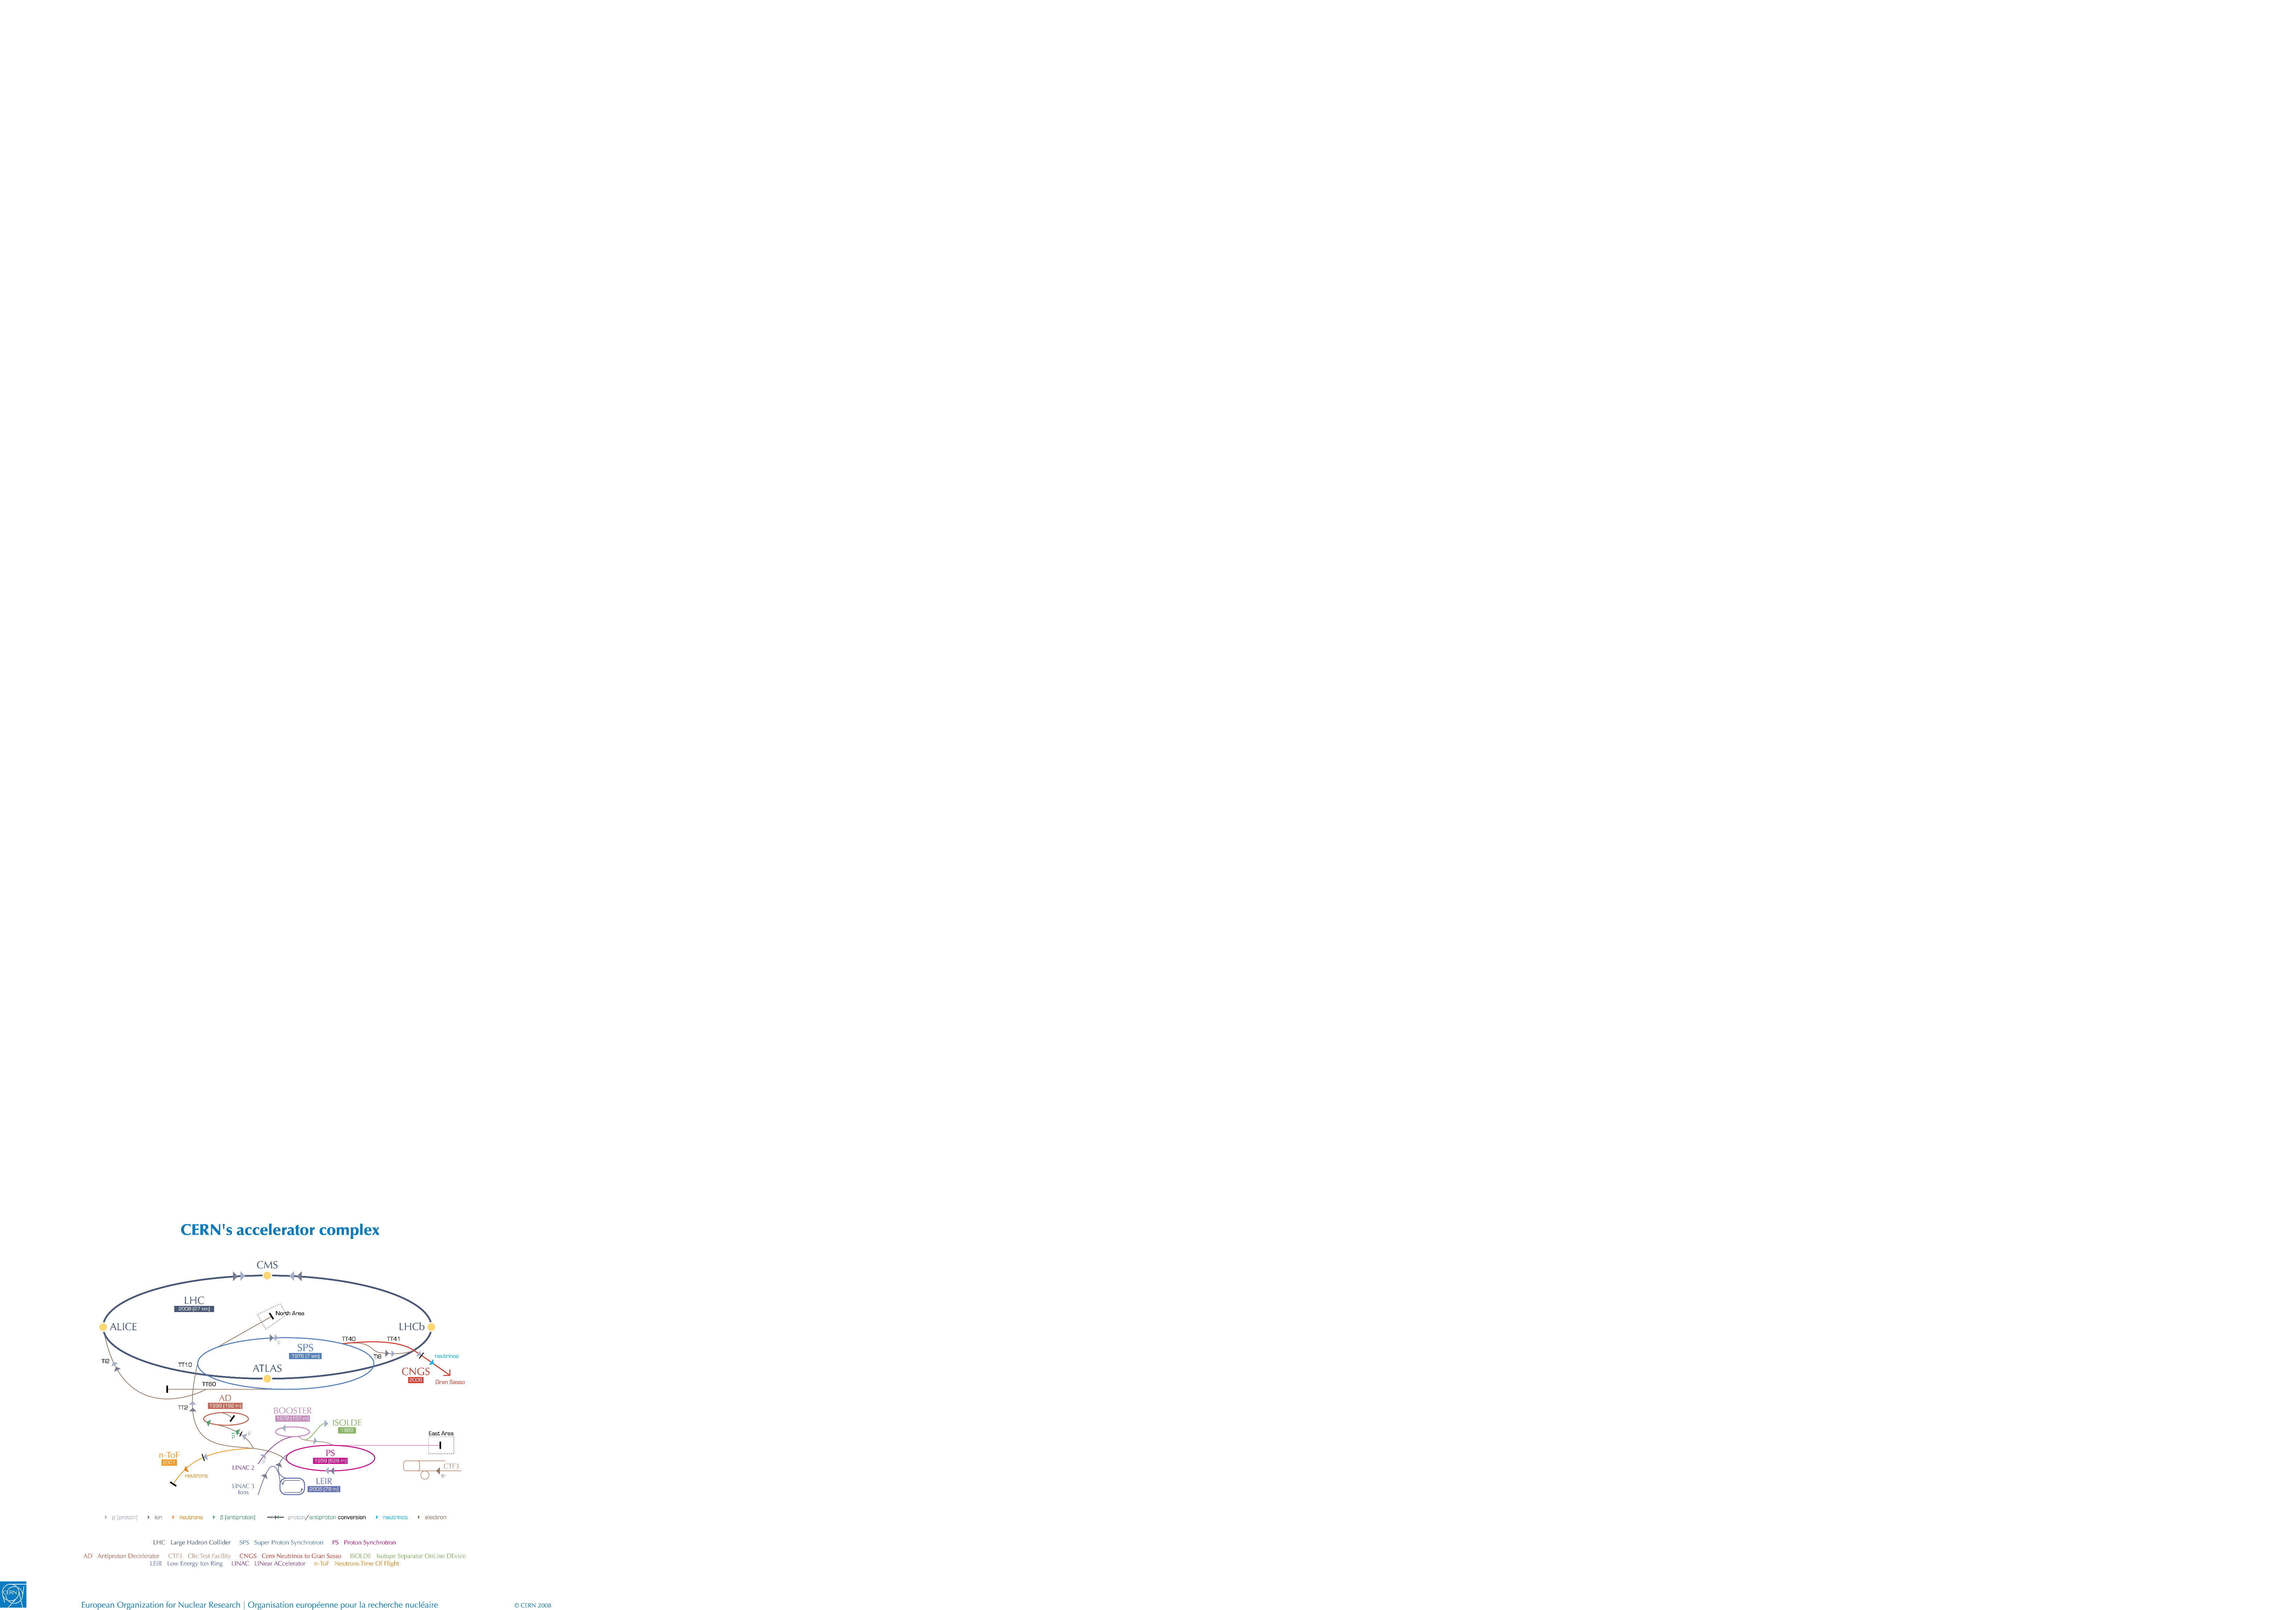
\includegraphics[width=\textwidth]{Images/0812015.pdf}
	\caption{The CERN accelerator complex. ISOLDE gets accelerated protons from LINAC 2 and the PS BOOSTER.}
	\label{fig:accelerators}
\end{figure}


\subsection{Beam production}
A continuous flow of accelerated proton beam bunches from the PSB comes into the ISOLDE facility and collide with a thick production target. The proton beam has an energy of 1.4 GeV and an intensity up to 2 $\mu$A. Two proton beam bunches is separated by 1.2 s \cite{TIF, TIF2013}. ISOLDE typically takes 50\% \cite{MB-spect} of all proton bunches form the PSB, the rest goes to the LHC and other experiments shown in \autoref{fig:accelerators}. In the reaction between the proton beam and the production target, radioactive nuclides are produced in spallation, fission or fragmentation reactions (basically smashing the target into pieces) \cite{ISOLDE-web}. The production target is chosen from a stable region heavier than the nucleus of interest. In our experiment, a production target of tantalum (Ta) was used, producing the elements in the chart of nuclides up to tantalum. A large amount of different isotopes is produced in this way, and the challenge is to extract the nucleus of interest. To obtain the nucleus of interest, we first have to use a method of selecting the atom of interest, and then the nucleus of interest. 

To get the atomic element of interest, one idea is to use a method of selective ionization and then a high voltage electrostatic field to extract the ions. Electronic transitions are characteristic for each chemical element. A laser with precisely tuned wavelength can obtain the photon energy that matches the electronic transition energies in the atom \cite{RILIS-web, RILIS2013}. Thus we can use one laser to excite an electron to a specific excited electron-state in the atom, a second laser to excite electrons further to another excited electron-sate and a third laser to kick out the electron. In this way we only ionize the atomic element of interest. There could be contaminants from surface ionization (atoms that collide with the walls of the ion source), but this is detectable. Using periods of laser on and off, we can detect the resulting contaminants in the beam. The resonance ionization laser ion source (RILIS) is based on the method of step-wise (2-3 step) excitation and ionization of the atom. It is an element-selective process which is used to produce ion beams of the correct element \cite{RILIS}. In this experiment RILIS was used to select Sm with atomic number $Z = 62$. 

At this point we have a continuous beam of Sm ions of 60 keV energy (the target is on a 60 kV high voltage platform) \cite{ISOLDE-web, TIF}. The next step in the process is to have mass separation, and we need to give the continuous beam a fine structure, because the post-accelerator cannot accept a continuous beam coming in, it accelerates bunches. The beam can collide in one of two target stations, either the general purpose separator (GPS) or the high resolution separator (HRS). The GPS has one bending magnet and can deliver beams of different masses ($\pm 13 \%$ of the central beam line mass) simultaneously into three beam lines, while the HRS has two bending magnets with high mass resolving power which delivers the beam into the main (central) beam line \cite{GPS, TIF}. In this experiment the GPS was used to select the isotope of samarium with mass number $A = 140$. 

Now we have a continuous beam of \Sm. The mass separator also gets rid of contaminants that come out of RILIS but have different mass. There could still be isobaric contaminants from surface ionization but luckily there is very little surface ionization for the neighboring elements of Sm. In the radioactive beam experiment trap (REXTRAP) we collect the \Sm\ ions, so that we can release them in bunches that are matched to the fine structure of the linear accelerator (LINAC). REXTRAP is a penning trap which has the tasks of accumulation, bunching and cooling of the RIB \cite{HIE-ISOLDE, REXTRAP1, REXTRAP2}. The ions are released in bunches and transfered to the radioactive beam experiment electron beam ion source (REXEBIS).

REXEBIS is a charge breeder where the RIB is bred to a high charge state \cite{REXEBIS}, with a mass-to-charge ($A/q$) ratio typically between 2.5 and 4.5 \cite{Post-acc}. REXEBIS releases the beam with a certain energy through a mass separator and into the high intensity and energy upgrade of the ISOLDE LINAC (HIE-ISOLDE LINAC) \cite{HIE-ISOLDE}. To accelerate the charged ions (beam) to high energy, we need highly charged ions. The electron beam ion source (EBIS) blasts off more electrons from Sm, which leaves the nucleus in a high charge state, going from \Sm$^{+1}$ to \Sm$^{+34}$ ($A/q \approx 4.1$). The longer the ions stay in REXEBIS, the higher the charge state becomes. We get a distribution of charge states, and we loose those that have the wrong charge state because the LINAC can only accept one charge state \cite{REX-web, HIE-web, EBIS2002, EBIS2010}.

The HIE-ISOLDE LINAC accelerates the beam of \Sm\ to 4.65 MeV/u through the beam line, and magnets bend the beam into Miniball. This experiment was one of the first Miniball experiments with the new upgraded superconducting accelerator.

To have a successful experiment, the purity of the beam is of great importance. Contaminants in the beam can come from different sources  \cite{MB-spect}. From the primary target we can have:
\begin{itemize}
	\item isobaric contaminants which are inseparable by the mass separator because of the same mass number
	\item isotopes with an integer multiple of both mass and charge
\end{itemize}
and from stable isotopes the contaminants can come from:
\begin{itemize}
	\item buffer gas in REXTRAP (e.g. Ne, Ar)
	\item residual gas in REXEBIS (e.g. C, O)
	\item components of REXEBIS (e.g. La from the cathode)
\end{itemize}


\subsection{Target}
\textcolor{red}{Kan skrive om dette i motivasjonen.}


As a target, \Pb\ with a thickness of 1.4 mg/cm$^2$ was chosen. The reason for the choice is that it is very hard to excite \Pb\ since it's doubly magic. We wanted the highest possible $Z ~(= 82)$ of a stable isotope to get maximum excitation probability. 

Since we don't need normalization (because we have the B(E2, $0^+ \rightarrow 2^+$) from the previous experiment \cite{Klintefjord} and from lifetime measurement \cite{BelloGarrote2015}), we have chosen a target that is very hard to excite, so transitions from the target will not complicate the spectrum.

\Pb\ has no quadrupole deformation, the first excited state (2615 keV, $T_{1/2} = 16.7$ ps) is of octupole vibration ($J^\pi = 3^-$). If we are \textcolor{red}{lucky/unlucky?} we might see a little bit of this first excited state in the spectrum. This happens if the "collision" is almost head on, and the target hits one of the inner rings.

Unfortunately there was a finger print on the target, so even before beginning the experiment, we have some contamination (probably carbon). The target wheel is shown in \autoref{fig:TWheel}. 

\begin{figure}[ht]
	\centering
	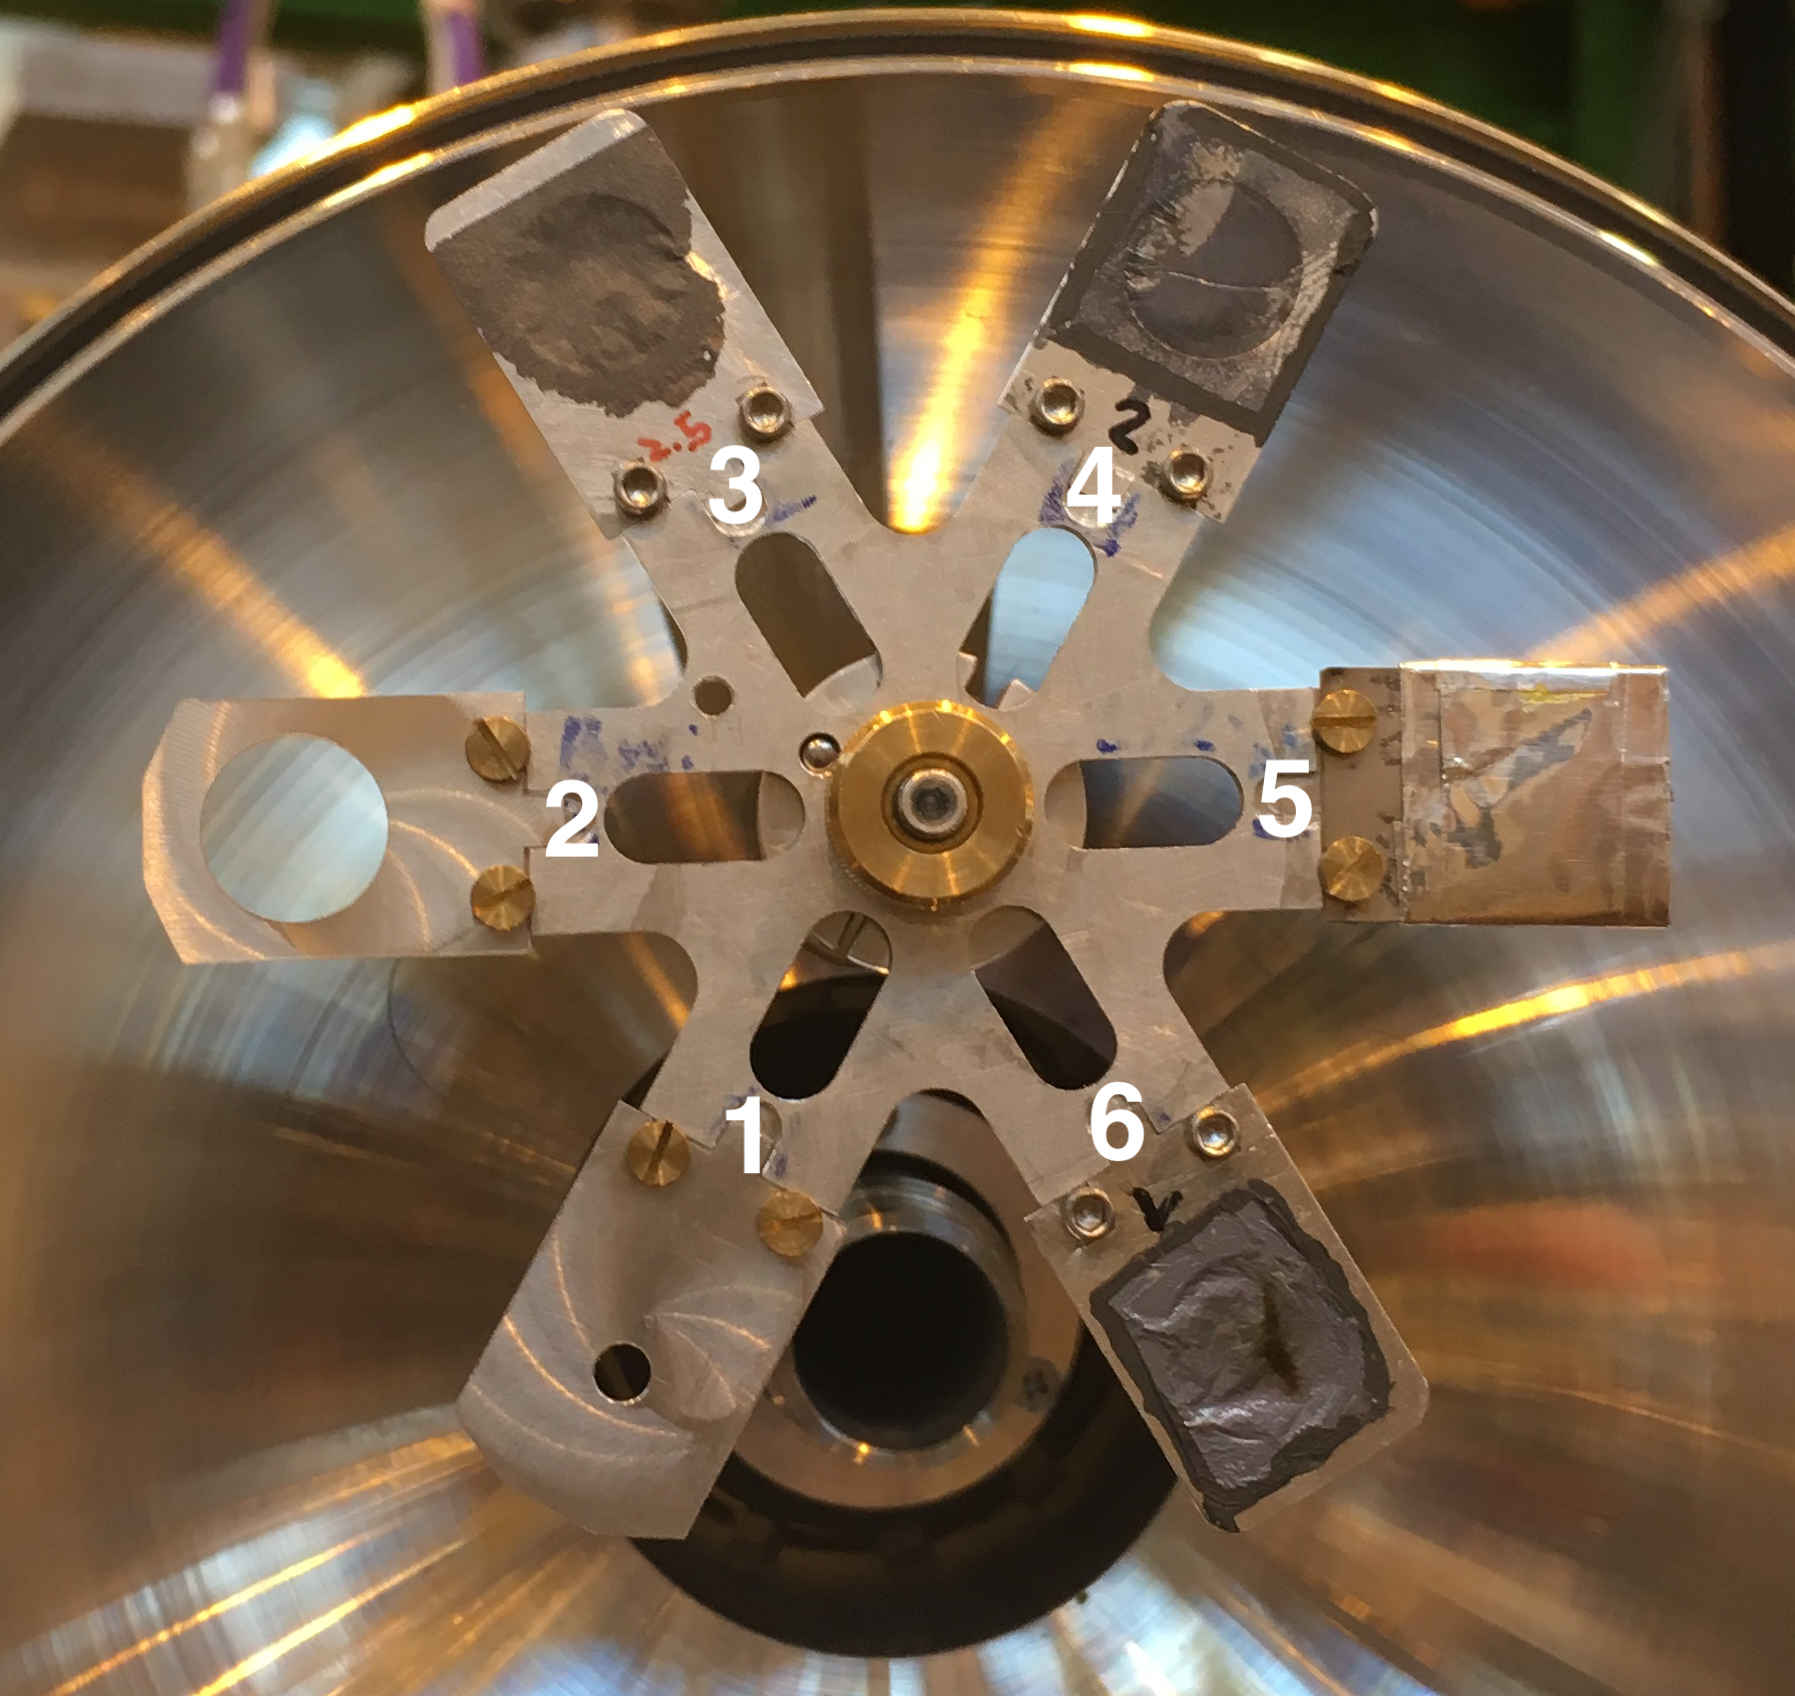
\includegraphics[width=\linewidth]{Images/Target-wheel.png}
	\caption{Target wheel 07.08.2017. Position 6 has the target \Pb\ with thickness 1.4 mg/cm$^2$. Photo by: Liam Gaffney.}
	\label{fig:TWheel}
\end{figure}



\section{Miniball spectrometer}


\begin{figure}[ht]
	\centering
	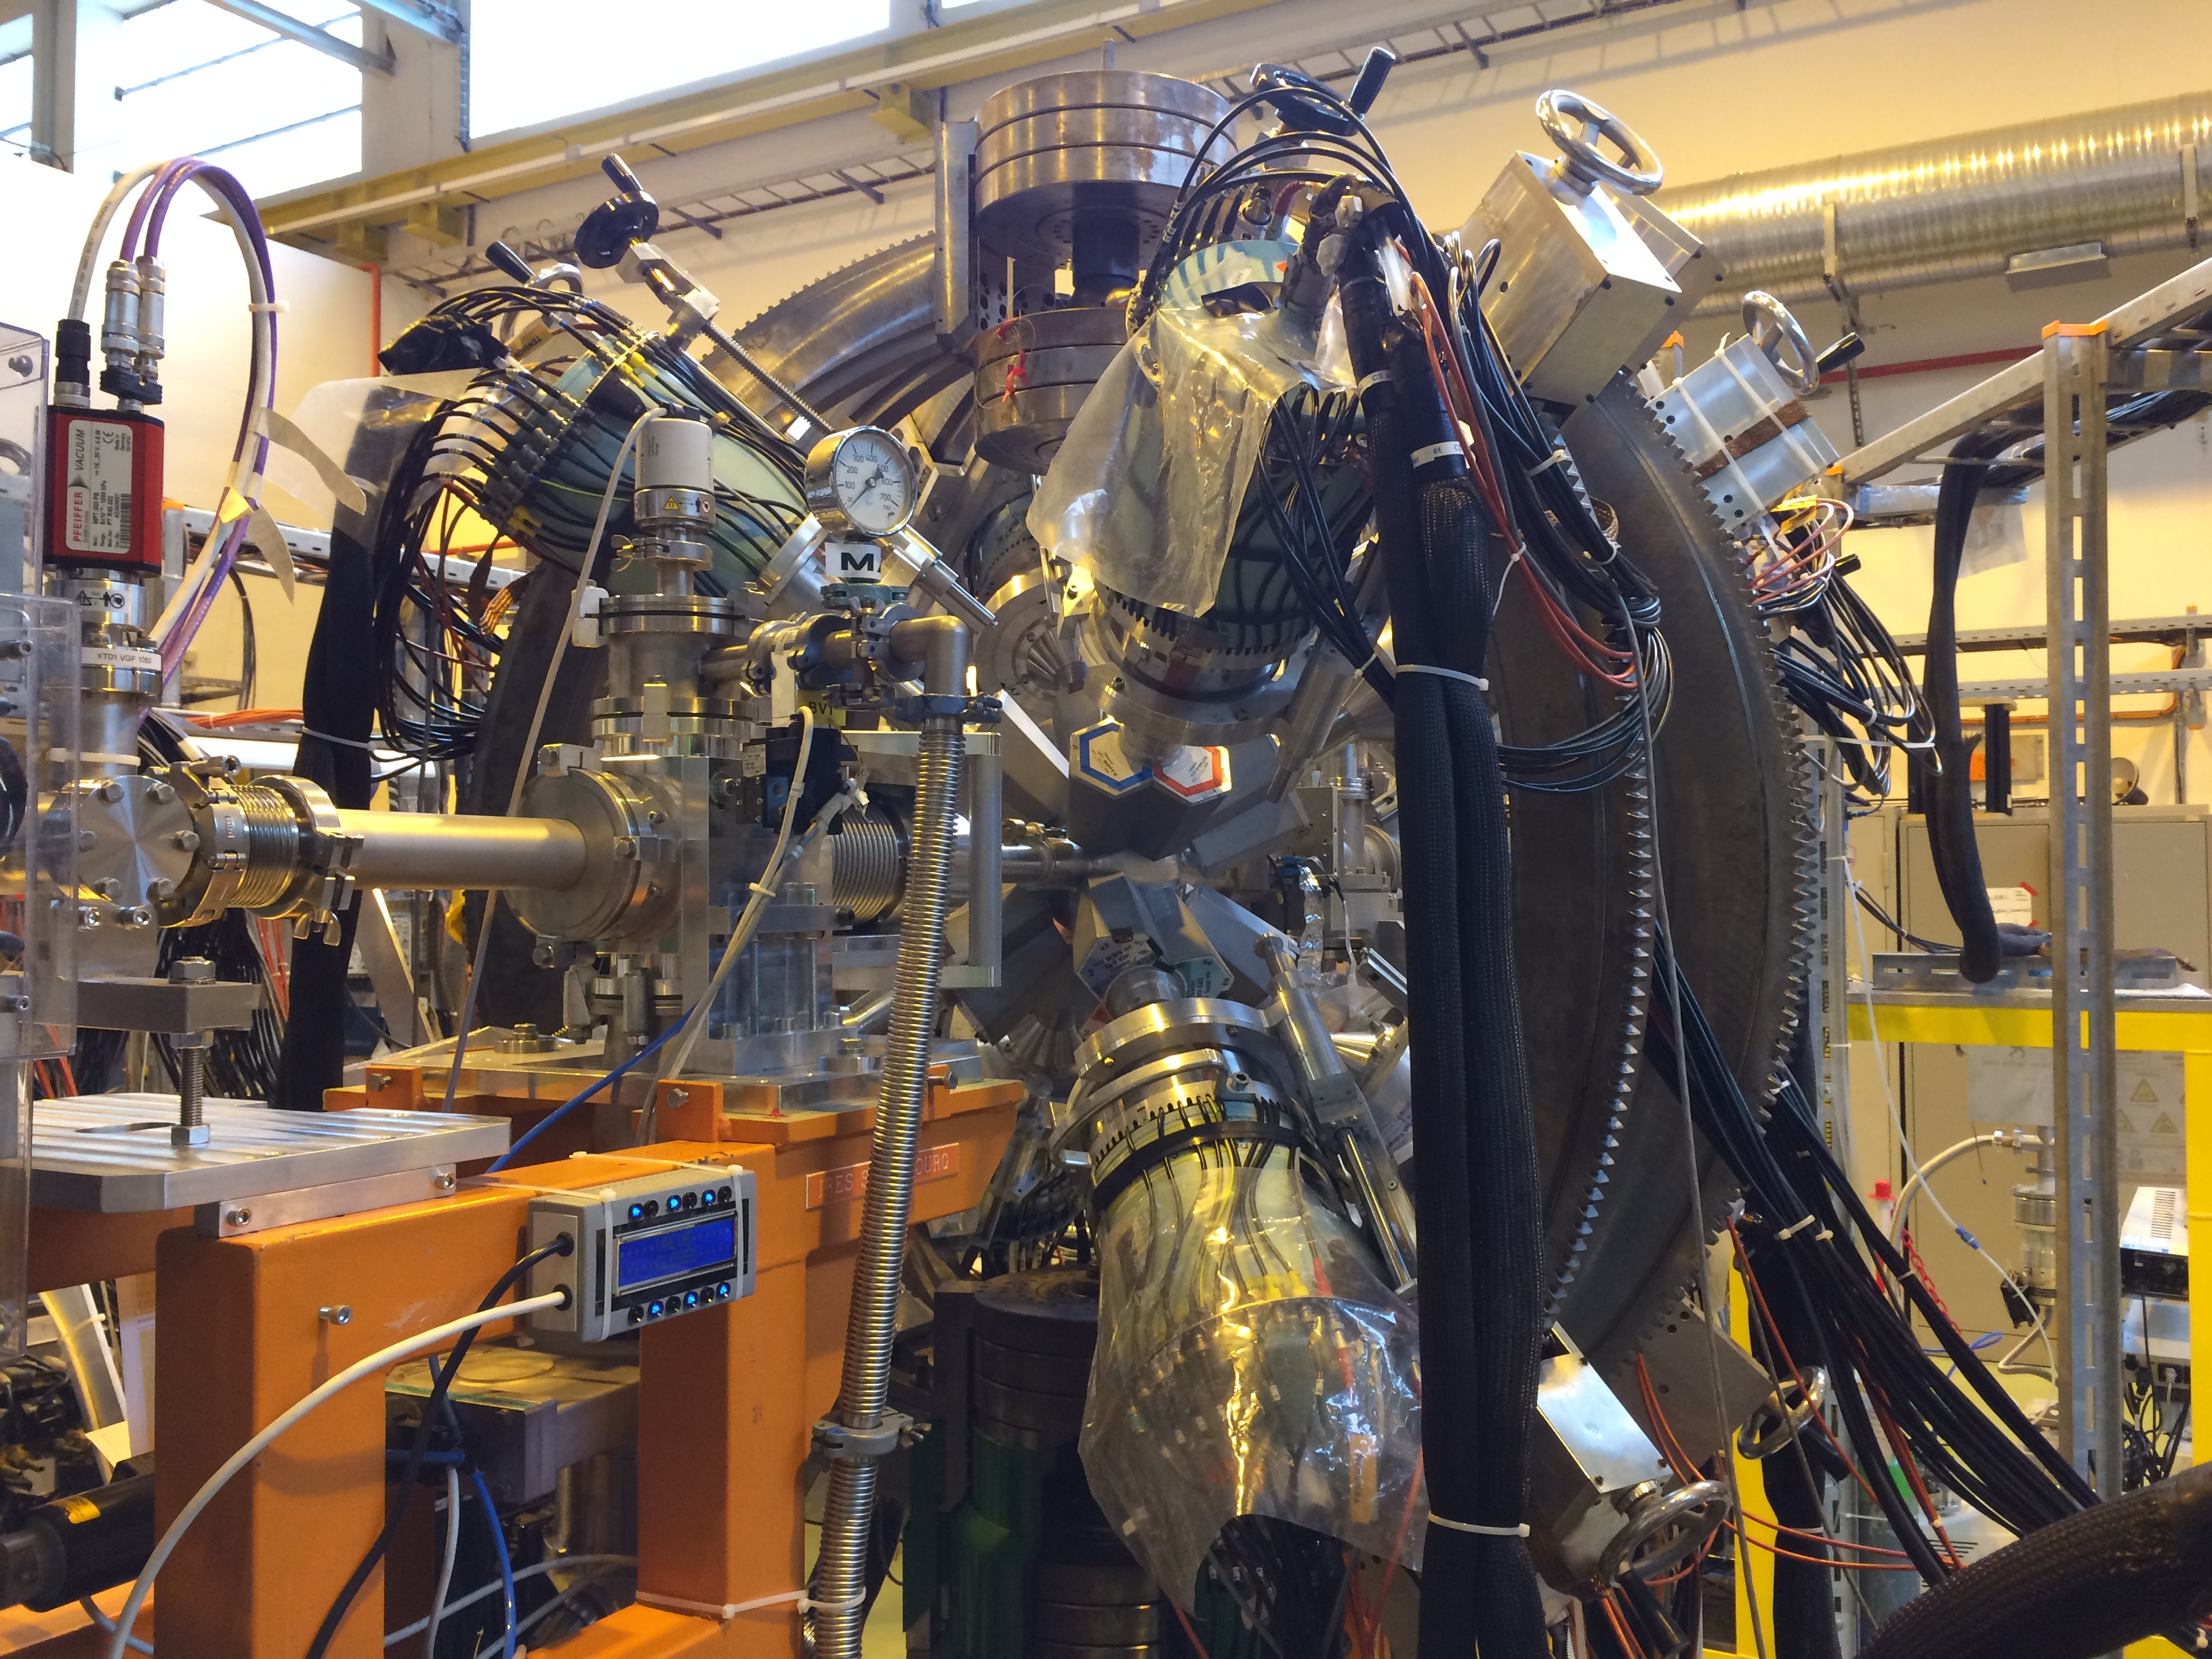
\includegraphics[width=\linewidth]{Images/IMG3849.JPG}
	\caption{Picture of the Miniball spectrometer. Photo by: Trond Wiggo Johansen.}
	\label{fig:MBSpect}
\end{figure}

\begin{figure}[ht]
	\centering
	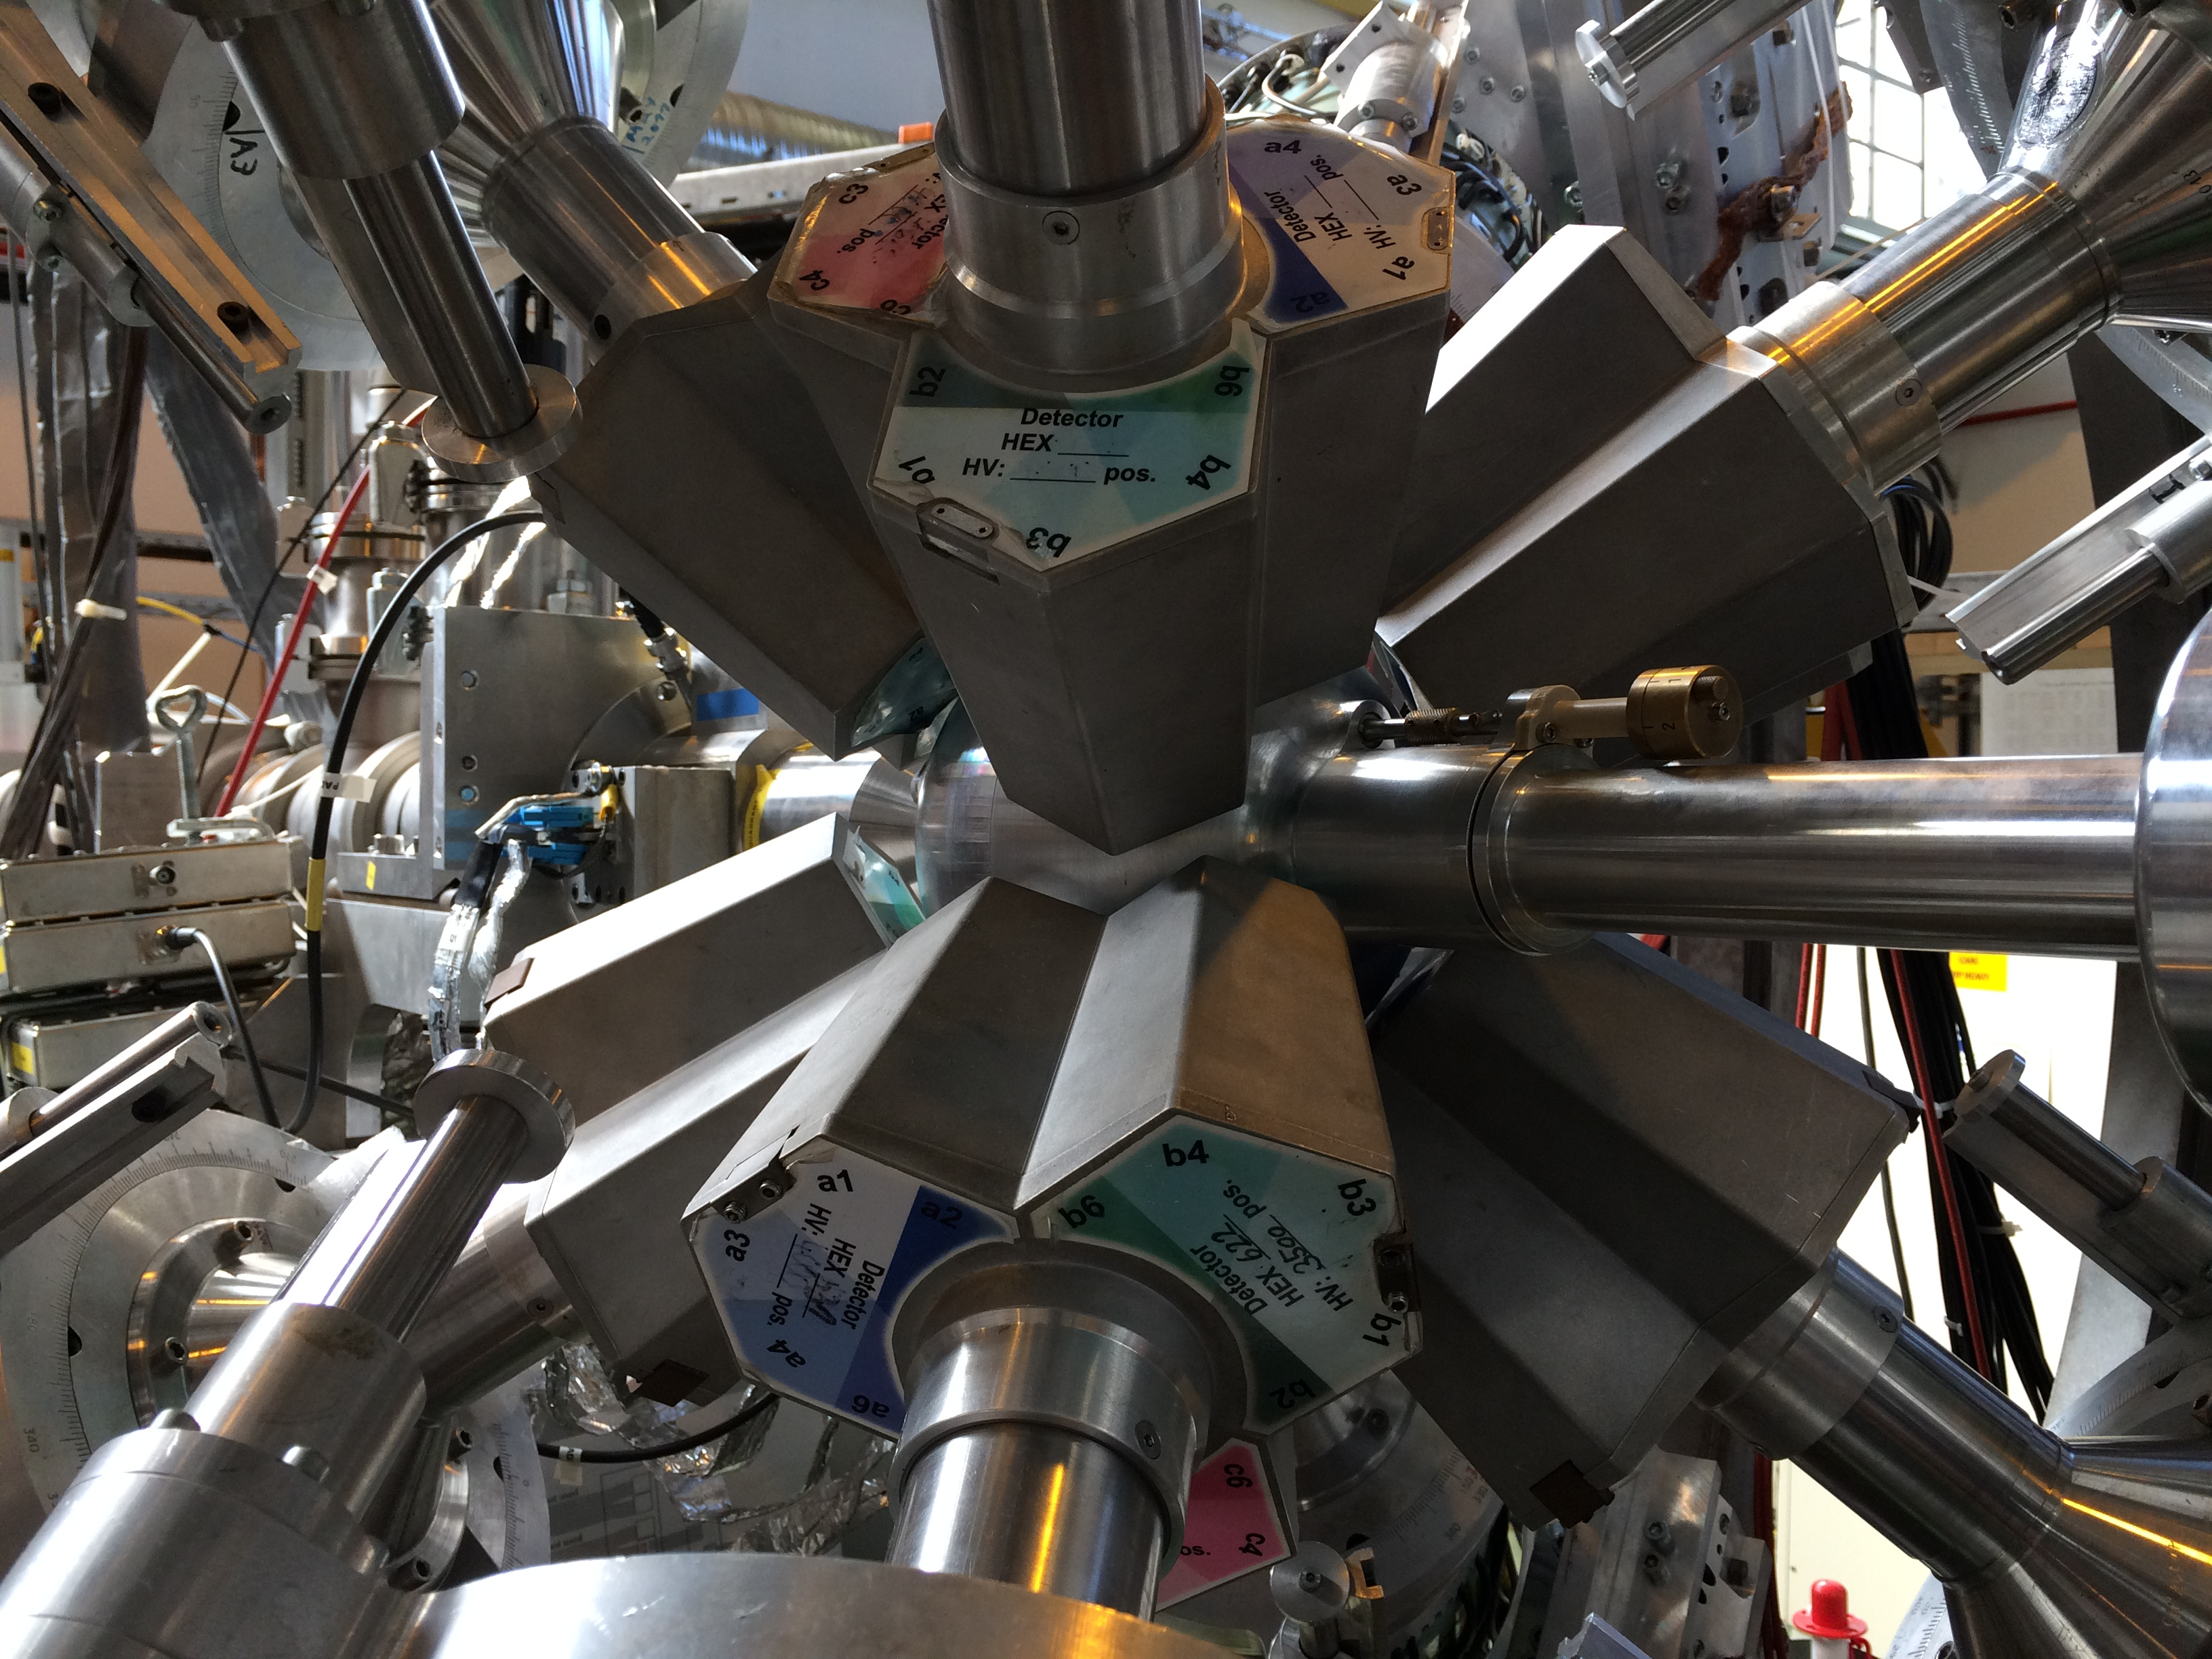
\includegraphics[width=\linewidth]{Images/IMG3917.JPG}
	\caption{Close up picture of the Miniball spectrometer. Photo by: Trond Wiggo Johansen.}
	\label{fig:MBSpectCU}
\end{figure}


\subsection{Particle detector, DSSSD (CD)}
To detect the scattered beam and target nuclei, a segmented double sided silicon strip detector (DSSSD) composed of four quadrants was used. The DSSSD looks very like an audio compact disc (CD), and hence it is called the CD. In the front of the CD, one quadrant consists of 16 annular strips (rings) with a pitch of 2 mm, while the back consists of 24 sector (radial) strips with a pitch of 3.5$^\circ$. The innermost strip has an inner radius of the active area of 9 mm, while the outermost strip has an outer radius of the active area of 40.9 mm. There are in total 160 discrete detector elements for all four quadrants (64 in front, 96 in back). Each quadrant is connected to its own analog to digital converter (ADC). Because of lack of available channels in the ADC, the sector strips in the back are paired up, so that it is effectively 12 sector strips in the back side. The CD detector has a total area of 5000 mm$^2$, where the active area is approximately 93$\%$. The silicon wafer thickness is between 50 $\mu$m and 1000 $\mu$m with a dead layer of 0.3 to 0.8 $\mu$m aluminum (Al) equivalent (\textcolor{red}{what does this mean?}). For simplicity the dead layer thickness is usually assumed to be 0.7 $\mu$m silicon (Si) equivalent (\textcolor{red}{what does this mean?}) \cite{NWarr-CD, MB-spect}. \autoref{tab:CD_spec} shows some of the specifications of the CD and \autoref{fig:CD-FB} shows a sketch of the front and back side. The distance from the target to the CD is 26.98 mm ($\pm$ 1 mm). In the laboratory (LAB) reference frame the CD has a angular coverage between 18.4$^\circ$ and 56.6$^\circ$. \autoref{tab:CD_angles} shows the mid strip CD angles in the laboratory frame for the front of the CD. An extensive description of the CD can be found in \cite{CD-DSSSD}.


\begin{figure}
	\centering
	\begin{subfigure}{\textwidth}
		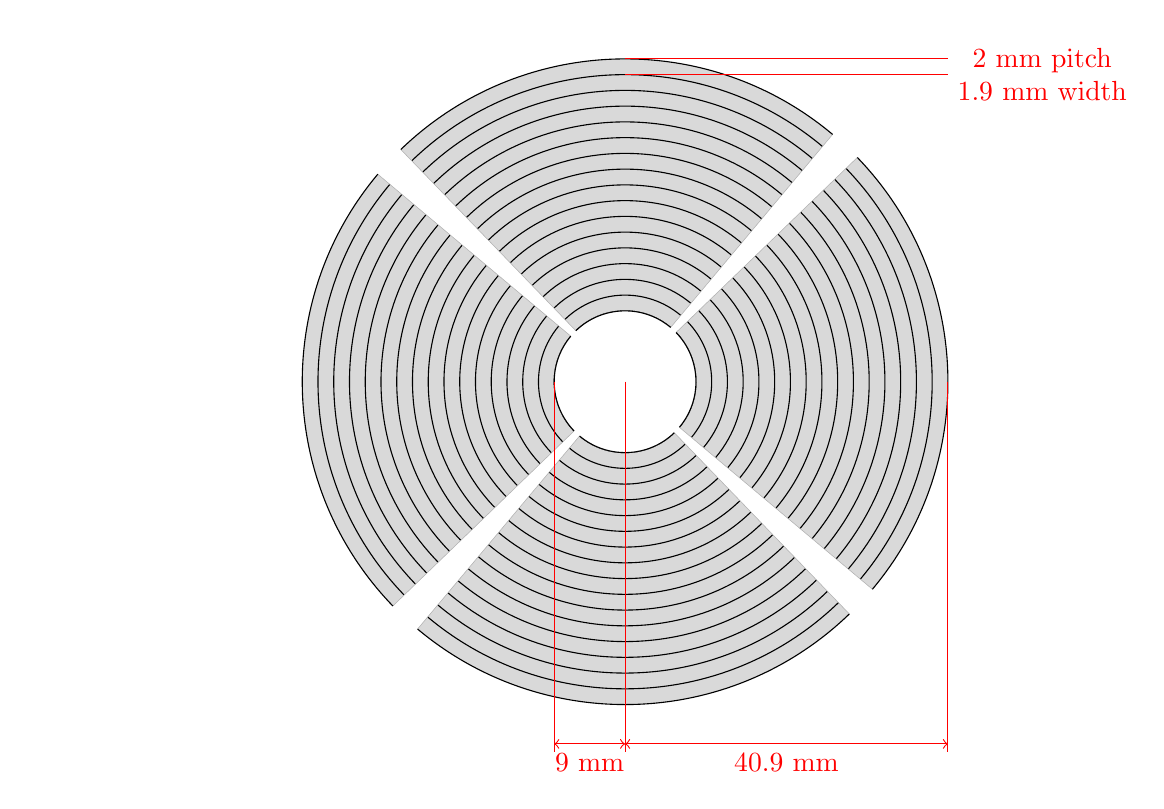
\begin{tikzpicture}
    % Definitions
    \coordinate (origo) at (0,0);
    \def \smallradius{0.9cm}
    \def \bigradius{4.1cm}
    \def \factor{0.2}
    \def \rotation{50}
    %%%
    %%% Front detector
    %%%
    % Gray background
    \foreach \factor in {0, 90, 180, 270} 
    {
        \fill[gray!30, rotate=\factor+\rotation] (origo) -- (\bigradius,0cm) arc (0:84:\bigradius) -- (origo);
    }
    % Annular lines
    \foreach \radius in {0.9, 1.1, ..., 4.1} 
    {
        \draw[black, rotate=\rotation, >=stealth]     (0:\radius) arc (0:84:\radius) {};
        \draw[black, rotate=90+\rotation, >=stealth]  (0:\radius) arc (0:84:\radius) {};
        \draw[black, rotate=180+\rotation, >=stealth] (0:\radius) arc (0:84:\radius) {};
        \draw[black, rotate=270+\rotation, >=stealth] (0:\radius) arc (0:84:\radius) {};
    }
    % Radial quadrant lines
    \foreach \x in {-6, 0, 84, 90, 174, 180, 264, 270} 
    {
        \draw[very thin, black!30, rotate=\rotation] (origo) -- (\x:\bigradius);
    }
    % Inner circle
    \draw[very thin, white, fill=white] (origo) circle (\smallradius);
    % Inner and outer circle arc
    \foreach \factor in {0, 90, 180, 270} 
    {
        \draw[black, rotate=\factor+\rotation, >=stealth] (0:\smallradius) arc (0:84:\smallradius) {};
        \draw[black, rotate=\factor+\rotation, >=stealth] (0:\bigradius) arc (0:84:\bigradius) {};
    }
    % Pitch/width
    \draw[red] (0,\bigradius) -- (\bigradius,\bigradius);
    \draw[red] (0,3.9) -- node[right, pos=1] {\shortstack{2 mm pitch \\ 1.9 mm width}} (\bigradius,3.9);
    % Inner/outer radius
    \draw[red] (-\smallradius,0) -- (-\smallradius,-4.7);
    \draw[red] (origo) -- (0,-4.7);
    \draw[red] (\bigradius, 0) -- (\bigradius,-4.7);
    \draw[<->, red] (-\smallradius,-4.6) -- node[below] {9 mm} (0,-4.6);
    \draw[<->, red] (0,-4.6) -- node[below] {40.9 mm} (\bigradius,-4.6);
    % Vertical alignment with back detector
    \node[] at (-7.47,0) {};
\end{tikzpicture}
		\caption{CD front: The numbering of the strips goes from strip 0 (outermost) to strip 15 (innermost). Quadrants are numbered in clockwise direction with respect to the beam direction, so that left is 1, up is 2, right is 3 and down is 4.}
		\label{fig:CD-F}
	\end{subfigure}
	\begin{subfigure}{\textwidth}
		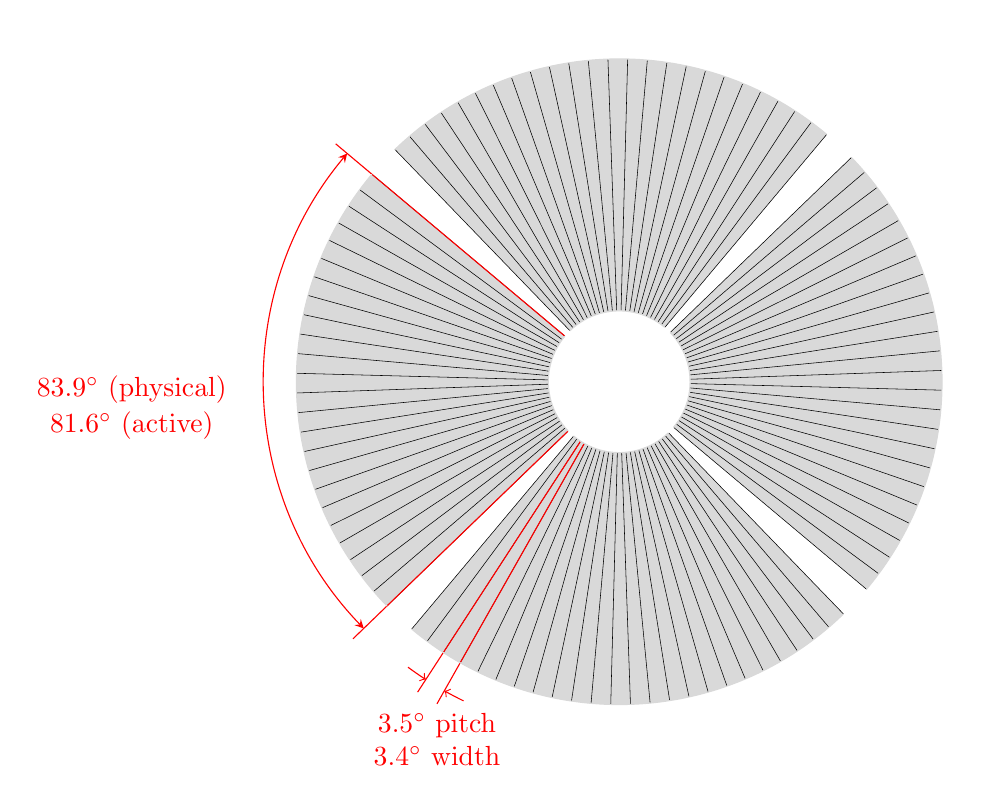
\begin{tikzpicture}
    % Definitions
    \coordinate (origo) at (0,0);
    \def \smallradius{0.9cm}
    \def \bigradius{4.1cm}
    \def \pitch{3.5}
    \def \rotation{50}
    %%%
    %%% Back detector
    %%%
    % Gray background
    \foreach \factor in {0, 90, 180, 270} 
    {
        \fill[gray!30, rotate=\factor+\rotation] (origo) -- (\bigradius,0cm) arc (0:84:\bigradius) -- (origo);
    }
    % Radial lines
    \foreach \x in {0, \pitch, ..., 84} 
    {
        \draw[very thin, black, rotate=\rotation]     (origo) -- (\x:\bigradius);
        \draw[very thin, black, rotate=90+\rotation]  (origo) -- (\x:\bigradius);
        \draw[very thin, black, rotate=180+\rotation] (origo) -- (\x:\bigradius);
        \draw[very thin, black, rotate=270+\rotation] (origo) -- (\x:\bigradius);
    }
    % Physical/active area
    \draw[red, rotate=90+\rotation] (origo) -- (4.7,0);
    \draw[red, rotate=174+\rotation] (origo) -- (4.7,0);
    \draw[<->, red, rotate=90+\rotation, >=stealth] (0:1.1*\bigradius) arc (0:84:1.1*\bigradius) node[anchor=south east, pos=0.7, outer sep=6mm] {\shortstack{$83.9^\circ$ (physical) \\ $81.6^\circ$ (active)}};
    % Pitch/width area
    \draw[red, rotate=187+\rotation] (origo) -- (4.7,0);
    \draw[red, rotate=190.5+\rotation] (origo) -- (4.7,0) node[anchor=north, pos=1] {\shortstack{$3.5^\circ$ pitch \\ $3.4^\circ$ width}};
    \draw[->, red, rotate=183.5+\rotation] (0:1.1*\bigradius) arc (0:\pitch:1.1*\bigradius) {};
    \draw[<-, red, rotate=190.5+\rotation] (0:1.1*\bigradius) arc (0:\pitch:1.1*\bigradius) {};
    % Inner circle
    \draw[very thin, white, fill=white] (origo) circle (\smallradius);
    % Inner and outer circle arc
    \foreach \factor in {0, 90, 180, 270} 
    {
        \draw[gray!30, rotate=\factor+\rotation] (0:\smallradius) arc (0:84:\smallradius) {};
        \draw[gray!30, rotate=\factor+\rotation] (0:\bigradius) arc (0:84:\bigradius) {};
    }
\end{tikzpicture}
		\caption{CD back: The numbering of the strips goes from strip 0 to strip 23 in counter-clockwise direction viewed from this side. Quadrants are numbered in clockwise direction with respect to the beam direction. From this perspective right is 1, up is 2, left is 3 and down is 4.}
		\label{fig:CD-B}
	\end{subfigure}
	\caption{CD sketch, adapted from \cite{NWarr-CD}.}
	\label{fig:CD-FB}
\end{figure}


\begin{table}[ht] 
    \centering 
    \caption{CD specifications.}
	% Data for the CD specification table
\begin{tabular}{lll}
\hline
                            & Annular strips & Secular strips \\
                            & (CD Front)     & (CD Back)      \\
\hline
Number of strips            & 16             & 24             \\
Inner radius of active area &  9.000 mm      & -              \\
Outer radius of active area & 40.900 mm      & -              \\
Strip pitch                 &  2.000 mm      & 3.5$^\circ$    \\
Strip width                 &  1.900 mm      & 3.4$^\circ$    \\
Strip length                &  -             & 31.900 mm      \\
Active angle coverage       & 81.6$^\circ$   & 81.6$^\circ$   \\
Inner strip distance        &  -             & 0.100 mm       \\
\hline
\end{tabular}
	\label{tab:CD_spec}
\end{table}


\begin{table}[ht] 
    \centering 
    \caption{Mid ring CD angles in laboratory frame with distance from target to CD of 26.98 mm. The centroid energy is from simulation with kinsim3. $E_t$ is the energy of the target particle and $E_b$ is the energy of the beam particle.}
	% Data for the CD angles table
\begin{tabular}{ccccc}
\hline
Ring   & \multicolumn{2}{c}{Center of CD ring}                            &             &             \\
number & \shortstack{Distance from \\ beam line [mm]}  & Angle [$^\circ$] & $E_t$ [MeV] & $E_b$ [MeV] \\
\hline
1      & 10                                            & 20.3             & 484.86      & 539.89      \\
2      & 12                                            & 24.0             & 457.53      & 520.55      \\
3      & 14                                            & 27.4             & 428.87      & 499.72      \\
4      & 16                                            & 30.7             & 398.95      & 478.33      \\
5      & 18                                            & 33.7             & 369.54      & 456.71      \\
6      & 20                                            & 36.5             & 340.64      & 435.42      \\
7      & 22                                            & 39.2             & 313.65      & 414.84      \\
8      & 24                                            & 41.6             & 287.31      & 395.31      \\
9      & 26                                            & 43.9             & 262.77      & 376.35      \\
10     & 28                                            & 46.0             & 240.36      & 358.75      \\
11     & 30                                            & 48.0             & 219.53      & 342.40      \\
12     & 32                                            & 49.8             & 198.95      & 326.87      \\
13     & 34                                            & 51.5             & 182.41      & 312.31      \\
14     & 36                                            & 53.1             & 164.55      & 299.11      \\
15     & 38                                            & 54.6             & 151.51      & 286.78      \\
16     & 40                                            & 56.0             & 139.62      & 273.80      \\
\hline
\end{tabular}
	\label{tab:CD_angles}
\end{table}


\subsection{\texorpdfstring{$\gamma$}{Gamma} detectors, high-purity germanium (HPGe)}
The \ga-ray spectrometer consists of a total of 24 six-fold segmented high-purity germanium (HPGe) crystals, which are divided into 8 clusters of 3 crystals each. Each crystal encapsulated and segmented into 6 parts, making a total of 144 segments. For maximum efficiency, the detectors are placed in a compact geometry around the target chamber \cite{NWarr-HPGe, MB-spect}. The detector-array can cover a solid angle of about 60\% of 4$\pi$, when the optimum distance between the target chamber and the HPGe-clusters is achieved. The average energy resolution at $E_\gamma = 1.3$ MeV is 2.3 keV \cite{Butler2017}. 

From each detector we get seven signals in total for each event, one from the core and six from each segment. \textcolor{red}{This requires 168 channels for data aquisition.} The shapes of these signals is analyzed to get information of the position. Because of the segmentation of the detector, a better Doppler correction can be performed compared to using the whole crystal. During operation the HPGe-clusters needs to be cooled by liquid nitrogen and there is an automated filling system in place for this \cite{NWarr-HPGe}. 


\subsection{Target chamber}
p. 10: \newline
\textbf{Target chamber:} \newline
left bottom: \newline
The target chamber used in Coulomb-excitation experiments, surrounded by the eight Miniball clusters is shown in fig. 7(A). It consists of a thin-walled hollow sphere of inner radius $\approx$ 80 mm machined out of a single piece of AlMg$_3$. Inside this chamber a target wheel, that can accommodate six different targets, can be mounted (see fig. 7(B)). The particle detector used for the Coulomb- excitation experiments is shown in fig. 7(C) and will be described in sect. 3. It is positioned 25–31mm from the target wheel (in forward direction) and is mounted on three fixed mounting rods (see fig. 7(B)). There is limited flexibility in the positioning of the detector because of the limited space in the target chamber. \newline
... Each cluster detector resides at an average distance of $\approx$ 10 cm from the center of the target chamber. This spherical configuration ensures a coverage of $\approx$ 60$\%$ of 4$\pi$ around the reaction target (see fig. 7(A)). The angular position of each detector is approximately 45$^\circ$ (for the forward detectors) or 135$^\circ$ (for the backward detectors) with respect to the beam line ($\theta$). In the $\phi$ direction, the four clusters at forward and backward angles are positioned roughly on a circle, separated by 90$^\circ$. \newline

\section{Experimental setup}
\Sm\ Coulomb excitation experiment.


\begin{figure}[ht]
	\centering
	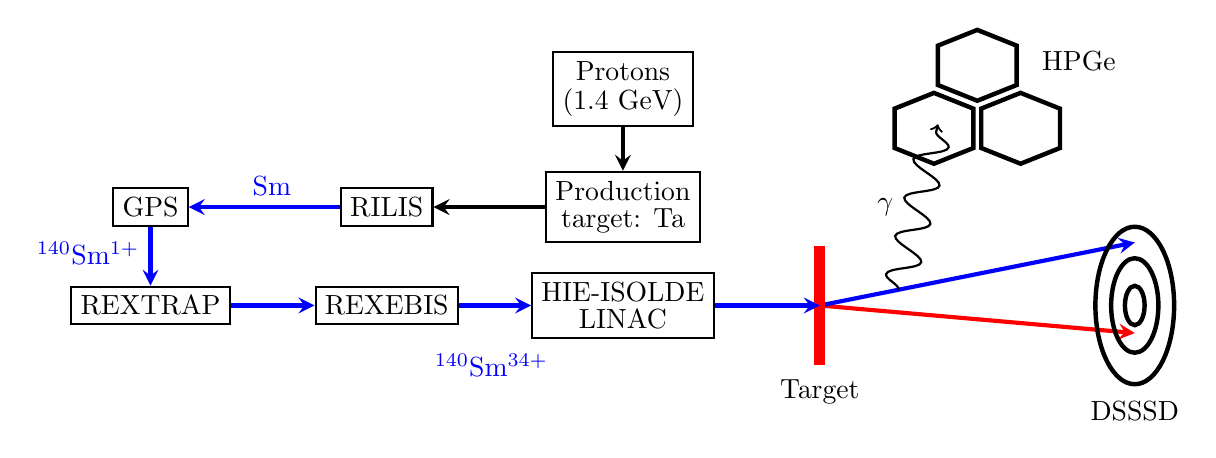
\begin{tikzpicture}
    % Definitions
    \coordinate (origo)   at (0,0);
    \coordinate (Protons) at (-2.5,2.75);
    \coordinate (GPS)     at (-8.5,1.25);
    \coordinate (RILIS)   at (-5.5,1.25);
    \coordinate (PTarget) at (-2.5,1.25);
    \coordinate (REXTRAP) at (-8.5,0);
    \coordinate (REXEBIS) at (-5.5,0);
    \coordinate (HILinac) at (-2.5,0);
    % Target and lines from target
    \draw[->,red,>=stealth,line width=1.5pt] (origo) -- (4,-0.35);
    \draw[->,blue,>=stealth,line width=1.5pt] (origo) -- (4,0.8);
    \draw[red, line width=4pt] (0,0.75) -- (0,-0.75) node[black, below] {Target};
    % Nodes
    \node(P)   at (Protons) [draw,thick] {\shortstack{Protons \\ (1.4 GeV)}};
    \node(G)   at (GPS)     [draw,thick] {GPS};
    \node(R)   at (RILIS)   [draw,thick] {RILIS};
    \node(PT)  at (PTarget) [draw,thick] {\shortstack{Production \\ target: Ta}};
    \node(RXT) at (REXTRAP) [draw,thick] {REXTRAP};
    \node(RXE) at (REXEBIS) [draw,thick] {REXEBIS};
    \node(LIN) at (HILinac) [draw,thick] {\shortstack{HIE-ISOLDE \\ LINAC}};
    % Arrows
    \draw[->,>=stealth,line width=1.5pt]      (P) -- (PT);
    \draw[->,>=stealth,line width=1.5pt]      (PT) -- (R);
    \draw[->,blue,>=stealth,line width=1.5pt] (R) -- (G) node[anchor=south, pos=0.45] {Sm};
    \draw[->,blue,>=stealth,line width=1.5pt] (G) -- (RXT) node[anchor=east, pos=0.45] {$^{140}$Sm$^{1+}$};
    \draw[->,blue,>=stealth,line width=1.5pt] (RXT) -- (RXE);
    \draw[->,blue,>=stealth,line width=1.5pt] (RXE) -- (LIN) node[anchor=north, pos=0.45, outer sep=5mm] {$^{140}$Sm$^{34+}$};
    \draw[->,blue,>=stealth,line width=1.5pt] (LIN) -- (origo);
    % CD 
    \draw[ultra thick] (4,0) ellipse [x radius=0.25cm,y radius=0.125cm, rotate=90];
    \draw[ultra thick] (4,0) ellipse [x radius=0.6cm,y radius=0.3cm, rotate=90];
    \draw[ultra thick] (4,0) ellipse [x radius=1cm,y radius=0.5cm, rotate=90] node[anchor=north, outer sep=11mm] {DSSSD};
    % HPGe
    %\draw (2,2.5) circle (1cm);
    \draw[ultra thick]  (0.95,2) -- ++(0.5,-0.2) -- ++(0.5,0.2) -- ++(0,0.5) -- ++(-0.5,0.2) -- ++(-0.5,-0.2) -- cycle;
    \draw[ultra thick] (1.5,2.8) -- ++(0.5,-0.2) -- ++(0.5,0.2) -- ++(0,0.5) -- ++(-0.5,0.2) -- ++(-0.5,-0.2) -- cycle;
    \draw[ultra thick]  (2.05,2) -- ++(0.5,-0.2) -- ++(0.5,0.2) -- ++(0,0.5) -- ++(-0.5,0.2) -- ++(-0.5,-0.2) -- cycle;
    \node[anchor=west] at (2.7,3.1) {HPGe};
    % Gamma
    \draw[->, decoration={snake,segment length=5mm,amplitude=2mm},decorate,thick] (1,0.2) -- (1.5,2.3) node[left, pos=0.5, outer sep=2mm] {$\gamma$};
\end{tikzpicture}
	\caption{The Coulomb excitation setup at ISOLDE. Adapted from Malin Klintefjord's PhD thesis \cite{Klintefjord}.}
	\label{fig:Coulex}
\end{figure}

\textcolor{red}{From operators logbook: 140Sm34+ at 4.65 MeV/u experiment. A/q = 4.0.}


\begin{figure}[ht]
	\centering
	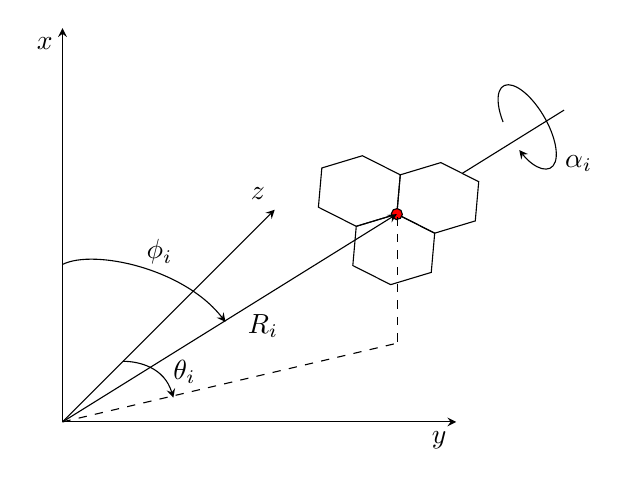
\begin{tikzpicture}
    % Definitions
    \coordinate (origo) at (0,0,0);
    % Coordinate system
    \draw[->,>=stealth] (origo) -- (5,0,0)  node[anchor=north east] {$y$};
    \draw[->,>=stealth] (origo) -- (0,5,0)  node[anchor=north east] {$x$};
    \draw[->,>=stealth] (origo) -- (0,0,-7) node[anchor=south east] {$z$};
    % Line following R
    \draw[>=stealth,rotate=-5] (4,3) -- (6,4.5);
    % HPGe
    \draw[rotate=-5,fill=white] (4,3) -- ++(0.5,-0.2) -- ++(0.5,0.2) -- ++(0,0.5) -- ++(-0.5,0.2) -- ++(-0.5,-0.2) -- cycle;
    \draw[rotate=-5] (3,3) -- ++(0.5,-0.2) -- ++(0.5,0.2) -- ++(0,0.5) -- ++(-0.5,0.2) -- ++(-0.5,-0.2) -- cycle;
    \draw[rotate=-5] (3.5,2.3) -- ++(0.5,-0.2) -- ++(0.5,0.2) -- ++(0,0.5) -- ++(-0.5,0.2) -- ++(-0.5,-0.2) -- cycle;
    % Red point in HPGe center
    \draw[fill=red,rotate=-5] (4,3) circle (2pt);
    % Distance vector
    \draw[->,>=stealth,rotate=-5] (origo) -- (4,3) node[anchor=north,pos=0.6,outer sep=1mm]
    {$R_i$};
    % Vector decomposition
    \draw[dashed] (origo)    -- (4.25,1);
    \draw[dashed] (4.25,2.6) -- (4.25,1);
    % Angles
    \draw[<-,x=0.25cm,y=0.60cm,>=stealth,rotate=30] (27,0.15) arc (-160:160:1 and 1) node[anchor=north west,pos=1.5] {$\alpha_i$};
    \draw[->,>=stealth] (0,0,-2) .. controls (0.2,0,-2) and (0.6,0,-1.8)   .. (1.1,0,-0.8) node[anchor=west,pos=0.6,outer sep=1mm] {$\theta_i$};
    \draw[->,>=stealth] (0,2,0) .. controls (0.4,2.2,0) and (0.7,1.1,-2.2) .. (1.3,0.5,-2) node[above,pos=0.6] {$\phi_i$};
\end{tikzpicture}
	\caption{Miniball angles, where $i$ denotes cluster number from \autoref{tab:Geo}.}
	\label{fig:MB-angles}
\end{figure}


\begin{table}[ht] 
	\centering 
	\caption{Geometry to center Miniball HPGe clusters (red dot) for the Doppler correction.}
	% Data for the Geometry table
\caption{Geometry}
\label{tab:Geo}
\begin{tabular}{ccccc}
\hline
Cluster  &  $\theta$ [$^\circ$]  &  $\phi$ [$^\circ$]  &  $\alpha$ [$^\circ$]  &  R [mm]  \\
\hline
0        &  311.16               &  126.67             &  129.79               &  107.08  \\
1        &  51.08                &  62.74              &  51.83                &  100.59  \\
2        &  309.02               &  126.87             &  51.23                &  105.76  \\
3        &  251.90               &  57.44              &  130.31               &  105.40  \\
4        &  296.93               &  235.53             &  128.74               &  106.48  \\
5        &  233.45               &  239.09             &  46.67                &  105.18  \\
6        &  59.42                &  308.67             &  131.04               &  127.04  \\
7        &  130.56               &  309.09             &  46.46                &  110.18  \\
\hline
\end{tabular}

	\label{tab:Geo}
\end{table}
For Miniball geometry (angles) \cite{NWarr-Angles}. 



%\textcolor{red}{For geometry, see: \url{https://www.ikp.uni-koeln.de/~warr/doc/frame.pdf}}




\begin{table}[ht] 
    \centering 
    \caption{LAB vs CM. Based on LAB input angles from $\theta_b$ and $\theta_t$. From LISE++ kinematics calculator (reaction from the middle of the target).}
	\label{tab:LABvsCM}
    \begin{subtable}{0.45\textwidth}
    		\centering
		\caption{$\theta_b \in [22.0^\circ, 56.7^\circ]$.}
	 	\label{tab:LABvsCM_b}
	 	% Data for the LAB vs CM angle table
\begin{tabular}{ccc}
\hline
\multicolumn{2}{c}{LAB} & CM  \\
$\theta_b$ [$^\circ$]   &  $\theta_t$ [$^\circ$]  &  $\theta_b^{'}$ [$^\circ$]  \\
\hline
22.0                    &  71.7                   &  36.6                       \\
26.0                    &  68.4                   &  43.2                       \\
29.1                    &  65.9                   &  48.2                       \\
32.2                    &  63.4                   &  53.3                       \\
35.2                    &  60.9                   &  58.1                       \\
37.9                    &  58.8                   &  62.4                       \\
40.4                    &  56.8                   &  66.3                       \\
42.8                    &  54.9                   &  70.1                       \\
45.0                    &  53.2                   &  73.5                       \\
47.1                    &  51.6                   &  76.7                       \\
49.0                    &  50.2                   &  79.6                       \\
50.7                    &  48.9                   &  82.1                       \\
52.4                    &  47.6                   &  84.7                       \\
53.9                    &  46.5                   &  86.9                       \\
55.3                    &  45.5                   &  88.9                       \\
56.7                    &  44.5                   &  91.0                       \\
\hline
\end{tabular}
	\end{subtable}
	\begin{subtable}{0.45\textwidth}
		\centering
		\caption{$\theta_t \in [22.0^\circ, 56.7^\circ]$.}
		\label{tab:LABvsCM_t}
		% Data for the LAB vs CM angle table
\begin{tabular}{ccc}
\hline
\multicolumn{2}{c}{LAB} & CM  \\
$\theta_b$ [$^\circ$]   &  $\theta_t$ [$^\circ$]  &  $\theta_b^{'}$ [$^\circ$]  \\
\hline
{\color{red}40.6}  &  {\color{red}56.7}  &  {\color{red}66.6}   \\
{\color{red}42.3}  &  {\color{red}55.3}  &  {\color{red}69.4}   \\
{\color{red}44.2}  &  {\color{red}53.9}  &  {\color{red}72.2}   \\
{\color{red}46.1}  &  {\color{red}52.4}  &  {\color{red}75.2}   \\
{\color{red}48.3}  &  {\color{red}50.7}  &  {\color{red}78.6}   \\
{\color{red}50.6}  &  {\color{red}49.0}  &  {\color{red}82.0}   \\
{\color{red}53.1}  &  {\color{red}47.1}  &  {\color{red}85.8}   \\
{\color{red}56.0}  &  {\color{red}45.0}  &  {\color{red}90.0}   \\
			59.1   &  			  42.8   &  		    94.4    \\
		    62.5   &  			  40.4   &  		    99.2    \\
		    66.1   &  			  37.9   &  		    104.2   \\
		    70.2   &  			  35.2   &  		    109.6   \\
		    75.0   &  			  32.2   &  		    115.6   \\
		    80.2   &  			  29.1   &  		    121.8   \\
		    85.8   &  			  26.0   &  		    128.0   \\
		    93.8   &  			  22.0   &  		    136.0   \\
\hline
\end{tabular}

	\end{subtable}
\end{table}



\bigskip

Experiment code: IS558 

Ta: tantalum (Z = 73)

Sm: samarium (Z = 62)

Pb: lead (Z = 82) \newline



Beam: \Sm\ (T$_{1/2} = 14.82$ min, 4.65 MeV/$u$, total 651 MeV), excellent purity

Target: \Pb\ (Thickness: 1.4 mg/cm$^2$)


Small angle: Forward scattering: Larger distance, weaker \textcolor{red}{EM}-field, less excitation probability.

Large angle: Backward scattering: Closer distance, stronger \textcolor{red}{EM}-field, higher excitation probability. \newline


\bigskip

Expect to measure transition probabilities $B(E2)$ and quadrupole moment (nuclear deformation). 

\bigskip


\begin{figure}
	\centering
	\begin{subfigure}{\textwidth}
		%%
%% Laboratory frame
%%
\begin{tikzpicture}
    % Definitions
    \coordinate (Bleft)  at (-5,0.5);
    \coordinate (Bright) at (5,0.5);
    \coordinate (origo)  at (0,0);
    \coordinate (Tleft)  at (-5,-0.5);
    \coordinate (Tright) at (5,-0.5);
    \coordinate (Bup)    at (2,3);
    \coordinate (Tstart) at (0,-0.5);
    \coordinate (Tdown)  at (1.5,-1.5);
    % Lines
    \draw[dotted] (Tleft) -- (Tright);
    \draw[dotted] (Bleft) -- (Bright);
    \draw[dotted] (origo) -- (Bup);   % particle angle line
    \draw[dotted] (origo) -- (2,-2);  % target angle line
    % Particle paths
    \draw[red,loosely dashed]  (Bleft)  .. controls (-0.5,0.5) and (0.5,0.5) .. (Bup);
    \draw[blue,loosely dashed] (Tstart) .. controls (0.5,-0.5) and (1,-1)    .. (Tdown);
    % Impact parameter
    \draw[<->, >=stealth] (-3,0.5) -- node[left] {b} (-3,-0.5);
    % Center of mass
    \draw[fill=black] (origo) circle[radius=0.07cm] node {};
    \draw[->, >=stealth] (origo) -- (1.5,0) node[right] {$\textbf{V}_{cm}$}; % CM help line
    % Angles
    \draw[->, >=stealth] (1.33,0.5) arc (0:57:1cm)  node[right,pos=0.6,outer sep=1mm] {$\theta_b$};
    \draw[->, >=stealth] (1.5,-0.5) arc (0:-46:1cm) node[right,pos=0.6,outer sep=1mm] {$\theta_t$};
    % Vectors
    \draw[->, >=stealth] (-4.78,0.5) -- ++(1,0)        node[below,pos=0.7,outer sep=0.5mm] {$\textbf{u}$};
    \draw[->, >=stealth] (Bup)       -- ++(0.5,0.75)   node[right,pos=0.4,outer sep=0.6mm] {$\textbf{v}_b$};
    \draw[->, >=stealth] (Tdown)     -- ++(0.66,-0.66) node[right,pos=0.3,outer sep=1.2mm] {$\textbf{v}_t$};
    % Particles
    \draw[draw=blue,fill=blue!20] (Tdown)  circle[radius=0.25cm] node {t};
    \draw[draw=blue,fill=blue!20] (Tstart) circle[radius=0.25cm] node {t};
    \draw[draw=red,fill=red!20]   (Bleft)  circle[radius=0.22cm] node {b};
    \draw[draw=red,fill=red!20]   (Bup)    circle[radius=0.22cm] node {b};
    % Coordinate system 
    \coordinate (CSP) at (-4,1.5);
    \draw[->, >=stealth] (CSP) -- ++(1,0) node[below, pos=0.9] {x};
    \draw[->, >=stealth] (CSP) -- ++(0,1) node[left, pos=0.9]  {y};
    % Vertical alignment with CM frame
    \node[] at (-7.08,0) {};
    % Vertical space from caption text
    \node[] at (0,-2.5) {};
\end{tikzpicture}
		\caption{Laboratory (LAB) frame}
		\label{fig:LAB}
	\end{subfigure}
	\begin{subfigure}{\textwidth}
		%%
%% Center of mass frame
%%
\begin{center}
\begin{tikzpicture}
    % Definitions
    \coordinate (Bleft)  at (-5,0.5);
    \coordinate (Bright) at (5,0.5);
    \coordinate (origo)  at (0,0);
    \coordinate (Tleft)  at (-5,-0.5);
    \coordinate (Tright) at (5,-0.5);
    \coordinate (Bup)    at (2,3);
    \coordinate (Tdown)  at (-2,-3);
    % Lines
    \draw[dotted] (Tleft)  -- (3.75,-0.5);
    \draw[dotted] (Tdown)  -- (Bup);    % 180 degree line
    \draw[dotted] (-0.5,0) -- (1.5,0);  % angle help line
    % Particle paths
    \draw[red,loosely dashed]  (Bleft)  .. controls (-0.5,0.5) and (0.5,0.5)   .. (Bup);
    \draw[blue,loosely dashed] (Tright) .. controls (0.5,-0.5) and (-0.5,-0.5) .. (Tdown);
    % Impact parameter
    \draw[<->, >=stealth] (-3,0.5) -- node[left] {b} (-3,-0.5);
    % Center of mass
    \draw[fill=black] (origo) circle[radius=0.07cm] node {};
    % Angles
    \draw[->, >=stealth] (1,0) arc (0:57:1cm) node[right, pos=0.6, outer sep=1mm] {$\theta_b^{'}$};
    % Vectors
    \draw[->, >=stealth] (-4.78,0.5) -- ++(1,0)        node[below, pos=0.7] {$\textbf{u}^{'}$};
    \draw[->, >=stealth] (4.75,-0.5) -- ++(-1,0)       node[below, pos=0.6] {-$\textbf{u}^{'}$};
    \draw[->, >=stealth] (Bup)       -- ++(0.5,0.75)   node[right, pos=0.4,outer sep=0.5mm] {$\textbf{v}_b^{'}$};
    \draw[->, >=stealth] (Tdown)     -- ++(-0.5,-0.75) node[right, pos=0.8,outer sep=0.5mm] {$\textbf{v}_t^{'}$};
    % Particles
    \draw[draw=blue,fill=blue!20] (Tdown)  circle[radius=0.25cm] node {t};
    \draw[draw=blue,fill=blue!20] (Tright) circle[radius=0.25cm] node {t};
    \draw[draw=red,fill=red!20]   (Bleft)  circle[radius=0.22cm] node {b};
    \draw[draw=red,fill=red!20]   (Bup)    circle[radius=0.22cm] node {b};
    % Coordinate system 
    \coordinate (CSP) at (-4,1.5);
    \draw[->, >=stealth] (CSP) -- ++(1,0) node[below, pos=0.9] {x'};
    \draw[->, >=stealth] (CSP) -- ++(0,1) node[left, pos=0.9] {y'};
    % Vertical space from LAB frame
    \node[] at (0,4.5) {};
\end{tikzpicture}
\end{center}
		\caption{Center of mass (CM) frame.}
		\label{fig:CM}
	\end{subfigure}
	\caption{LAB vs CM frame.}
	\label{fig:LAB-CM}
\end{figure}


\section{Data acquisition system}
Signals from the CD and the HPGe clusters are read out by the ADC and DGF modules and sent to a personal computer (PC) in the data acquisition (DAQ) room at ISOLDE where the data is then stored. The collection of data is done by the \MBOU\ \cite{Maraboou} DAQ system \cite{MB-spect}. It is split in two parts as shown in \autoref{fig:MARaBOOU}, one front-end part based on the multi branch system (MBS) \cite{MBS} and one back-end part based on the ROOT framework \cite{ROOT}. The front-end takes care of data readout, event building and data transportation, while the back-end takes care of the setup, run control, histogramming, data analysis and data storage \cite{MB-spect}.


\textcolor{red}{Other info sources:}
\begin{itemize}
	\item \MBOU\ web page: \url{https://www-old.mll-muenchen.de/marabou/htmldoc/}
	\item \MBOU\ file formatting: \url{https://www-old.mll-muenchen.de/marabou/htmldoc/marabou/IOSpec.html}
\end{itemize}

\begin{figure}[ht]
	\centering
	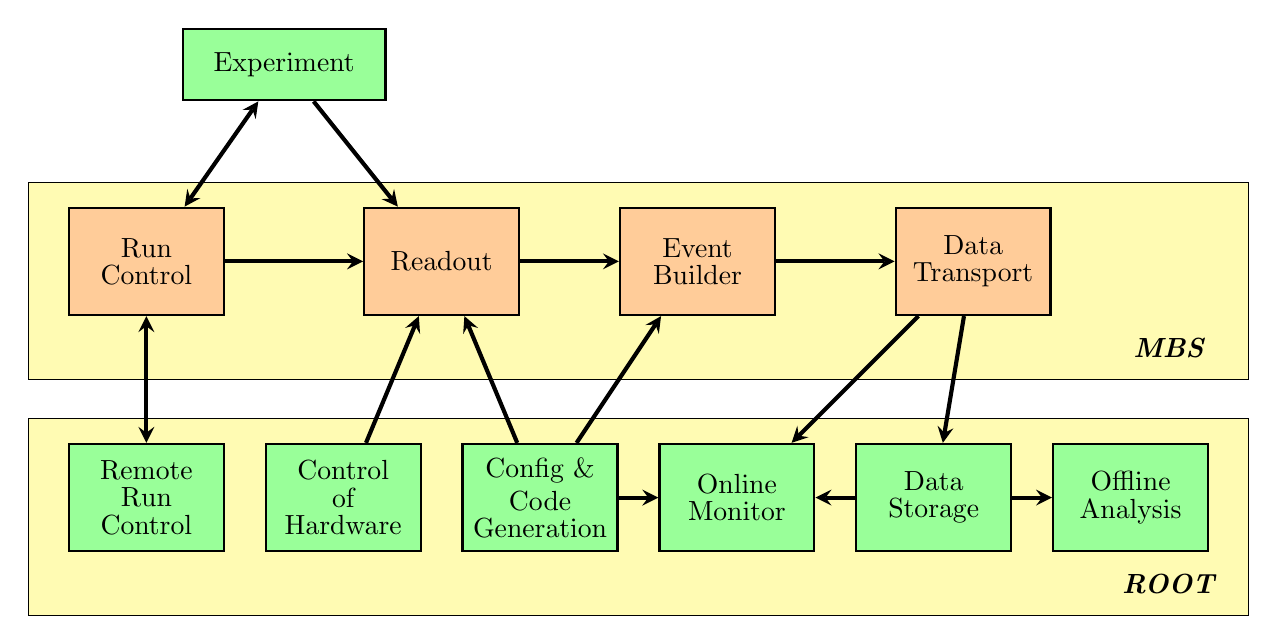
\begin{tikzpicture}
    % Definitions
    \coordinate (EX)  at (1.75,5.5);
    \coordinate (RC)  at (0,3);
    \coordinate (RO)  at (3.75,3);
    \coordinate (EB)  at (7,3);
    \coordinate (DT)  at (10.5,3);
    \coordinate (RRC) at (0,0);
    \coordinate (COH) at (2.5,0);
    \coordinate (CCG) at (5,0);
    \coordinate (OM)  at (7.5,0);
    \coordinate (DS)  at (10,0);
    \coordinate (OA)  at (12.5,0);
    % Rectangles
    \draw[fill=yellow!30] (-1.5,1.5)  rectangle (14,4);
    \draw[fill=yellow!30] (-1.5,-1.5) rectangle (14,1);
    % Nodes
    \node(Expe)   at (EX)  [draw,thick,minimum width=+17ex,minimum height=+6ex,fill=green!40]  {Experiment}; 
    \node(RuCo)   at (RC)  [draw,thick,minimum width=+13ex,minimum height=+9ex,fill=orange!40] {\shortstack{Run \\ Control}};
    \node(ReOu)   at (RO)  [draw,thick,minimum width=+13ex,minimum height=+9ex,fill=orange!40] {Readout};
    \node(EvBu)   at (EB)  [draw,thick,minimum width=+13ex,minimum height=+9ex,fill=orange!40] {\shortstack{Event \\ Builder}};
    \node(DaTr)   at (DT)  [draw,thick,minimum width=+13ex,minimum height=+9ex,fill=orange!40] {\shortstack{Data \\ Transport}};
    \node(ReRuCo) at (RRC) [draw,thick,minimum width=+13ex,minimum height=+9ex,fill=green!40]  {\shortstack{Remote \\ Run \\ Control}};
    \node(CoofHa) at (COH) [draw,thick,minimum width=+13ex,minimum height=+9ex,fill=green!40]  {\shortstack{Control \\ of \\ Hardware}};
    \node(CoCoGe) at (CCG) [draw,thick,minimum width=+13ex,minimum height=+9ex,fill=green!40]  {\shortstack{Config \& \\ Code \\ Generation}};
    \node(OnMo)   at (OM)  [draw,thick,minimum width=+13ex,minimum height=+9ex,fill=green!40]  {\shortstack{Online \\ Monitor}};
    \node(DaSt)   at (DS)  [draw,thick,minimum width=+13ex,minimum height=+9ex,fill=green!40]  {\shortstack{Data \\ Storage}};
    \node(OfAn)   at (OA)  [draw,thick,minimum width=+13ex,minimum height=+9ex,fill=green!40]  {\shortstack{Offline \\ Analysis}};
    \node[thick] at (13,1.9)  {$\textbf{\textit{MBS}}$};
    \node[thick] at (13,-1.1) {$\textbf{\textit{ROOT}}$};
    % Arrows
    \draw[<->,>=stealth,line width=1.5pt] (Expe)   -- (RuCo);
    \draw[->,>=stealth,line width=1.5pt]  (Expe)   -- (ReOu);
    \draw[->,>=stealth,line width=1.5pt]  (RuCo)   -- (ReOu);
    \draw[->,>=stealth,line width=1.5pt]  (ReOu)   -- (EvBu);
    \draw[->,>=stealth,line width=1.5pt]  (EvBu)   -- (DaTr);
    \draw[->,>=stealth,line width=1.5pt]  (DaTr)   -- (OnMo);
    \draw[->,>=stealth,line width=1.5pt]  (DaTr)   -- (DaSt);
    \draw[<->,>=stealth,line width=1.5pt] (RuCo)   -- (ReRuCo);
    \draw[->,>=stealth,line width=1.5pt]  (CoofHa) -- (ReOu);
    \draw[->,>=stealth,line width=1.5pt]  (CoCoGe) -- (ReOu);
    \draw[->,>=stealth,line width=1.5pt]  (CoCoGe) -- (EvBu);
    \draw[->,>=stealth,line width=1.5pt]  (CoCoGe) -- (OnMo);
    \draw[->,>=stealth,line width=1.5pt]  (DaSt)   -- (OnMo);
    \draw[->,>=stealth,line width=1.5pt]  (DaSt)   -- (OfAn);
\end{tikzpicture}
	\caption{\protect\MBOU\ tasks, adapted from \cite{Maraboou}.}
	\label{fig:MARaBOOU}
\end{figure}


% ----------------------------------------------------------------------------------------------------------------------% ----------------------------------------------------------------------------------------------------------------------



\chapter{Data analysis}  

\textcolor{Magenta}{Tilbakemelding: \newline
First: explain the tasks and give the bigger picture of what needs to be done: \newline 
starting point: Raw data in list mode: ID, E, T, ID, E, T, ... (basically) \newline
what you want: Doppler-corrected $\gamma$-spectra with various conditions on particles, angles, etc. \newline
procedure: 3 steps: \newline 
1. convert raw data to ROOT format \newline
2. event-building: \newline
$\bullet$ calibrate detectors, apply thresholds, etc. \newline
$\bullet$ use correlations to build events: particle-$\gamma$ coincidences \newline
$\bullet$ store everything in a tree structure for easy access \newline
3. apply gates on particles and perform Doppler correction \newline
--------- \newline
Could be nice to have a ''cook book'', i.e. step-by-step explanation of this procedure.
}

\bigskip

ROOT: analysere data \cite{ROOT}

kinsim3 \cite{kinsim} + SRIM \cite{SRIM}

MiniballCoulexSort \cite{MBCS}

\bigskip


\begin{table}[H] 
\centering 
\caption{Computer used for data analysis}
\label{tab:PC}
\begin{tabular}{ll}
\hline
Model & MacBook Air (13-inch, 2017) \\
\hline
Processor & 1.8 GHz (Intel Core i5) \\
Memory & 8 GB (1600 MHz DDR3) \\
\hline
\end{tabular}
\end{table}

Run time for sorting data: \newline
TreeBuilder (online calibration): $\sim$ 40-45 min \newline
AQ4Sort (online calibration): $\sim$ 120 min

\begin{table}[H] 
\centering 
\caption{Run time for sorting data.}
\label{tab:run_time}
\begin{tabular}{ll}
\hline
Executable & Run time [min] \\
\hline
TreeBuilder & $\sim$ 45 \\
AQ4Sort & $\sim$ 120 \\
\hline
\end{tabular}
\end{table}

The run time of the bash script was done with the built in script time

\begin{lstlisting}[language=sh]
$ time ./AQ4S.sh Sm online TB
...
real	45m19.265s
user	42m49.653s
sys	0m39.665s
\end{lstlisting}


\begin{lstlisting}[language=sh]
$ time ./AQ4S.sh Sm online Q4
...
real	121m40.830s
user	116m18.361s
sys	1m17.809s
\end{lstlisting}


\begin{lstlisting}[language=sh]
$ time ./AQ4S.sh Sm user TB
...
real	41m11.282s
user	39m45.592s
sys	0m27.777s
\end{lstlisting}


\begin{lstlisting}[language=sh]
$ time ./AQ4S.sh Sm user Q4
...
real	143m47.600s
user	128m6.174s
sys	1m50.921s
\end{lstlisting}

\bigskip

MedToRoot: file 9
% Empty language = plain text
\begin{lstlisting}[language=] 
$ ./M2R.sh Sm
opening file ../../Raw_data/Sm/140Sm_208Pb_pos6_009.med ...
EventBuffer::EventBuffer(GlobalSettings *)
Processing event number       0
Start trigger #14

Processing event number   40000
Stop trigger #15


Unpacked 47268 events:
wrong dgf hit pattern:                      0 ( 0.0 %)
wrong adc headers:                          0 ( 0.0 %)
# of overflows in adc channels:        147009 (311.0 %)
# of underflows in adc channels:            0 ( 0.0 %)
pattern unit mismatches:                    0 ( 0.0 %)

Number of ebis pulses:            23584
Number of t1 pulses:                717
Number of supercycle pulses:        153
committed         351 320 654  bytes to tree tr, 'Tree for on beam data of Coulex setup@Miniball'
and                 4 889 999  bytes to tree bg, 'Tree for on beam background data of Coulex setup@Miniball'
and                68 650 177  bytes to tree tr, 'Tree for off beam data of Coulex setup@Miniball'
wrote                  63 916  bytes to file ../../Raw_data/Sm/140Sm_208Pb_pos6_009_OnBeam.root 	=> compressed by a factor of 5496.6
,                       9 451  bytes to file ../../Raw_data/Sm/140Sm_208Pb_pos6_009_OnBeamBackground.root 	=> compressed by a factor of 517.4
,                      44 809  bytes to file ../../Raw_data/Sm/140Sm_208Pb_pos6_009_OffBeam.root 	=> compressed by a factor of 1532.1
and                    12 904  bytes to file ../../Raw_data/Sm/140Sm_208Pb_pos6_009_Scaler.root 	=> compressed by a factor of 1690.2
\end{lstlisting}


MedToRoot: file 25
\begin{lstlisting}[language=]
$ ./M2R.sh Sm
opening file ../../Raw_data/Sm/140Sm_208Pb_pos6_025.med ...
EventBuffer::EventBuffer(GlobalSettings *)
Processing event number       0
Start trigger #14

Processing event number  100000
Stop trigger #15


Unpacked 105352 events:
wrong dgf hit pattern:                      0 ( 0.0 %)
wrong adc headers:                          0 ( 0.0 %)
# of overflows in adc channels:        535143 (508.0 %)
# of underflows in adc channels:            0 ( 0.0 %)
pattern unit mismatches:                    0 ( 0.0 %)

Number of ebis pulses:            52626
Number of t1 pulses:               1904
Number of supercycle pulses:        150
committed       1  68 292 586  bytes to tree tr, 'Tree for on beam data of Coulex setup@Miniball'
and                12 475  16  bytes to tree bg, 'Tree for on beam background data of Coulex setup@Miniball'
and               213 620 380  bytes to tree tr, 'Tree for off beam data of Coulex setup@Miniball'
wrote                  95 604  bytes to file ../../Raw_data/Sm/140Sm_208Pb_pos6_025_OnBeam.root 	=> compressed by a factor of 11174.1
,                      16 636  bytes to file ../../Raw_data/Sm/140Sm_208Pb_pos6_025_OnBeamBackground.root 	=> compressed by a factor of 749.9
,                      64 319  bytes to file ../../Raw_data/Sm/140Sm_208Pb_pos6_025_OffBeam.root 	=> compressed by a factor of 3321.3
and                    20 646  bytes to file ../../Raw_data/Sm/140Sm_208Pb_pos6_025_Scaler.root 	=> compressed by a factor of 2080.6
\end{lstlisting}

\bigskip

\subsubsection{TreeBuilder}
\begin{lstlisting}[language=]
$ ./Q4S.sh Sm user TB
--- TreeBuilder ---
input file(s):
... <shows a list of all input files>
output file: Sm_user-TreeBuilder-2019-06-20.root
calibration file: ../../Miniball-config/IS558-user.cal
WeightPR: 0.75
Particle distribution:
 Q0 fired: 12243817
 Q1 fired: 12277727
 Q2 fired: 11479362
 Q3 fired: 10936096
Finished.
\end{lstlisting}


\subsubsection{AQ4Sort}
\begin{lstlisting}[language=]
$ ./Q4S.sh Sm user Q4
Info: No flag option for 'AQ4Sort'. Ignoring optional flag.
--- AQ4Sort ---
calibration file: ../../Miniball-config/IS558-user.cal
input file(s):
... <shows a list of all input files>
output file: Sm_user-AQ4Sort-2019-06-24.root
\end{lstlisting}

\subsubsection{CLXAna}
\begin{lstlisting}[language=]
$ ./Coulex.sh -n
--- Coulex: normal ---
Input parameters:
Zb = 62
Ab = 140
Zt = 82
At = 208
Eb = 4650 keV/u
Ex = 531 keV
thick = 1.4 mg/cm2
depth = 0.7 mg/cm2
cddist = 26.98 mm
cdoffset = 242.6 degrees
deadlayer = 0.0007 mm
contaminant = -1 mg/cm2
spededist = 23.6 mm
bg_frac = -0.75
srim = /Users/trondwj/GitHub/MasterThesis/SRIM
cutfile = ../../Sorted_data/outputfile.root:Bcut:Tcut
Begin g_clx loop.
Info in <TCanvas::Print>: pdf file /Users/trondwj/GitHub/MasterThesis/SRIM/140Sm_208Pb.pdf has been created
Info in <TCanvas::Print>: pdf file /Users/trondwj/GitHub/MasterThesis/SRIM/208Pb_208Pb.pdf has been created
Info in <TCanvas::Print>: pdf file /Users/trondwj/GitHub/MasterThesis/SRIM/140Sm_Si.pdf has been created
Info in <TCanvas::Print>: pdf file /Users/trondwj/GitHub/MasterThesis/SRIM/208Pb_Si.pdf has been created
Initialising histograms...
Looping over events...
Warning in <TClass::Init>: no dictionary for class trevts is available
1-particle events = 89020258%)    
Finished.
\end{lstlisting}


\subsubsection{hadd}
After saving "part" from CLXAna-file:
\begin{lstlisting}[language=]
$ cd GitHub/ROOT-framework/build/bin
$ hadd /Users/trondwj/GitHub/MasterThesis/Sorted_data/outputfile.root /Users/trondwj/GitHub/MasterThesis/Sorted_data/part.root /Users/trondwj/GitHub/MasterThesis/Sorted_data/Bcut.root /Users/trondwj/GitHub/MasterThesis/Sorted_data/Tcut.root 
\end{lstlisting}


\subsubsection{•}
\begin{lstlisting}[language=]
\end{lstlisting}


\bigskip

particle-gamma and particle-gamma-gamma coincidence

\textcolor{red}{sjekk opp om energi fra online kalibrering passer med simuleringen.}

\section{Data and sorting}

\subsection{\textcolor{red}{Digital electronics - unnecessary?}}

The Miniball spectrometer \cite{MB-spect} \newline
p. 7: \newline
\textbf{Digital electronics:} \newline
left top: \newline
This means that the FPGA (field programmable gate arrays) can cope with high counting rates with no dead time and is essentially limited only by pile-up. \newline
left bottom: \newline
These buffers contain the energies of the \ga-rays, 48 bit time stamps with 25 ns resolution and either the time to steepest slope or the mirror charge, for each of the 168 channels. This buffer size is large enough that the DGF-4Cs only need to be read out between beam bursts, so the readout does not produce additional dead time. \newline
right top: \newline
ADCs and TDCs are capable of buffering up to 32 events. \newline



Gamma: \\
core ID from 0 to 23 \\
segment ID from 0 to 6 (zero is the core) \\
cluster ID from 0 to 7 \\

ADC: \\
annular (front) strip ID of particle (0 = outer; 15 inner) \\
secular (back) strip ID of particle (0 to 12; clockwise wrt beam) \\

\textcolor{red}{From offl\_root\_med.pdf} \\
"Direction of the central axis of the detector $(r, \theta, \phi)$ and the notation about the axis of the cluster ($\alpha$), \textcolor{red}{is this correct??}. Needed to calculate the positions of the segments or the position of a point determined bye the pulse-shape a analysis.

In order to perform the Doppler shift, we need to know the angle in the Miniball frame of reference of the interaction point. We determine the interaction point either from the segment with the largest energy or using pulse-shape analysis. In the former case, we need to know the position of the centre of each segment. In the latter, we need geometrical information to relate the time-to-steepest slope and ratio of the mirror charge amplitudes to the angle between the interaction point, the target and the emitted particle."





The analysis code for Miniball data is named MiniballCoulexSort and is available on GitHub at \url{https://github.com/Miniball/MiniballCoulexSort}. 
The main steps of how to download, install and use it is outlined in the README.md file in the GitHub repository. 

Data from Miniball comes in the form of .med-files (Miniball Event Data). 
In order to analyze this data in ROOT\footnote{ROOT is a data analysis framework made at CERN.} the first part of the sorting is just to convert the .med-files into .root-files with the script MedToRoot. 

To get useful information out of the converted .root-files, the Treebuilder script is used. 
The .root-file(s) and a calibration file is given to the Treebuilder so it can make event trees that can be used for analyzing the Coulomb excitation events. 

One script that is mentioned in the Miniball GitHub repository, but not showed how to use, is the AQ4Sort. It is used in the same way as the TreeBuilder script, but it sorts the histograms in another way. 
This script is used before and during the calibration of the detectors, because it gives information about every single ring and every single back strip. The one thing to note here, is that the numbering of the detector rings and strips are different from the ones used in Treebuilder. 


The histograms sorted by Treebuilder starts counting from 0 and the AQ4Sort starts counting from 1. 

The ADC spectras from the file sorted by Treebuilder have a naming convention of adc\_q\_s, where $q$ corresponds to the quadrant and $s$ corresponds to the channel. The front energy is saved in adc\_[0-3]\_[0-15] and the back energy from strips 1-12 from all 16 rings (the whole quadrant) is saved in adc\_[0-3]\_[16-27].

\textcolor{Magenta}{Tilbakemelding: \newline 
useful with a table that explains all the different channels and assigns the various detector segments/rings? (naming conventions) (appendix?)
}

\begin{table}[ht] 
	\centering 
	\caption{TreeBuilder vs AQ4Sort.}
	% Data for the TreeBuilder vs AQ4Sort table
\caption{TreeBuilder vs AQ4Sort.}
\label{tab:TBvsAQ4}
\begin{tabular}{cccc}
\hline
Quadrant  &  Front ring or back strip  &  TreeBuilder  &  AQ4Sort      \\
\hline
1         &  Front ring 15             &  adc\_0\_0    &  fE\_Q1\_f1   \\
1         &  Front ring 14             &  adc\_0\_1    &  fE\_Q1\_f2   \\
1         &  Front ring 13             &  adc\_0\_2    &  fE\_Q1\_f3   \\
$\vdots$  &  $\vdots$                  &  $\vdots$     &  $\vdots$     \\
1         &  Front ring 1              &  adc\_0\_14   &  fE\_Q1\_f15  \\
1         &  Front ring 0              &  adc\_0\_15   &  fE\_Q1\_f16  \\
1         &  Back strip 0              &  adc\_0\_16   &  bE\_Q1\_f1   \\
1         &  Back strip 1              &  adc\_0\_17   &  bE\_Q1\_f2   \\
1         &  Back strip 2              &  adc\_0\_18   &  bE\_Q1\_f3   \\
$\vdots$  &  $\vdots$                  &  $\vdots$     &  $\vdots$     \\
1         &  Back strip 11             &  adc\_0\_26   &  bE\_Q1\_f11  \\
1         &  Back strip 12             &  adc\_0\_27   &  bE\_Q1\_f12  \\
          &                            &               &               \\
2         &  Front ring 15             &  adc\_1\_0    &  fE\_Q2\_f1   \\
$\vdots$  &  $\vdots$                  &  $\vdots$     &  $\vdots$     \\
2         &  Front ring 0              &  adc\_1\_15   &  fE\_Q2\_f16  \\
2         &  Back strip 0              &  adc\_1\_16   &  bE\_Q2\_f1   \\
$\vdots$  &  $\vdots$                  &  $\vdots$     &  $\vdots$     \\
2         &  Back strip 12             &  adc\_1\_27   &  bE\_Q2\_f12  \\
          &                            &               &               \\
3         &  Front ring 15             &  adc\_2\_0    &  fE\_Q3\_f1   \\
$\vdots$  &  $\vdots$                  &  $\vdots$     &  $\vdots$     \\
3         &  Front ring 0              &  adc\_2\_15   &  fE\_Q3\_f16  \\
3         &  Back strip 0              &  adc\_2\_16   &  bE\_Q3\_f1   \\
$\vdots$  &  $\vdots$                  &  $\vdots$     &  $\vdots$     \\
3         &  Back strip 12             &  adc\_2\_27   &  bE\_Q3\_f12  \\
          &                            &               &               \\
4         &  Front ring 15             &  adc\_3\_0    &  fE\_Q4\_f1   \\
$\vdots$  &  $\vdots$                  &  $\vdots$     &  $\vdots$     \\
4         &  Front ring 0              &  adc\_3\_15   &  fE\_Q4\_f16  \\
4         &  Back strip 0              &  adc\_3\_16   &  bE\_Q4\_f1   \\
$\vdots$  &  $\vdots$                  &  $\vdots$     &  $\vdots$     \\
4         &  Back strip 12             &  adc\_3\_27   &  bE\_Q4\_f12  \\
\hline
\end{tabular}
	\label{tab:TBvsAQ4}
\end{table}

adc\_0\_0 in the file sorted by Treebuilder is the same as fE\_Q1\_f1 sorted by AQ4Sort. All the front detectors can be found in the Treebuilder-sorted file, but when it comes to the back detector, the single pixels from the strips are not shown. These are available through the AQ4Sort sorted file. For the front detectors the histograms adc\_[0-3]\_[0-15] and fE\_Q[1-4]\_f[1-16] are the same. For the back detectors, we have that adc\_[0-3]\_[16-27] and bE\_Q[1-4]\_b[1-12] are the same. In addition in AQ4Sort we can see the different pixels. The histograms fE\_Q[1-4]\_f[1-16]\_b[1-12] shows the front energy of quadrant 1-4 gated on ring 1-16 and back strip 1-12, while the bE\_Q[1-4]\_f[1-16]\_b[1-12] shows the same, only for the back energy. 

\textcolor{Magenta}{Tilbakemelding: \newline 
a little confusing: is it correct that the treebuilder sort individual spectra for the front and back strips, but if you want coincidences between front and back ($\rightarrow$ pixels) you use AQ4Sort?
}

In the naming convention of adc\_q\_s or fE\_Qu\_fv, where $q \in [0, 1, 2, 3], s \in [0, 1, \ldots, 27]$ and $u \in [1, 2, 3, 4], v \in [1, 2, \ldots, 16]$, the $s = 0$ and $v = 1$ is the outermost ring, while $s = 15$ and $v = 16$ is the innermost ring. In our case, the innermost ring was so destroyed that we have to remove it from the data analysis.


adc\_q\_s, where $q \in [0, 1, 2, 3], s \in [0, 1, \ldots, 27]$.

$p$E\_Q$q$\_f$r$\_b$s$, where $ \in [b, f], q \in [1, 2, 3, 4], r \in [1, 2, \ldots, 16]$ and $s \in [1, 2, \ldots, 12]$. 

The adc\_[0-3]\_[16-27] or bE\_Q[1-4]\_b[1-12] are a combination of all the 16 rings of bE\_Q[1-4]f\_[1, 2, $\ldots$, 16]\_b[1-12].

Don't blame me for the naming convention, I did not write the code. I just tried to make sense of it.


\begin{table}[ht] 
	\centering 
	\caption{ADC}
	% Data for the ADC table
\caption{ADC}
\label{tab:ADC}
\begin{tabular}{cccc}
\hline
ADC    & Quadrant & Channel &  \shortstack{Front ring [F] or \\ back strip [B]} \\
\hline
0 - 3  &  1 - 4   &  0      &  F                    		   					\\
0 - 3  &  1 - 4   &  1      &  F                    		   					\\
0 - 3  &  1 - 4   &  2      &  F                    		   					\\
0 - 3  &  1 - 4   &  3      &  F                    		   					\\
0 - 3  &  1 - 4   &  4      &  F                    		   					\\
0 - 3  &  1 - 4   &  5      &  F                    		   					\\
0 - 3  &  1 - 4   &  6      &  F                    		   					\\
0 - 3  &  1 - 4   &  7      &  F                    		   					\\
0 - 3  &  1 - 4   &  8      &  F                    		   					\\
0 - 3  &  1 - 4   &  9      &  F                    		   					\\
0 - 3  &  1 - 4   &  10     &  F                    		   					\\
0 - 3  &  1 - 4   &  11     &  F                    		   					\\
0 - 3  &  1 - 4   &  12     &  F                    		   					\\
0 - 3  &  1 - 4   &  13     &  F                    		   					\\
0 - 3  &  1 - 4   &  14     &  F                    		   					\\
0 - 3  &  1 - 4   &  15     &  F                    		   					\\
0 - 3  &  1 - 4   &  16     &  B                    		   					\\
0 - 3  &  1 - 4   &  17     &  B                    		   					\\
0 - 3  &  1 - 4   &  18     &  B                    		   					\\
0 - 3  &  1 - 4   &  19     &  B                    		   					\\
0 - 3  &  1 - 4   &  20     &  B                    		   					\\
0 - 3  &  1 - 4   &  21     &  B                    		   					\\
0 - 3  &  1 - 4   &  22     &  B                    		   					\\
0 - 3  &  1 - 4   &  23     &  B                    		   					\\
0 - 3  &  1 - 4   &  24     &  B                    		   					\\
0 - 3  &  1 - 4   &  25     &  B                    		   					\\
0 - 3  &  1 - 4   &  26     &  B                    		   					\\
0 - 3  &  1 - 4   &  27     &  B                    		   					\\
0 - 3  &          &  28     &  Empty                		   					\\
0 - 3  &          &  29     &  Empty                		   					\\
0 - 3  &          &  30     &  Empty                		   					\\
0 - 3  &  1 - 4   &  31     &  PAD                  		   					\\
  4    &          &  0      &  Ionization Chamber   		   					\\
  4    &          &  1      &  Ionization Chamber   		   					\\
\hline
\end{tabular}

	\label{tab:ADC}
\end{table}


\subsection{\textcolor{red}{???}}
The Miniball spectrometer \cite{MB-spect} \newline
p. 8: \newline
\textbf{Efficiency and resolution:}
left bottom: \newline
The application of an add-back (AB) routine involves the summing of the energies of two coincident gamma rays within 100 ns in neighboring cores on the same cluster detector. This situation corresponds to a Compton-scattered \ga-ray event where the energy of the \ga-ray is shared between two or more crystals in the same triple cluster detector. For higher-energy \ga-rays, where scattering from one crystal into its neighbor is quite likely, this improves the efficiency, but for low-energy \ga-rays, where scattering is less likely, summing effects actually reduce the efficiency. For this reason a cut-off is normally applied and AB is only performed for energies above this threshold. \newline


\section{Helping scripts}
All of my scripts are available in the GitHub repository \url{https://github.com/wiggoen/MasterThesis}.

In order to not copy and paste the sorting command in the terminal for every data file, I made two bash scripts to do this. The script \textbf{M2R.sh} is using MedToRoot to take in as many files as you want, and sort it in one go. The other script is \textbf{AQ4S.sh}, which is using either AQ4Sort or Treebuilder to sort a lot of files in one go. 

\textcolor{Magenta}{Tilbakemelding: \newline 
you should have a list of all the files with comments: in-beam data, calibration, laser on-off, problems, which ones can be used and which can not.
}

I also made other helping scripts to get histograms, do fitting, comparison and calibration. 

My scripts: MultiFit.cpp, MultiPlot.cpp, ++ (python, bash,..)

\textcolor{Magenta}{Tilbakemelding: \newline 
if you try to write this step-by-step cook book, you could introduce your scripts wherever is the right place to use them. 
}


\section{Simulation}
To calibrate the data, we need to know the expected energy of the centroids of the peaks. 
This was done by simulating the experiment in a program called kinsim3. The program is written by Liam Gaffney\footnote{Liam Gaffney is a fellow at ISOLDE, affiliated with MINIBALL.} and the purpose of the program is to simulate the kinematics of the experiment. 
It takes into account the Silicon dead layer. 

kinsim3 generates pdf-files of the stopping powers automatically. 
The rest of the plots are available inside the root-file. 
To get the energy simulation for each ring, the function \textbf{cd\_sim\_plots()} from the script \textbf{MultiPlot.cpp} was used. 

\textcolor{Magenta}{Tilbakemelding: \newline 
what are the ingredients for this simulation? \newline
simple 2-body kinematics: energy of projectile, scattering angle of projectile $\implies$ energy of scattered projectile, \{angle, energy\} of binary partner (target recoil) \newline
Stopping powers (which models?) $\rightarrow$ SRIM \newline
Slowing of the particles in the target and in the dead layer of Si
}

\bigskip


CD to target distance: 26.98 mm.


Simulation done by kinsim3

\begin{figure}[H]\centering
    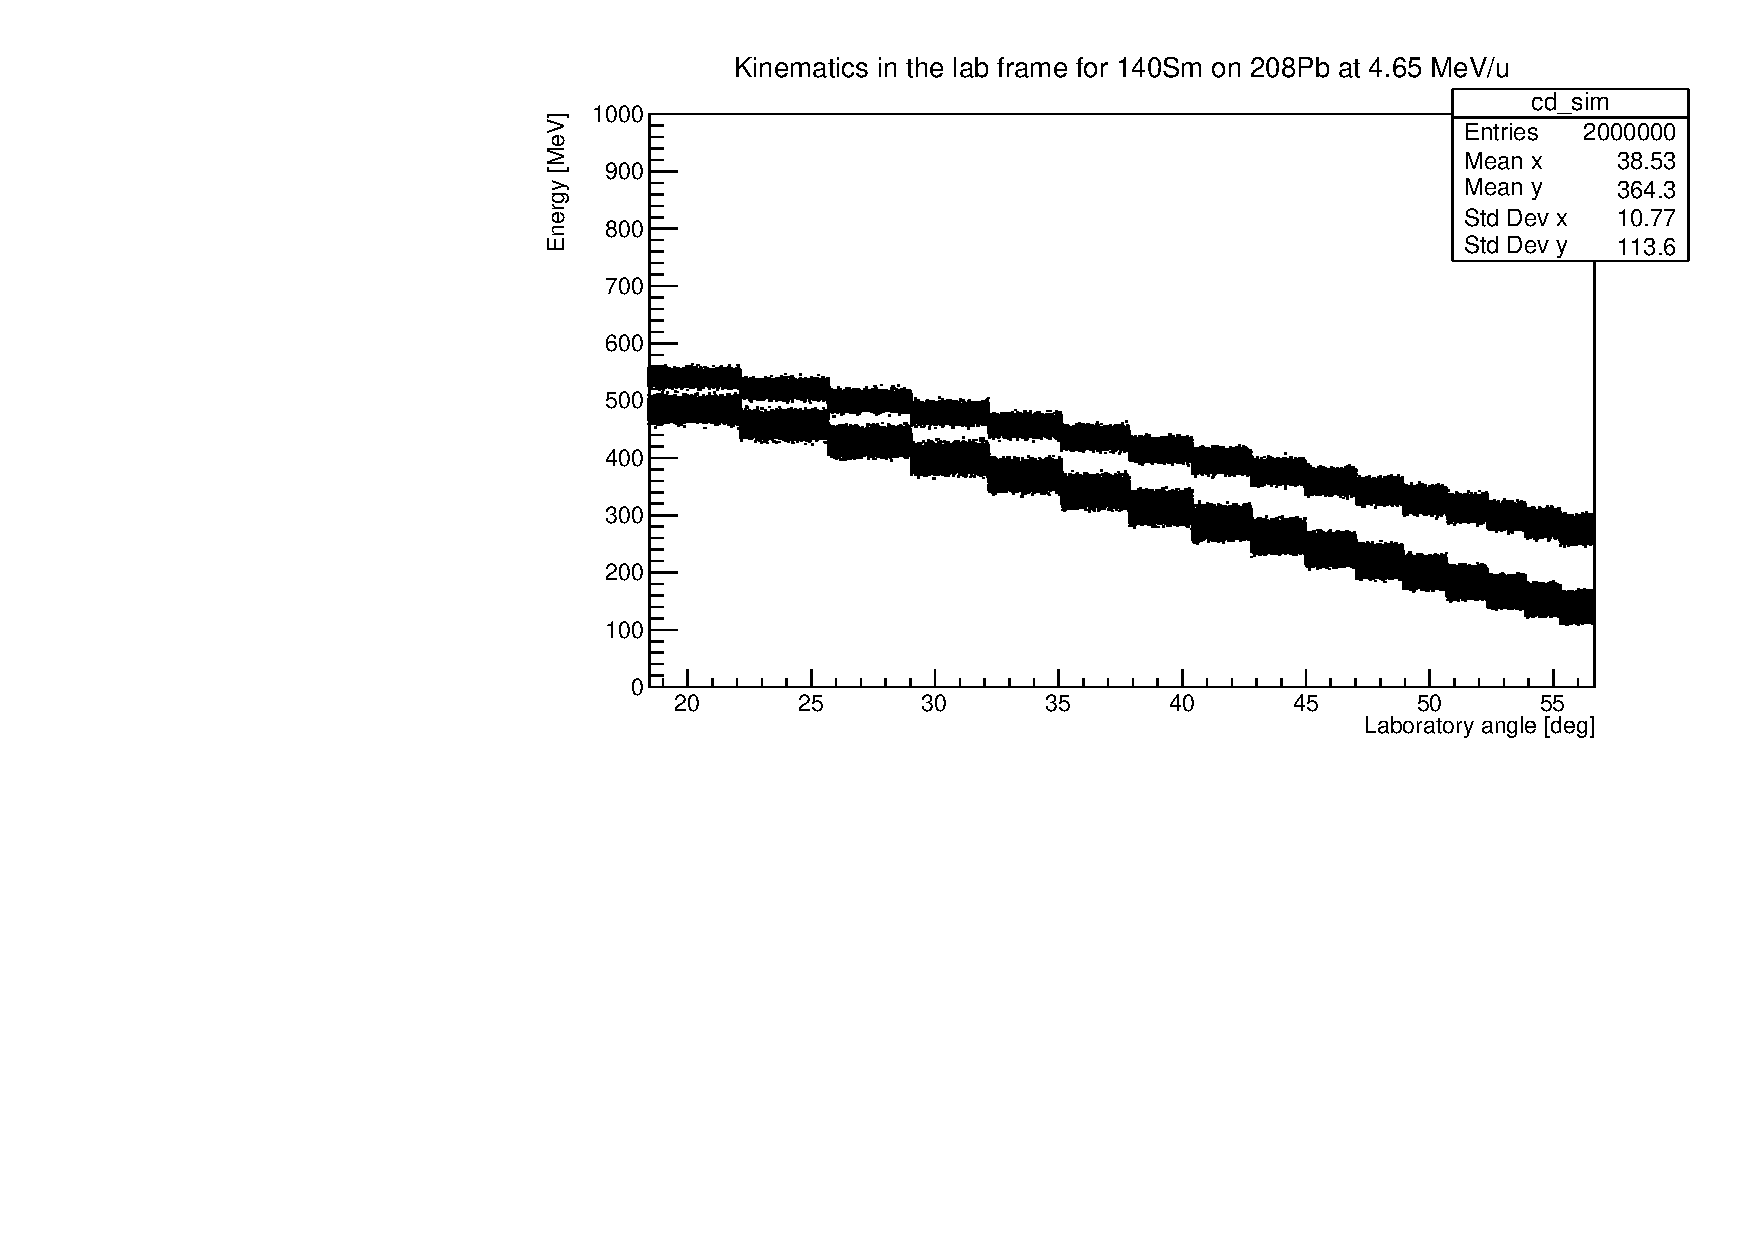
\includegraphics[width=\linewidth]{../Plots/simulation/kin_140Sm_208Pb.pdf}
\end{figure}

\textcolor{Magenta}{Tilbakemelding: \newline 
explain figure: Sm/Pb inner ring, Sm/Pb outer ring \newline
simulation does not consider cross sections: in simulation all angles are equally probable. The corresponding figure from your data looks therefore quite different.
}


\textbf{--- \textcolor{red}{Mail from Liam started} ---} \newline
"the source has a thickness of 1.23 mm, which needs to be factored in so that the CD to target distance is the CD to source distance PLUS the source thickness, i.e. 25.78 mm + 1.23 mm =  27.01 mm. 
This is very close to the 26.98 mm you got from us in August. 
\textcolor{red}{I think that the source data was reanalysed since the original blog entry, giving the 0.03 mm difference!}" \newline
\textbf{--- \textcolor{red}{Mail from Liam ended} ---} \newline


Terminal: Simulation: 140Sm on 208Pb:
\begin{lstlisting}[language=sh]
$ cd GitHub/Miniball/kinsim
$ root
root [0] .L kinsim3.cc+
root [1] kinsim3(62, 82, 140, 208, 1.4, 4.65, 0.02, 1.0, 0.6, 26.98, false, 1e6, "../SRIM")
\end{lstlisting}


kinsim3 function:
\begin{lstlisting}[language=c++]
void kinsim3( int Zb, int Zt, double Ab, double At, double thick /* mg/cm^2 */, double Eb /* MeV/u */,
    double dEb = 0.1 /* MeV/u */, double Ex = 1.0 /* MeV */, double res = 0.6 /* % */,
	double cd_dist = 28.0 /* mm */, bool flat = false /* angular distribution? */,
	long Nevts = 1E6, string srim_dir = "../srim" )
\end{lstlisting}

\bigskip

\textcolor{red}{Say something about SRIM files.}

\bigskip



\section{Calibration}

\textcolor{Magenta}{Tilbakemelding: \newline 
start with explaining the general idea for the calibration: \newline 
determine centroids of peaks in spectra, compare with simulations (kinematics, energy loss) to get linear coefficients (gain + offset). You could show spectra for 2 rings: one where it is ok to get the 2 centroids for Sm and Pb, and one where it is difficult $\rightarrow$ use additional data (Ni?) \newline
Sectors: cover wide angular range $\rightarrow$ no sharp peaks  \newline
Solution: gate on rings to see peaks in sectors and calibrate. \newline
Idea: \newline
1. produce spectra \newline
2. set thresholds: example, explain criteria \newline
3. find calibration coefficients $\rightarrow$ see above \newline
explain strategy, show examples... \newline
4. time calibration 
}


My goal of the calibration was to make a program that could automatically fit the plots i needed, but it became more and more manual labor. 
Because of the shape of the data peaks, it demands very much individual care. 
This I could not do with a automatic program. 
The downfall of the automatic centroid collector came when trying it on the back detectors. 

The total amount particle front detectors to calibrate is 4 quadrants * 16 rings = 64 front detectors 

back detectors: 4 quadrants * 12 strips = 48 back detectors


but to do this, one need all the centroids of the peaks from both sides:

front: 64 detectors * 2 peaks/ring = 128 centroids

back: 48 detectors * 2 peaks/ring * 16 rings =  1536 centroids 

total centroids to collect: 1664 centroids (this I did not want to do manually)

Full calibration with 16 rings and 12 back strips. We had to remove the innermost ring. 



\textcolor{red}{MOVE THE BELOW TO APPENDIX?}

\textcolor{Magenta}{Tilbakemelding: \newline 
up to you. I would do like this: \newline
very technical things about scripts etc. I would move to an appendix. If it helps understanding what you did, I would leave it in the text.
}

For each file converted with MedToRoot, the program makes four files; OffBeam, OnBeam, OnBeamBackground and Scaler. The file we are interested in for analysis is the OnBeam file. 

First all of the interesting files are converted with the M2R.sh script. 
\begin{lstlisting}[language=sh]
$ cd /Users/trondwj/GitHub/MasterThesis/Scripts/sorting 
$ ./M2R.sh Sm
\end{lstlisting}

Then the OnBeam files from M2R.sh is run through using Treebuilder in the AQ4S.sh script. 

\begin{lstlisting}[language=sh]
$ cd /Users/trondwj/GitHub/MasterThesis/Scripts/sorting 
$ ./AQ4S.sh Sm user TB
$ mv Sm_user-TreeBuilder-2019-04-10.root ../../Sorted_data/
\end{lstlisting}


After the sorting, I moved the file to a folder of sorted data, and gave the relative path in the setup\_Sm.txt file in Scripts/plotting/ used as input in the MultiPlot.cpp script. 
Using the MultiPlot.cpp script, the ADC time offsets can be extracted by the following commands
\begin{lstlisting}[language=sh]
$ cd /Users/trondwj/GitHub/MasterThesis/Scripts/plotting
$ root
root [0] .L MultiPlot.cpp++
root [1] check_ADC_time_offsets("setup_Sm.txt")
\end{lstlisting}
or they can be manually reached by
\begin{lstlisting}[language=sh]
$ cd /Users/trondwj/GitHub/MasterThesis/Sorted_data
$ root Sm_user-TreeBuilder-2019-04-10.root
root [1] new TBrowser()
\end{lstlisting}
and in the browser, the histograms named tdiff\_gp\_\textit{i} (where \textit{i} is a number between 0 and 3) will lie under all the folders. The peaks of these plots have the interesting x-value. Zooming into the peaks, it is very clear what value it is. These values are provided in the calibration file under ADC time offsets (ticks). These values can change depending on the amount of data sorted, so it is wise to double check them.

After the peak values have been collected, they should be written into the calibration file
\begin{lstlisting}[language=sh]
# ADC time offsets (ticks)
adc_0.TimeOffset:  0
adc_1.TimeOffset:  -2
adc_2.TimeOffset:  -3
adc_3.TimeOffset:  5
\end{lstlisting}

\begin{figure}[ht]
	\centering
	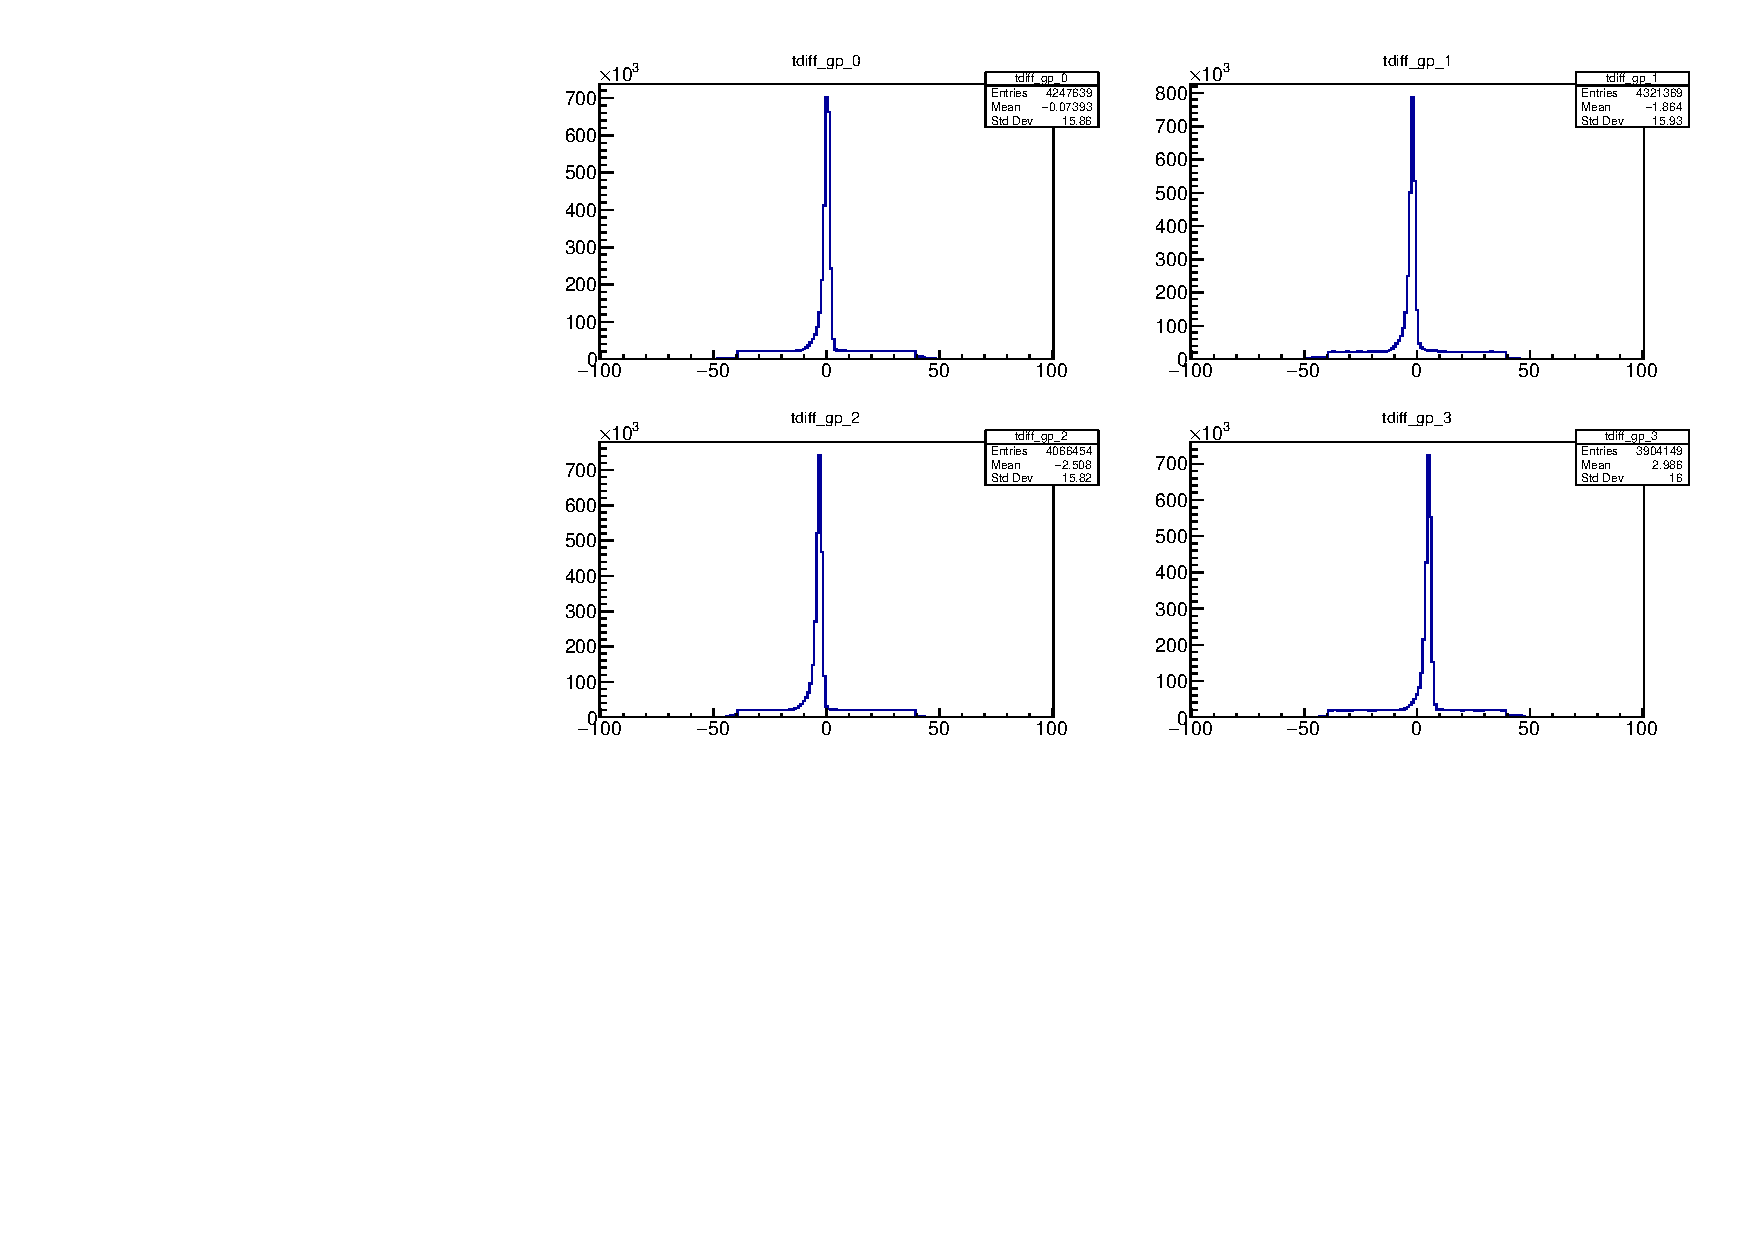
\includegraphics[width=\textwidth]{../Plots/plotting/tdiff_gp_0-3-user.pdf}
	\caption{ADC time offsets.}
	\label{fig:ADC_dt}
\end{figure}

\textcolor{Magenta}{Tilbakemelding: \newline 
one time spectrum per quadrant?
}


\textcolor{red}{HUSK:} Si noe om ADC time offsets + Threshold. Og at man må se på det tidlig, så resortere.


M2R.sh $\rightarrow$ AQ4S.sh$\rightarrow$ check time offset $\rightarrow$ threshold $\rightarrow$ AQ4\_fit() $\rightarrow$ particle-calibration.py $\rightarrow$  ADC\_generator.py $\rightarrow$ copy the calibration from the terminal and paste into calibration file 

\textcolor{Magenta}{Tilbakemelding: \newline 
need to explain the time spectra: start - stop \newline
purpose: align time spectra so that you can set a prompt time gate. \newline
$\rightarrow$ correlate $\gamma$-rays with particles.
}


Simulation fit $\rightarrow$ AQ4\_fit() $\rightarrow$ particle-calibration.py $\rightarrow$  ADC\_generator.py $\rightarrow$ copy the calibration from the terminal and paste into calibration file 

Visualize plots using ROOT and the scripts. 



Skriv om scriptene som er lagd, og at det var litt vanskelig å automatisere kalibreringen. Hvis det skulle vært gjort måtte vi funnet en funksjon med "negatively skewed distribution" or "negative skewness" (right modal), en "left skewed function" (most data is more than the mean). 


I log-skala ser dette mer Gaussisk ut, men det er ikke det i non-log skala. 


Back detector calibration: There are just too much individual differences to calibrate the back detectors with a simple script given a range for all 12 back strips. I found out this way to late. There isn't any range to rule them all, at least since the fitting function can behave very strange given a too small or too big range.



\textbf{--- \textcolor{red}{Mail from Liam begins} ---}

"You might have to investigate the threshold a little bit. The continuum of events at low energy comes from charge sharing between the strips. For these very heavy ions, the total amount of charge deposited gets split between neighbouring strips of the CD. The code does performs some tricks to try and recover the correct energy and position, but that depends on counting the number of strips that fire. Therefore, if the threshold is too low you will include "pedestal" events and it will get things wrong. If the threshold is too high, you will miss some events that have charge sharing and get the wrong energy for your particle. 

The key spectra to look at are "part" and "cd\_debug". The latter counts how many particles have X strips fired on the front side and Y strips fired on the back side.

If you have too many cd\_debug events = 3, then your thresholds are too low. If you have a large continuum/background in the "part" spectrum, your thresholds are too high. Best thing to do is play about with different values.

Bin 20 is when no particle can be found, because there is no energy registered in either the front or the back strips. This can only happen when the front energy is below the software threshold that you set and the back energy is either in a broken strip or is also below the software threshold. Likely it is some noise events or charge sharing that comes below the threshold.

\textcolor{red}{The major problem with the online calibration is that a number of the back strips have the wrong gains}, but it otherwise looks quite good. Have you identified which strips these are, by comparing the gains between the 'online' and 'user' calibrations? You could maybe correct those strips as an intermediate step and see how things look.

the source has a thickness of 1.23 mm, which needs to be factored in so that the CD to target \textcolor{red}{distance is the CD} to source distance PLUS the source thickness, i.e. 25.78 mm + 1.23 mm =  27.01 mm. This is very close to the 26.98 mm you got from us in August. I think that the source data was reanalyzed since the original blog entry, giving the 0.03 mm difference!"

For the centroids, it is very hard to tell in log scale how precise you are with the automatic fitting. I zoomed in on one example (attached) and you can see that the black lines do not really represent the centroid in this instance (black lines too low in energy). Because of the complex peak shapes, it is very hard to do this with automatic fitting it seems. 

It honestly might be better to simply hover your mouse over the correct "feature" of the peak, be it the centroid or the maximum, and compare that. The fitting just doesn't seem reliable.

If you do not have the cdpad option selected, then there will be no particle events, because they come in the CD. The -s flag is for adding particles which come without a gamma-ray and the add back flag is for adding Compton scattered events together in the Miniball clusters. 

What you observe around channel number 20 in the ADC events is the so-called pedestal. There is a single common gate for the each ADC (containing channels from one CD quadrant). Therefore, when there is an event in one strip of the CD all channels are readout,  but the channels without a real event read a "zero" energy. These are the events in the pedestal. You should define your threshold for each ADC channel to be above this peak. You are simply zoomed in to the wrong range. Maybe try with log scale on the y-axis and you will see that there should be a cut off at low-energy. After a correct calibration is applied (as you can see for adc\_1\_19 in your example), this pedestal will be calibrated out of the physical energy range.

The nominal calibration will be quite good for most detectors in a certain energy range, because it is designed to be that way. The gains of each DGF are matched during the setup of the experiment so that the online analysis is more straightforward. However, there are some non-linearities and drifting offsets and gains over time that have to be corrected for with a proper calibration using the 133Ba/152Eu source data. 

\textbf{--- \textcolor{red}{Mail from Liam ended} ---}

\textcolor{Magenta}{Tilbakemelding: \newline 
I presume that charge sharing is only considered if 2 firing strips are neighbors?
}

\textbf{Pedestal}

The pedestal is like a massive statue in front of the interesting data. 


We use a threshold to cut away the pedestal.

\begin{figure}[ht]
	\centering
	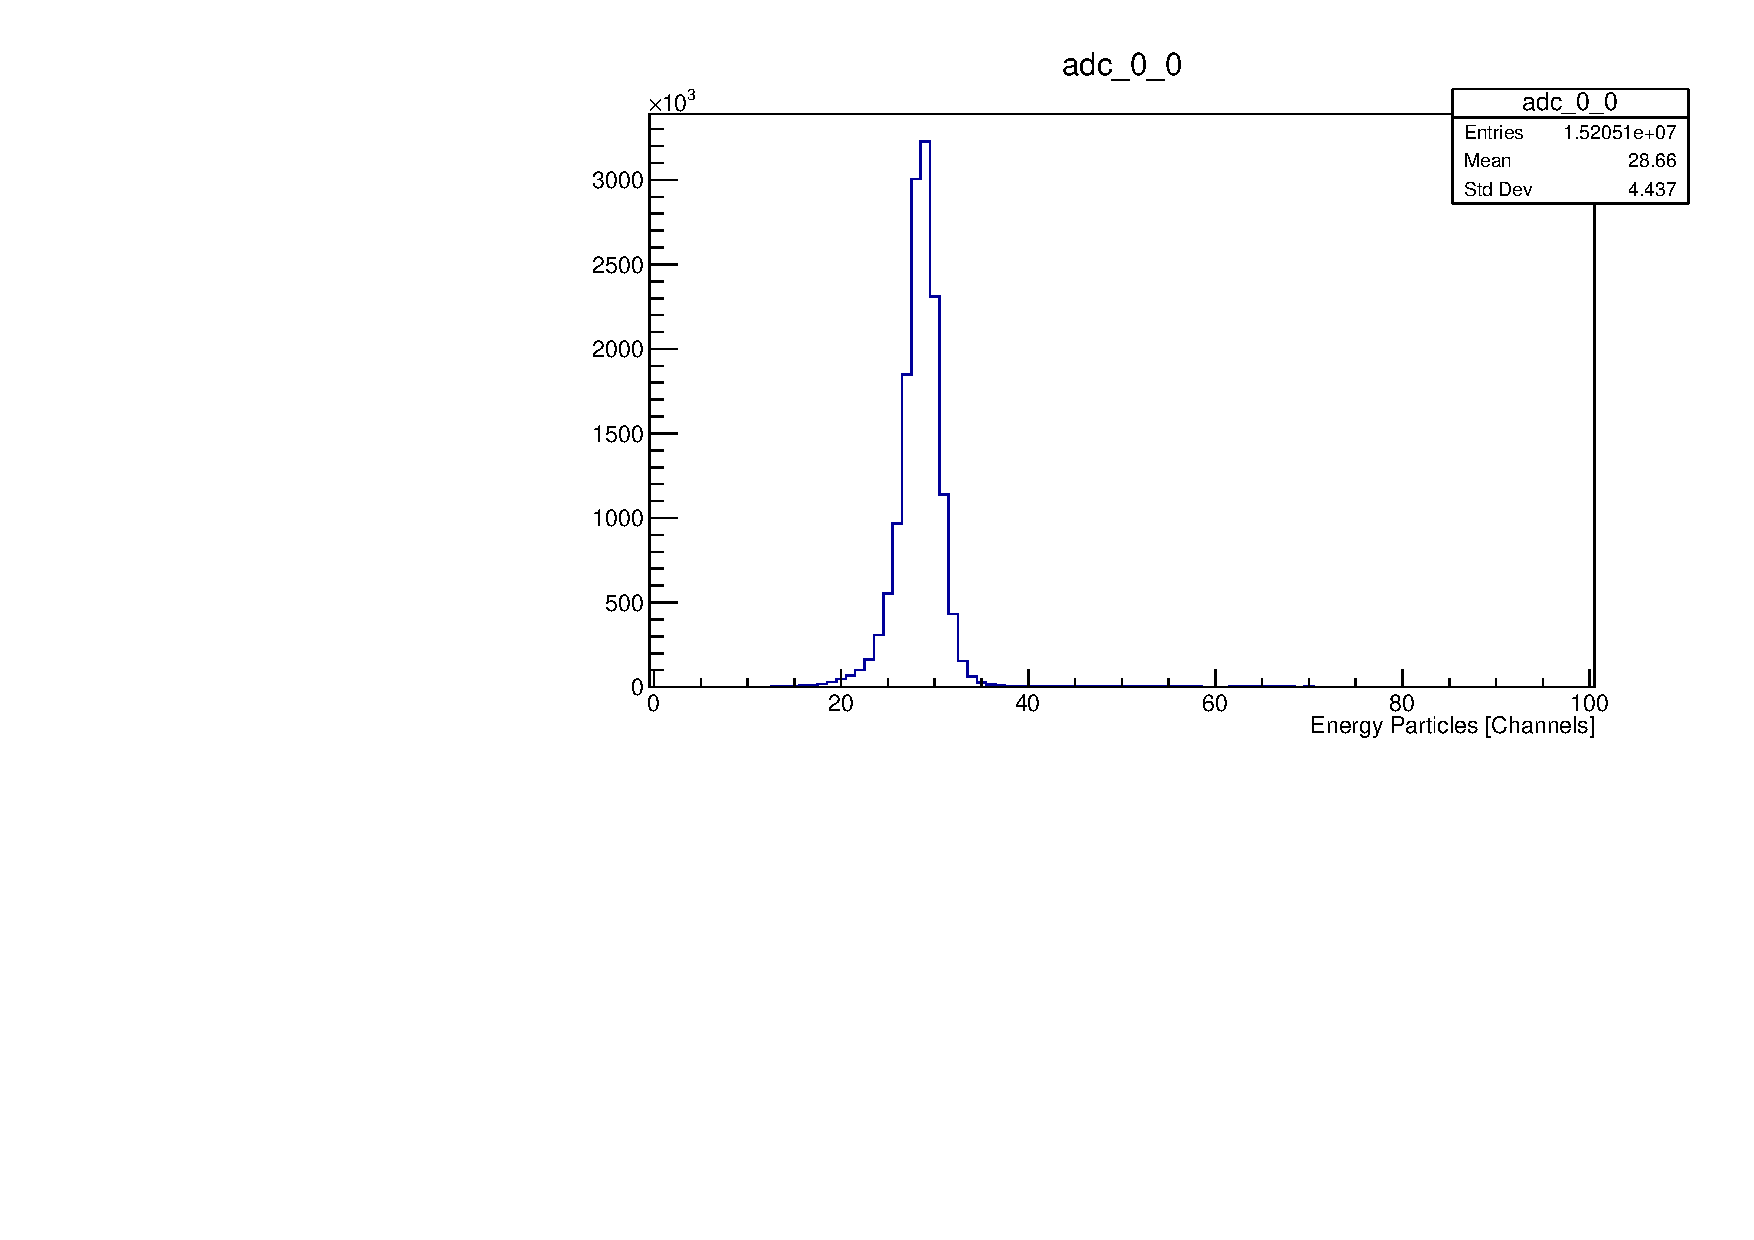
\includegraphics[width=\textwidth]{../Plots/plotting/Pedestal_Q1_f1.pdf}
	\caption{Pedestal Q1, f1.}
	\label{fig:Pedestal_f}
\end{figure}

\begin{figure}[ht]
	\centering
	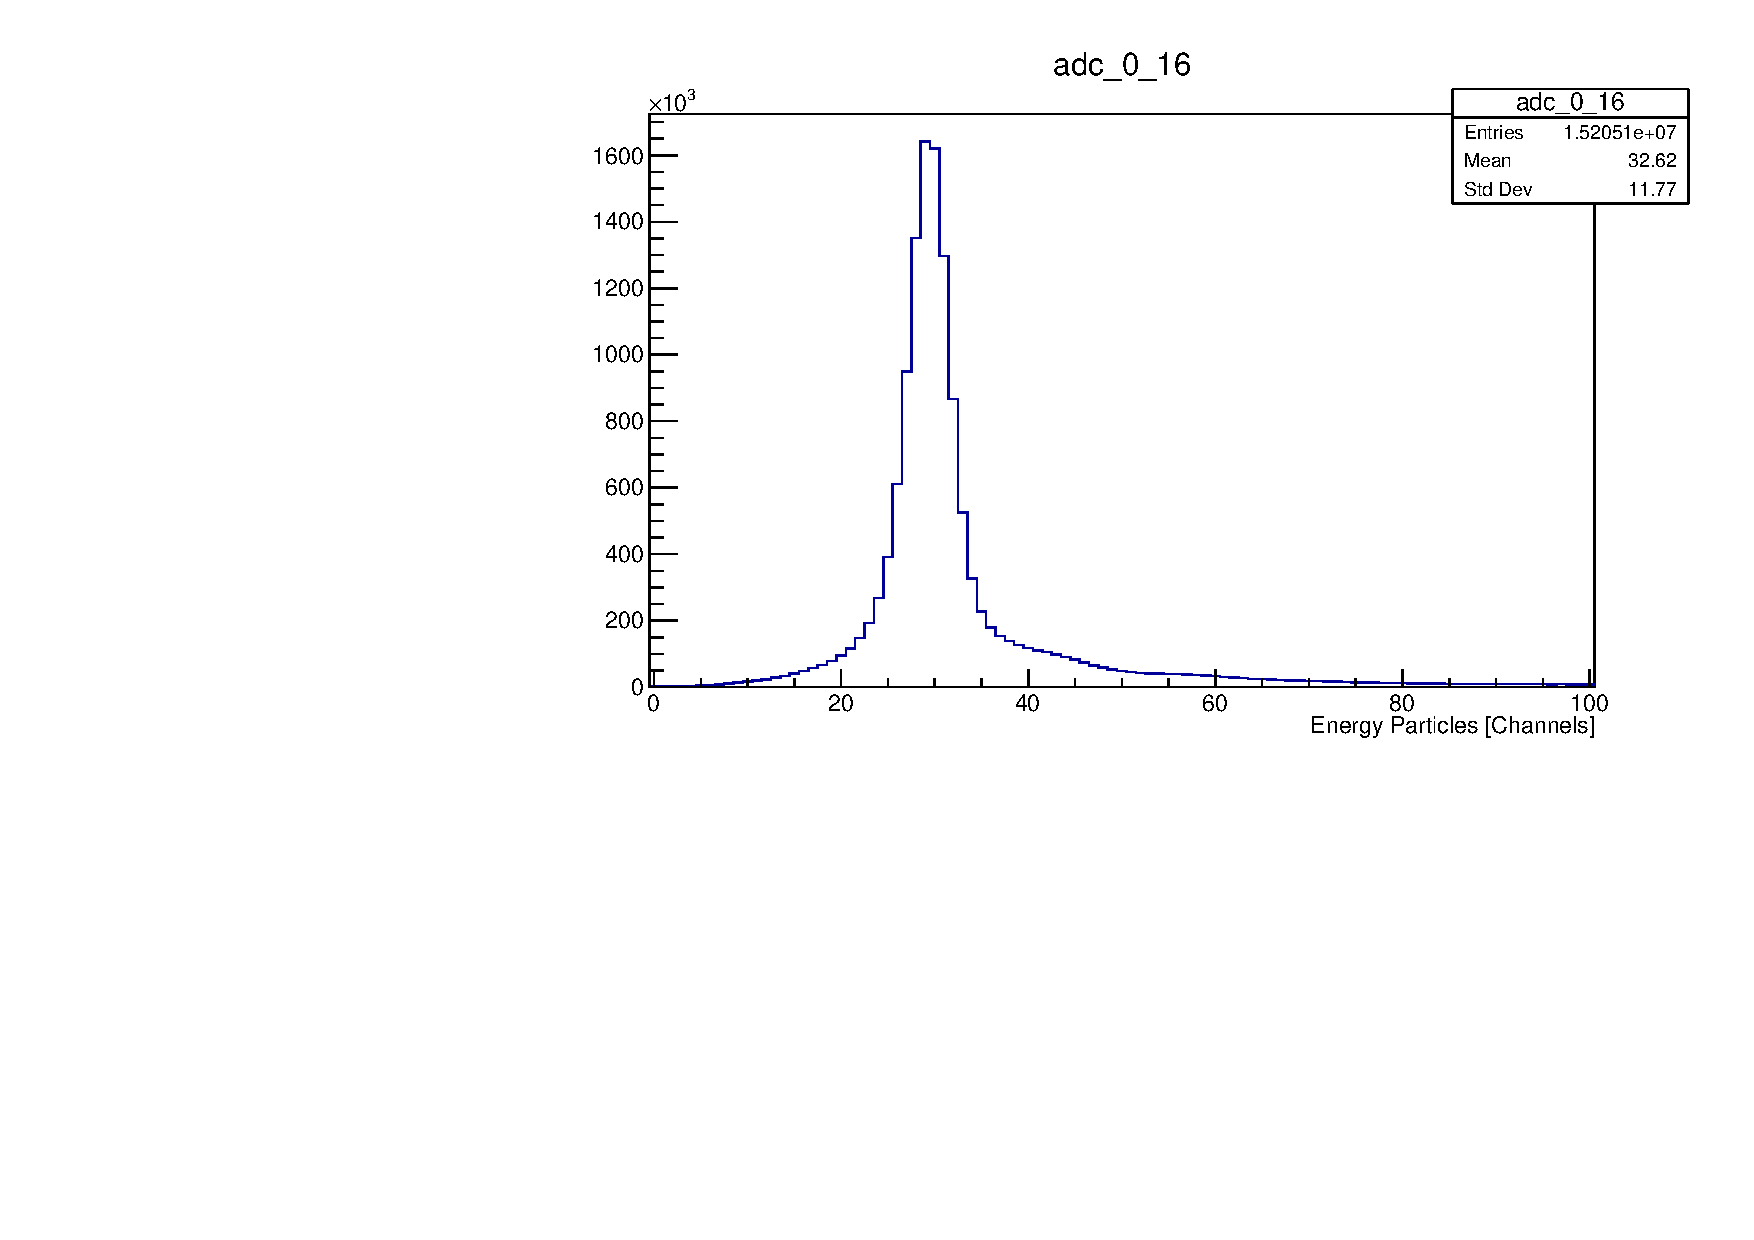
\includegraphics[width=\textwidth]{../Plots/plotting/Pedestal_Q1_b1.pdf}
	\caption{Pedestal Q1, b1.}
	\label{fig:Pedestal_b}
\end{figure}



\textbf{Threshold}

* Threshold (forskjellig i log/ikke-log skala)

Using a logarithmic y-axis, the threshold value will decrease very much. So don't use that. 

\textcolor{Magenta}{Tilbakemelding: \newline 
easier to set thresholds on lin. scale.
}

Threshold: The code has a default threshold of 100, but in some cases this is too much and some cases this is not enough. So for each adc channel, the threshold can be set. We don't want to include the "pedestal". Charge sharing.
Won't cut too much or too little..

\begin{figure}[ht]
	\centering
	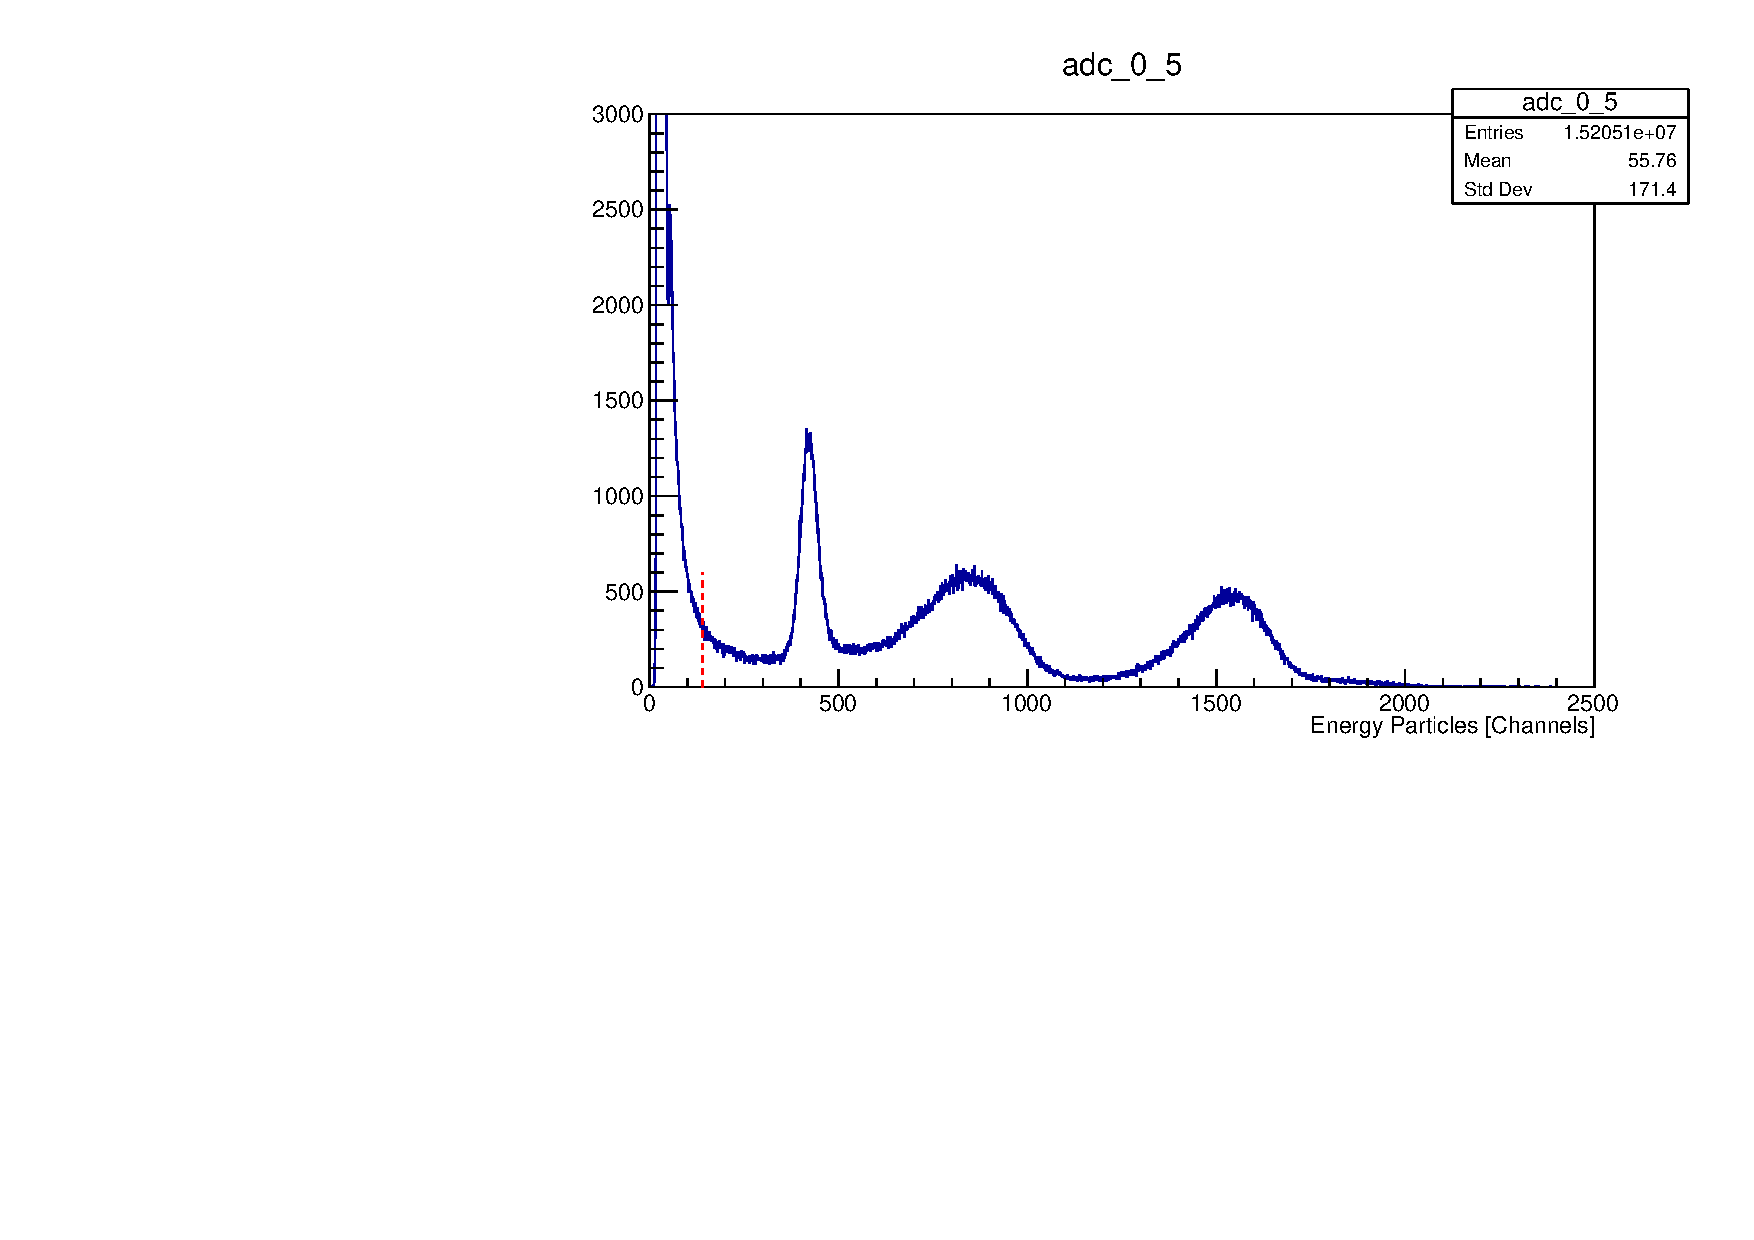
\includegraphics[width=\textwidth]{../Plots/plotting/Threshold_Q1_f6.pdf}
	\caption{Threshold Q1, f6.}
	\label{fig:Threshold_f}
\end{figure}


\begin{figure}[ht]
	\centering
	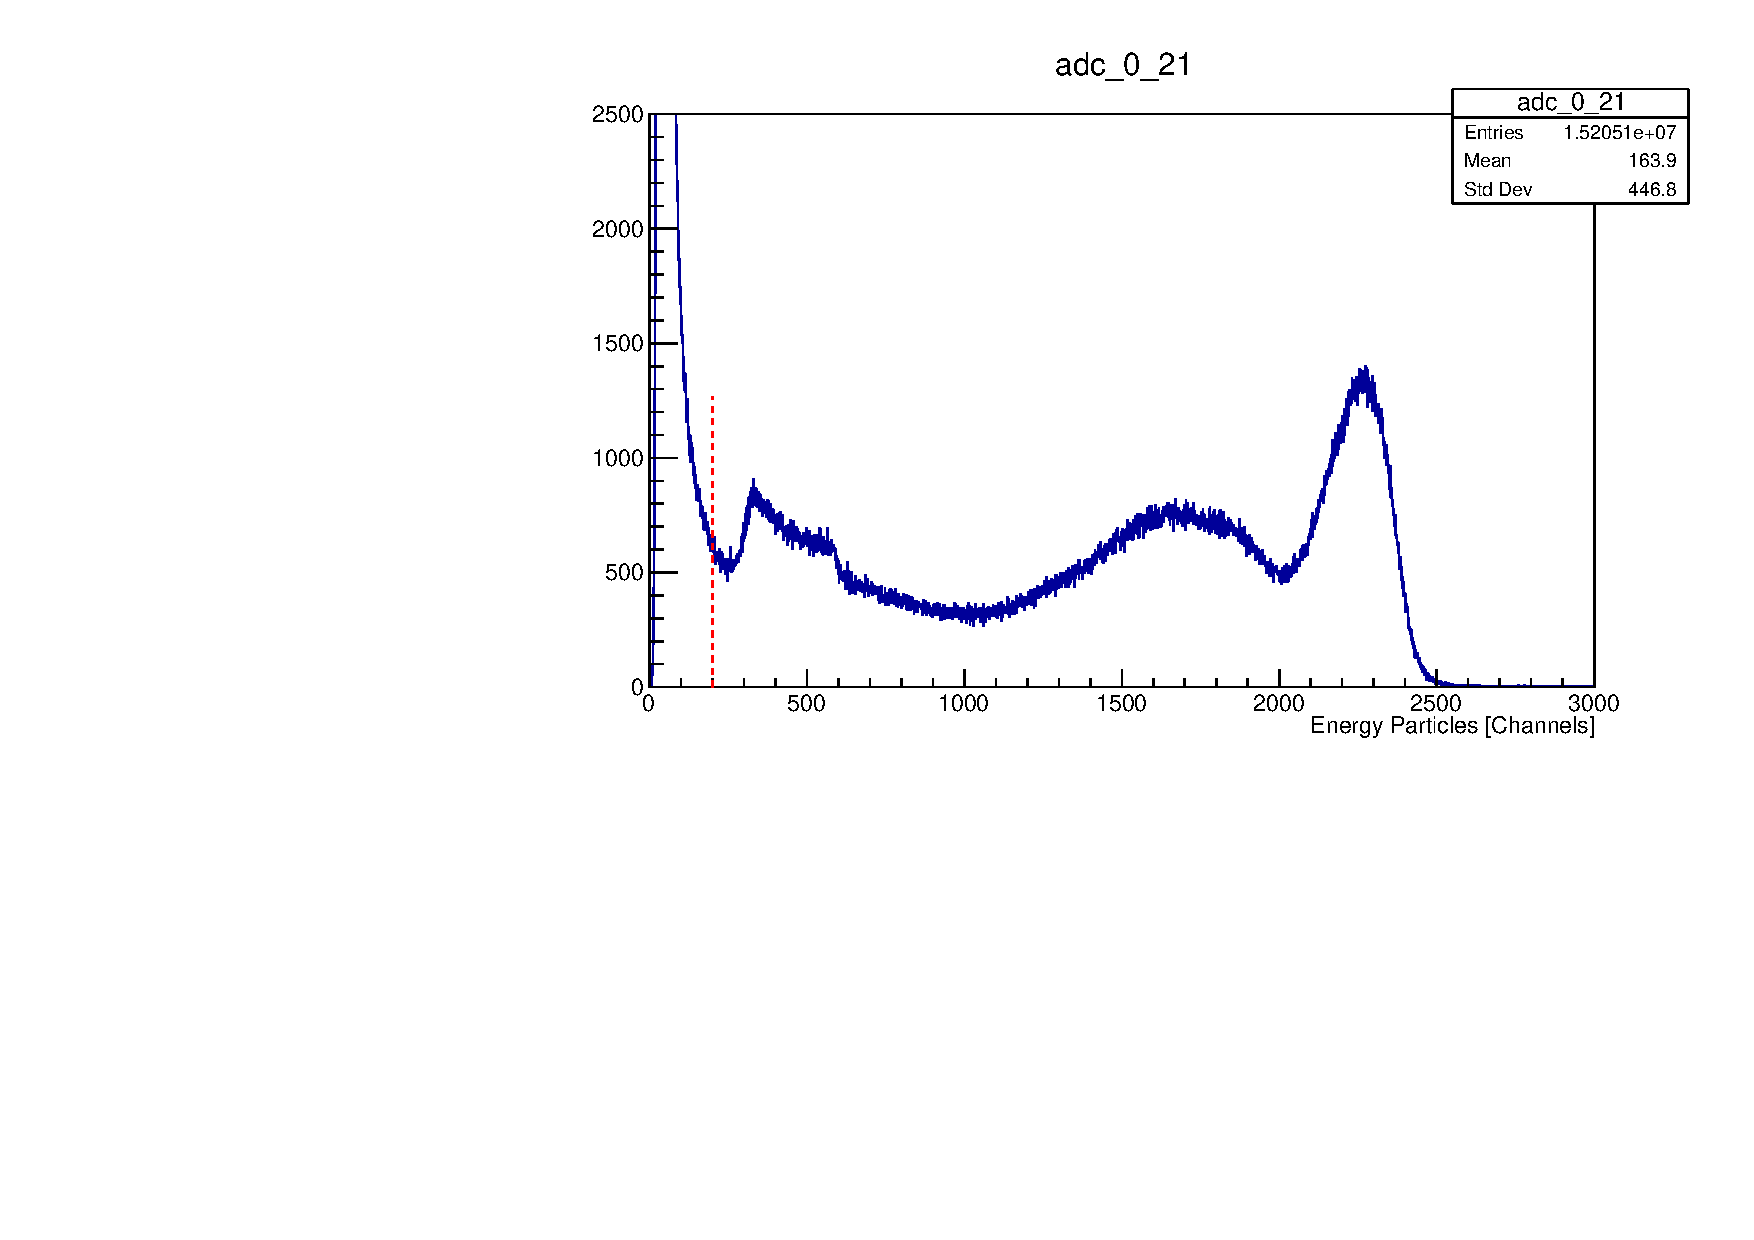
\includegraphics[width=\textwidth]{../Plots/plotting/Threshold_Q1_b6.pdf}
	\caption{Threshold Q1, b6.}
	\label{fig:Threshold_b}
\end{figure}


\textbf{CD debug:}

\begin{lstlisting}[language=sh]
$ cd /Users/trondwj/GitHub/MasterThesis/Scripts/plotting 
$ root
root [0] .L MultiPlot.cpp++
root [1] check_cd_debug("setup_Sm.txt")
\end{lstlisting}


\begin{figure}[ht]
	\centering
	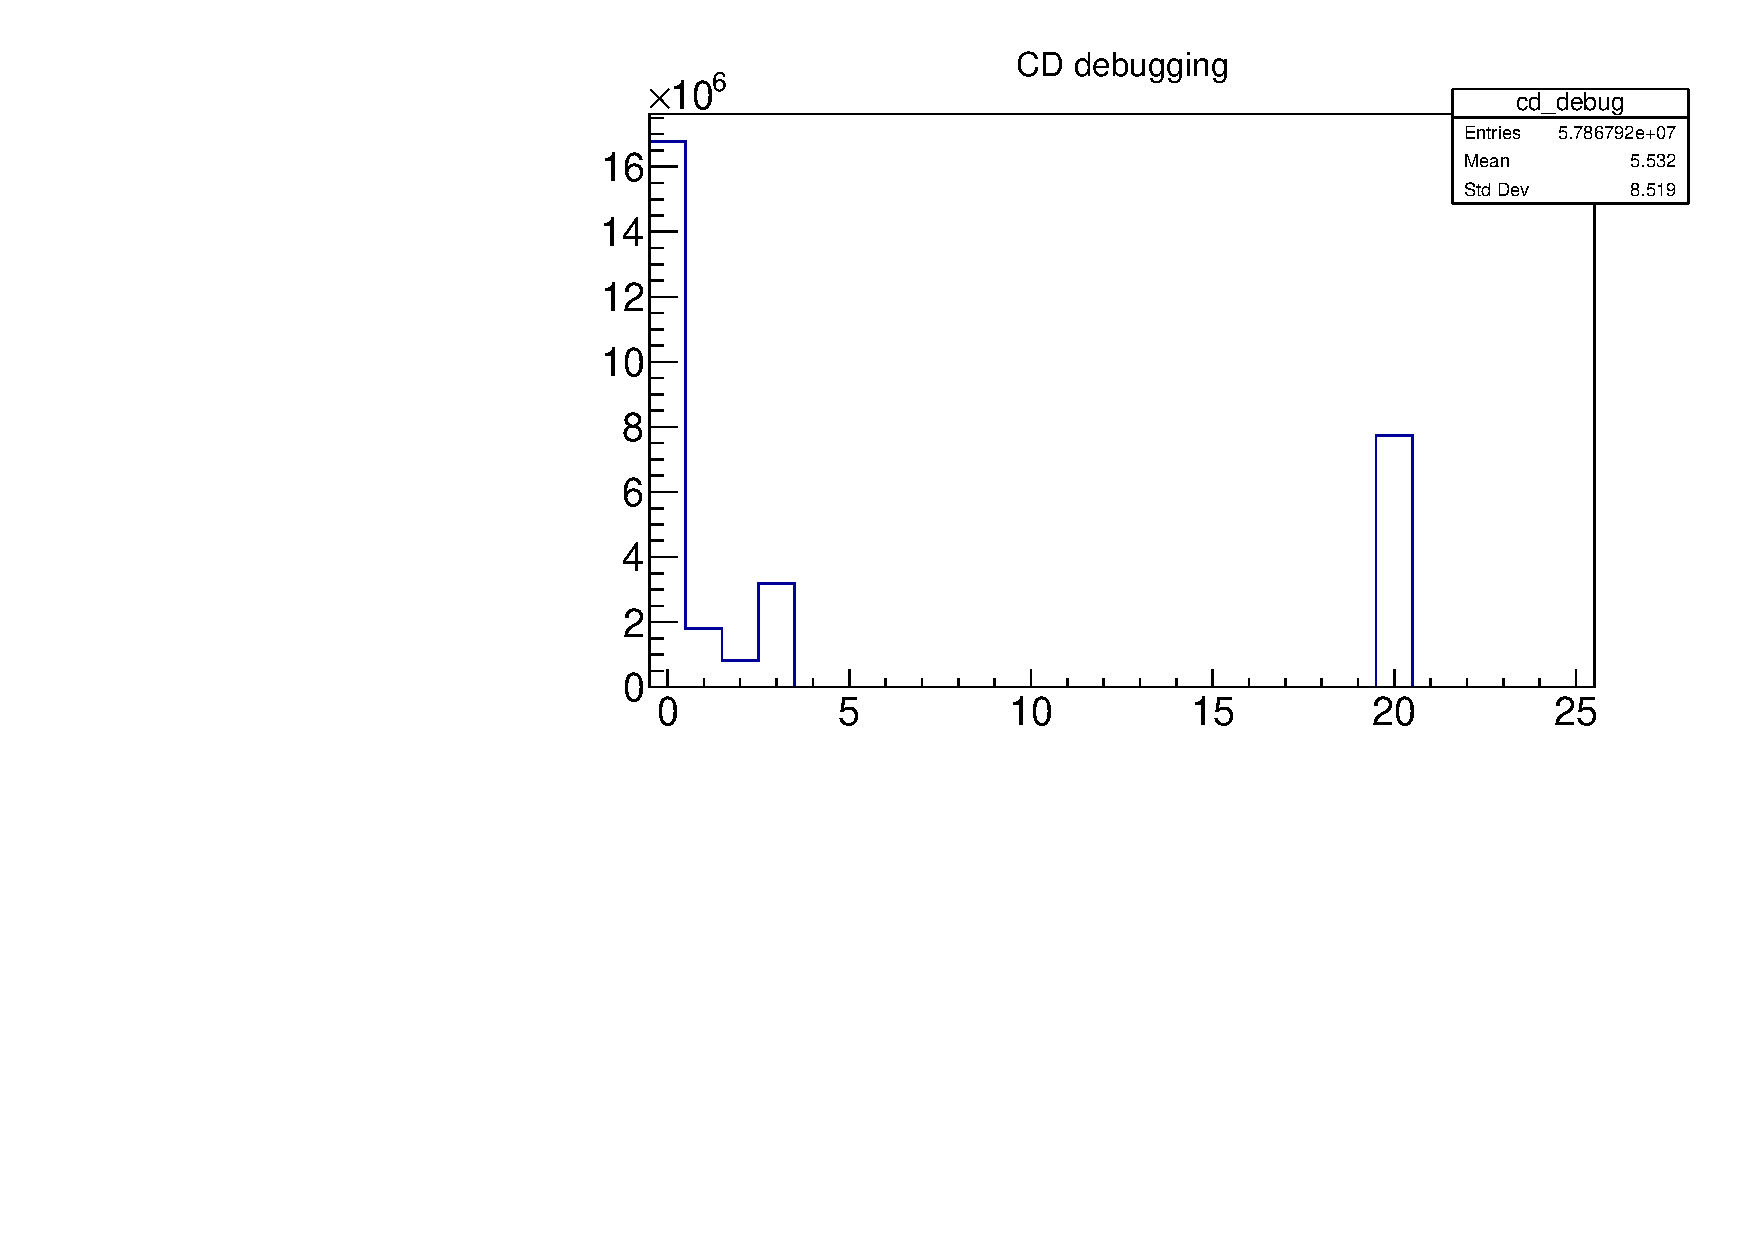
\includegraphics[width=\textwidth]{../Plots/plotting/cd_debug-user.pdf}
	\caption{CD debugging.}
	\label{fig:CD_debug}
\end{figure}


\subsection{Particle detector}


\subsubsection{User calibration}
ADC: Analog to digital converter (Mesytec)

TDC: Time to digital converter

DSSSD: Double-Sided Silicon Strip Detector $\implies$ CD

must remove the inner ring from data analysis because of damage

\begin{align*}
	\text{gain} = \frac{E_{\text{Sm}} - E_{\text{Pb}}}{Ch_{\text{Sm}} - Ch_{\text{Pb}}}
\end{align*}

\begin{align*}
	\text{offset} = E_{\text{Sm}} - \text{gain} \cdot Ch_{\text{Sm}}
\end{align*}
in keV.

\textcolor{red}{Hvis man har flere sentroider bruker man bare lineær regresjon. Gjelder spesielt for baksiden!}

\begin{figure}[ht]
	\centering
	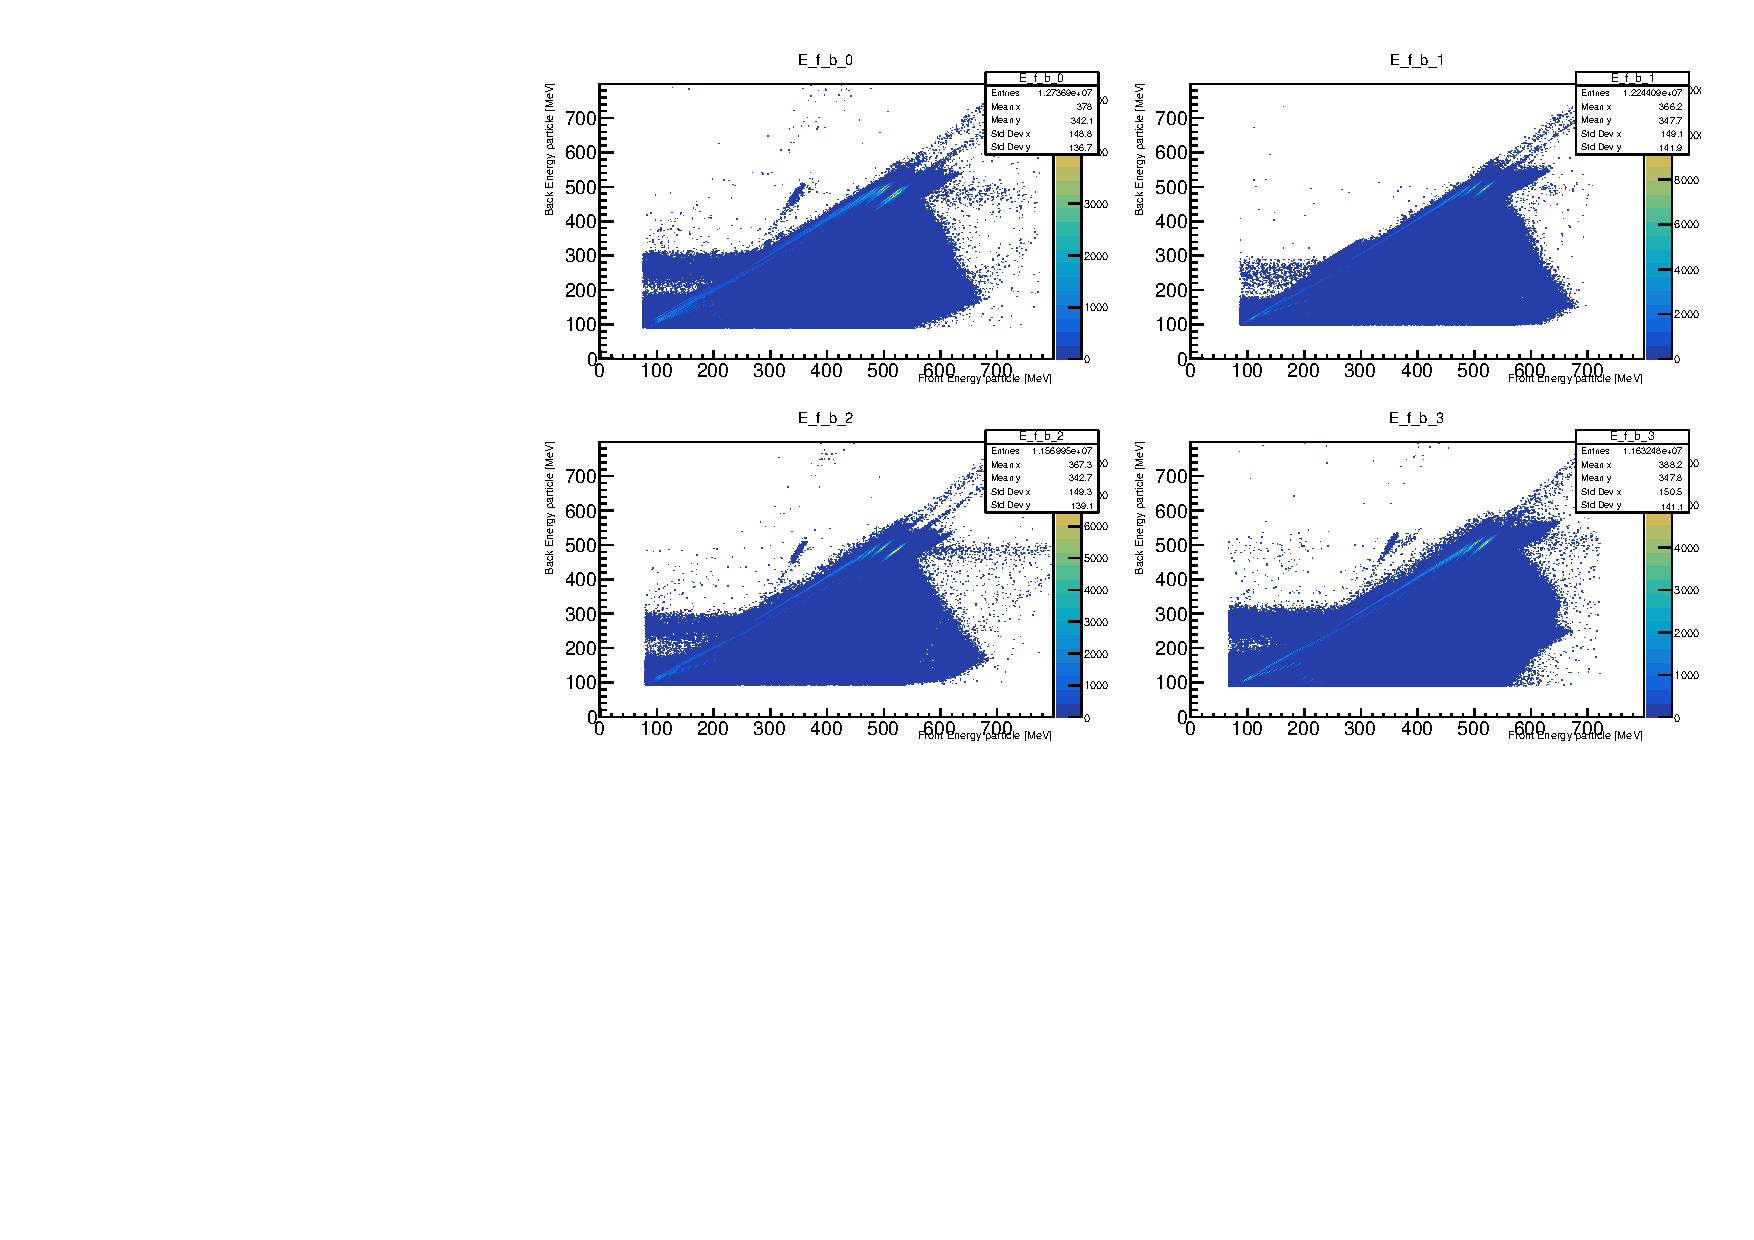
\includegraphics[width=\textwidth]{../Plots/plotting/E_f_b_Q1-4-user-new-cal.pdf}
	\caption{User calibration.}
	\label{fig:cal_user}
\end{figure}



\subsubsection{Online calibration}


\begin{figure}[ht]
	\centering
	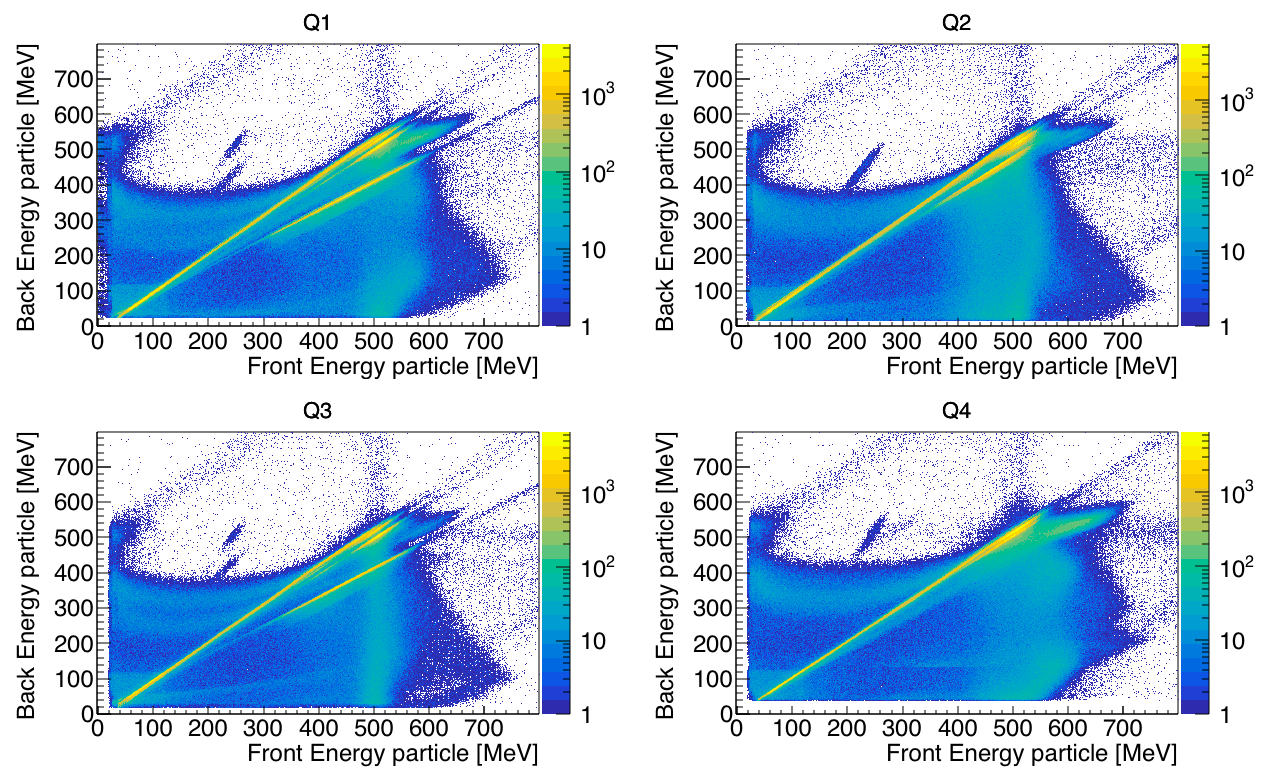
\includegraphics[width=\textwidth]{../Plots/plotting/E_f_b_Q1-4-online.pdf}
	\caption{Online calibration.}
	\label{fig:cal_online}
\end{figure}



\subsection{Gamma detectors}

DGF: Digital \ga~ finder

addback, singles, ...


\begin{table}[ht] 
	\centering 
	\caption{DGF}
	% Data for the DGF table
\begin{tabular}{cccc}
\hline
Cluster & Detector & Segment & TreeBuilder            \\
\hline
0       & 0        & 0       & E\_gam\_seg\_0\_0\_0   \\
\hline
\end{tabular}
	\label{tab:DGF}
\end{table}


\section{Doppler correction}





% ----------------------------------------------------------------------------------------------------------------------% ----------------------------------------------------------------------------------------------------------------------


\chapter{Experimental results}


Very pure beam (\textcolor{red}{did we have statistics of this?}) - resultat til avhandling. sjekk etter doppler-korrigering. Nd-contaminasjon? i så fall veldig lite, 1-2 prosent?

\textcolor{Magenta}{Tilbakemelding: \newline
we would have to look at the \ga-spectra to identify any contaminants. There may be a little bit of Nd-140 in the beam, but if so, it is very little (judging from on-line spectra).}


% ----------------------------------------------------------------------------------------------------------------------% ----------------------------------------------------------------------------------------------------------------------


\chapter{Discussion}

Level scheme (from Klintefjord?)\newline

\textcolor{Magenta}{Tilbakemelding: \newline
at some point you should show the level scheme. \newline
$\bullet$ motivation: to explain what is known, and which transition probabilities you want to measure.  \newline
Perhaps also to explain what theory predicts. \newline
$\bullet$ discussion: if you get \ga-spectrum for \Sm\ $\rightarrow$ to explain what you see.}


\begin{figure}
	\centering
	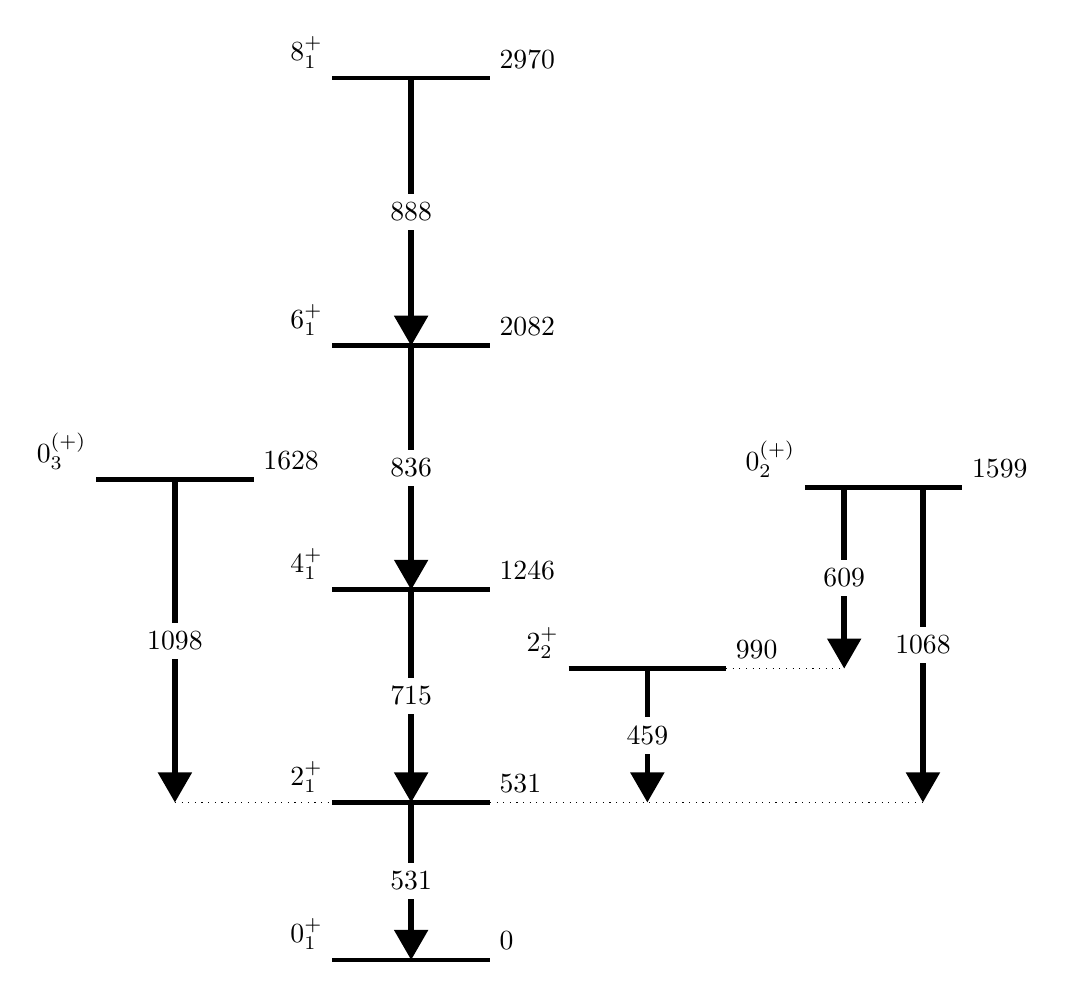
\begin{tikzpicture}[
    level/.style = { ultra thick, black },
    connect/.style = { dotted, black },
    notice/.style = { draw, rectangle callout, callout relative pointer={#1} },
    label/.style = { text width=2cm }
    ]
    %%% Picture made by normalizing energy to the 2+ state (531) and choosing it to be 
    %%% 2 units of y in height.

    %%%
    %%% Ground state band
    %%%
    % Levels, states, energy
    \foreach \level / \state / \energy in {0/0_1^+/0, 2/2_1^+/531, 4.7/4_1^+/1246, 7.8/6_1^+/2082, 11.2/8_1^+/2970}
      { 
        \draw[level] (0,\level) -- (2,\level);
        \node at (0,\level) [anchor=south east] {$\state$};
        \node at (2,\level) [anchor=south west] {$\energy$};
      }
    % Gamma transitions
    \foreach \endlevel / \startlevel / \gamma in {0/2/531, 2/4.7/715, 4.7/7.8/836, 7.8/11.2/888}
      { 
        \draw[line width=2pt, ->, >=triangle 60] (1,\startlevel) -- node[fill=white] {\gamma} (1,\endlevel);
      }
    % Dotted lines
    \draw[connect] (-2,2) -- (0,2) (2,2) -- (7.5,2);
    %\draw[connect] (-2,11.2) -- (0,11.2) (2,11.2) -- (4,11.2);
    
    %%%
    %%% Left band
    %%%
    % Lower left band
    \coordinate (levelleft)  at (-3,6.1);
    \coordinate (levelright) at (-1,6.1);
    \draw[level] (levelleft) -- (levelright);
    \node at (levelleft)  [anchor=south east] {$0_3^{(+)}$};
    \node at (levelright) [anchor=south west] {1628};
    \draw[line width=2pt, ->, >=triangle 60] (-2,6.1) -- node[fill=white] {1098} (-2,2);
    %% Higher left band
    %\foreach \level / \state / \energy in {12.1/10^+/3211, 13.8/12^+/3653, 16.6/14^+/4404, 20.3/16^+/5398}
    %  { 
    %    \draw[level] (-3,\level) -- (-1,\level);
    %    \node at (-3,\level) [anchor=south east] {$\state$};
    %    \node at (-1,\level) [anchor=south west] {$\energy$};
    %  }
    %% Gamma transitions
    %\foreach \endlevel / \startlevel / \gamma in {12.1/13.8/442, 13.8/16.6/751, 16.6/20.3/994}
    %  { 
    %    \draw[line width=2pt, ->, >=triangle 60] (-2,\startlevel) -- node[fill=white] {\gamma} (-2,\endlevel);
    %  }
    %% First gamma transition
    %\draw[line width=2pt, ->, >=triangle 60] (-2,12.1) -- node[left=3pt] {241} (-2,11.2);

    %%%
    %%% 1st right band
    %%%
    % Lower 1st right band
    \coordinate (levelleft)  at (3,3.7);
    \coordinate (levelright) at (5,3.7);
    \draw[level] (levelleft) -- (levelright);
    \node at (levelleft)  [anchor=south east] {$2_2^+$};
    \node at (levelright) [anchor=south west] {990};
    \draw[line width=2pt, ->, >=triangle 60] (4,3.7) -- node[fill=white] {459} (4,2);
    % Dotted lines
    \draw[connect] (levelright) -- (6.5,3.7);
    %% Higher 1st right band; levels, states, energy
    %\foreach \level / \state / \energy in {11.9/10^+/3172, 14.3/12^+/3791, 18.5/14^+/4914}
    %  { 
    %    \draw[level] (3,\level) -- (5,\level);
    %    \node at (3,\level) [anchor=south east] {$\state$};
    %    \node at (5,\level) [anchor=south west] {$\energy$};
    %  }
    %% Gamma transitions
    %\foreach \endlevel / \startlevel / \gamma in {11.9/14.3/619, 14.3/18.5/1123}
    %  { 
    %    \draw[line width=2pt, ->, >=triangle 60] (4,\startlevel) -- node[fill=white] {\gamma} (4,\endlevel);
    %  }
    %% First gamma transition
    %\draw[line width=2pt, ->, >=triangle 60] (4,11.9) -- node[right=4pt] {202} (4,11.2);

    %%%
    %%% 2nd right band
    %%%
    \coordinate (levelleft)  at (6,6);
    \coordinate (levelright) at (8,6);
    \draw[level] (levelleft) -- (levelright);
    \node at (levelleft)  [anchor=south east] {$0_2^{(+)}$};
    \node at (levelright) [anchor=south west] {1599};
    \draw[line width=2pt, ->, >=triangle 60] (7.5,6) -- node[fill=white] {1068} (7.5,2);
    \draw[line width=2pt, ->, >=triangle 60] (6.5,6) -- node[fill=white] {609} (6.5,3.7);    
\end{tikzpicture}
	\caption{Level scheme for \Sm. Adapted from Klintefjord.}
	\label{fig:levels}
\end{figure}




% ----------------------------------------------------------------------------------------------------------------------% ----------------------------------------------------------------------------------------------------------------------

\chapter{Summary and outlook}

Future work: Better calibration of particle detectors (online not perfect). Take into account the shape of the peaks $\implies$ calibrate the particle detectors manually.. Takes a lot of time! But maybe less than trying to fit all in a script? Had I just known...


\textcolor{red}{Fra oppgaveteksten:} \newline
determine Coulomb excitation yields. These yields will then, in a second step, be compared to theoretical calculations and transition probabilities and quadrupole moments will be extracted using chi-square minimization procedures.


GOSIA and GOSIA2 analysis?

\url{https://www.pas.rochester.edu/~cline/Gosia/Gosia_Manual_20110609.pdf}

% ----------------------------------------------------------------------------------------------------------------------% ----------------------------------------------------------------------------------------------------------------------




% ----------------------------------------------------------------------------------------------------------------------% ----------------------------------------------------------------------------------------------------------------------

\begin{appendices}

\chapter{Symbol list}

\begin{table}[h]
  \centering
  \caption{Table of symbols with explanations.}
    \begin{tabular}{ll}
        \hline
        T$_{1/2}$ & Half-life \\
        \hline
    \end{tabular}
    \label{tab:symbols}
\end{table}


\chapter{Acronyms and abbreviations}

\begin{table}[ht] 
	\centering 
	\caption{Table of acronyms and abbreviations.}
	% Data for the Acronyms and abbreviations table
\begin{tabular}{ll}
    \hline
    ADC         &  Analog to Digital Converter                                \\
    bash        &  Bourne-Again SHell                                         \\
    CERN        &  European Council for Nuclear Research                      \\ 
                &  (in French: Conseil Européen pour la Recherche Nucléaire)  \\
    CD          &  Compact Disc                                               \\
    COULEX      &  COULomb EXcitation                                         \\
    DAQ         &  Data AcQuisition                                           \\
    DGF         &  Digital Gamma Finder                                       \\
    DSSSD       &  Double Sided Silicon Strip Detector (also known as CD)     \\
    GPS         &  General Purpose Separator                                  \\
    HRS         &  High Resolution Separator                                  \\
    HIE-ISOLDE  &  High Intensity and Energy upgrade at ISOLDE                \\
    HPGe        &  High Purity Germanium                                      \\
    ISOL        &  Isotope Separator On Line                                  \\
    ISOLDE      &  ISOL DEvice                                                \\
    LINAC       &  LINear ACcelerator                                         \\
    MBS         &  Multi Branch System                                        \\
    MED         &  MBS Event Data (also known as Miniball Event Data)         \\
    MAR\belowbaseline[-2pt]{a}B\stackinset{l}{3pt}{b}{-3pt}{O}{O}\,U     
                &  MBS And ROOT Based Online/Offline Utility                  \\
    PSB         &  Proton Synchrotron Booster                                 \\
    REX         &  Radioactive beam EXperiment                                \\
    EBIS        &  Electron Beam Ion Source                                   \\
    REXEBIS     &  Radioactive beam EXperiment Electron Beam Ion Source       \\
    REXTRAP     &  Radioactive beam EXperiment TRAP                           \\
    REX-ISOLDE  &  Radioactive beam EXperiment at ISOLDE                      \\
    RIB         &  Radioactive Ion Beam                                       \\
    RILIS       &  Resonance Ionization Laser Ion Source                      \\
    SRIM        &  Stopping and Range of Ions in Matter                       \\
    TDC         &  Time to Digital Converter                                  \\
    \hline
\end{tabular}
\label{tab:acro}

\end{table}


\chapter{Two-particle collision}
\section{Laboratory (LAB) frame of reference}\label{sec:LAB}
The angles of the two-particle collision in the laboratory frame from \autoref{fig:LAB} is calculated in this section. A general approach is used to make it easier to hold track of the parameters. From the figure we can express the velocities as
\begin{align}\label{eq:2p-LAB-collision}
\begin{split}
	 \boldsymbol{u} &= \boldsymbol{u}_1 = u \boldsymbol{\hat{x}}  \\
	 \boldsymbol{u}_2 &= 0  \\
	 \boldsymbol{v}_b &= \boldsymbol{v}_1 = v_1 (\cos \theta \boldsymbol{\hat{x}} + \sin \theta \boldsymbol{\hat{y}})  \\
	\boldsymbol{v}_t &= \boldsymbol{v}_2 = v_2 (\cos \varphi \boldsymbol{\hat{x}} - \sin \varphi \boldsymbol{\hat{y}})
\end{split}
\end{align}
where $\boldsymbol{u}_1$ and $\boldsymbol{v}_1$ is the initial and final velocity of the projectile $m_b = m_1$ respectively, and $\boldsymbol{u}_2$ and $\boldsymbol{v}_2$ is the initial and final velocity of the target $m_t = m_2$ respectively. The angles $\theta_b = \theta$ and $\theta_t = \varphi$ are the projectile and target angle respectively. We also introduce a ratio of the projectile mass to the target mass, $\alpha = m_1/m_2$.

Conservation of momentum gives
\begin{align*}%\label{eq:comom}
	m_1 \boldsymbol{u}_1 &= m_1 \boldsymbol{v}_1 + m_2 \boldsymbol{v}_2
\end{align*}
which in x-direction can be expressed as
\begin{align}\label{eq:comx}
	m_1 u &= m_1 v_1 \cos \theta + m_2 v_2 \cos \varphi  \nonumber\\
	m_1 (u - v_1 \cos \theta) &= m_2 v_2 \cos \varphi  \nonumber\\
	\frac{m_1}{m_2} (u - v_1 \cos \theta) &= v_2 \cos \varphi  \nonumber\\
	\alpha (u - v_1 \cos \theta) &= v_2 \cos \varphi
\end{align}
and in y-direction can be expressed as
\begin{align}\label{eq:comy}
	0 &= m_1 v_1 \sin \theta - m_2 v_2 \sin \varphi \nonumber\\
	m_1 v_1 \sin \theta &= m_2 v_2 \sin \varphi \nonumber\\
	\frac{m_1}{m_2} v_1 \sin \theta &= v_2 \sin \varphi \nonumber\\
	\alpha v_1 \sin \theta &= v_2 \sin \varphi
\end{align}

Conservation of energy gives
\begin{align}\label{eq:coe}
	\tfrac{1}{2} m_1 \boldsymbol{u}_1^2 &= \tfrac{1}{2} m_1 \boldsymbol{v}_1^2 + \tfrac{1}{2} m_2 \boldsymbol{v}_2^2 \nonumber\\
	\tfrac{1}{2} m_1 (u^2 - v_1^2) &= \tfrac{1}{2} m_2 v_2^2 \nonumber\\
	\frac{m_1}{m_2} (u^2 - v_1^2) &= v_2^2 \nonumber\\
	\alpha (u^2 - v_1^2) &= v_2^2
\end{align}

We now have three equations (\autoref{eq:comx} - \autoref{eq:coe}) with four unknown quantities ($v_1, \theta, v_2, \varphi$). Using the target angle $\varphi$ as an independent variable, we can find expressions for the other three variables. 

Squaring \autoref{eq:comx} 
\begin{align*}%\label{eq:c}
	\alpha^2 (u - v_1 \cos \theta)^2 &= v_2^2 \cos^2 \varphi  \\
	\alpha^2 (u^2 - 2uv_1 \cos \theta + v_1^2 \cos^2 \theta) &= v_2^2 \cos^2 \varphi
\end{align*}
and \autoref{eq:comy}
\begin{align*}%\label{eq:c}
	\alpha^2 v_1^2 \sin^2 \theta &= v_2^2 \sin^2 \varphi
\end{align*}
and adding them together gives
\begin{align}\label{eq:av}
	\alpha^2 (u^2 - 2uv_1 \cos \theta + v_1^2 \cos^2 \theta + v_1^2 \sin^2 \theta) &= v_2^2 (\cos^2 \varphi + \sin^2 \varphi)  \nonumber\\
	\alpha^2 (u^2 - 2uv_1 \cos \theta + v_1^2) &= v_2^2  \nonumber\\
	\alpha^2 u^2 - 2\alpha^2 uv_1 \cos \theta + \alpha^2 v_1^2 &= v_2^2  \nonumber\\
	\alpha^2 v_1^2 &= -\alpha^2 u^2 + 2\alpha^2 uv_1 \cos \theta + v_2^2  \nonumber\\
	\alpha^2 v_1^2 &= -\alpha^2 u^2 + 2\alpha u (\alpha v_1 \cos \theta) + v_2^2
\end{align}
From \autoref{eq:comx} we have
\begin{align}\label{eq:comx2}
	\alpha (u - v_1 \cos \theta) &= v_2 \cos \varphi  \nonumber\\
	\alpha u - \alpha v_1 \cos \theta &= v_2 \cos \varphi  \nonumber\\
	\alpha v_1 \cos \theta &= \alpha u - v_2 \cos \varphi
\end{align}
Substituting for \autoref{eq:comx2} into \autoref{eq:av} we get
\begin{align}\label{eq:comsq}
	\alpha^2 v_1^2 &= -\alpha^2 u^2 + 2\alpha u (\alpha u - v_2 \cos \varphi ) + v_2^2  \nonumber\\
	\alpha^2 v_1^2 &= -\alpha^2 u^2 + 2\alpha^2 u^2 - 2\alpha u v_2 \cos \varphi + v_2^2  \nonumber\\
	\alpha^2 v_1^2 &= \alpha^2 u^2 - 2\alpha u v_2 \cos \varphi + v_2^2
\end{align}
Using \autoref{eq:coe} we get
\begin{align}\label{eq:coesub}
    \left( \frac{\alpha}{\alpha} \right) \alpha (u^2 - v_1^2) &= v_2^2  \nonumber\\
    \alpha^2 (u^2 - v_1^2) &= \alpha v_2^2  \nonumber\\
	\alpha^2 u^2 - \alpha^2 v_1^2 &= \alpha v_2^2  \nonumber\\
	\alpha^2 v_1^2 &= \alpha^2 u^2 - \alpha v_2^2
\end{align}
Combining \autoref{eq:comsq} and \autoref{eq:coesub} gives
\begin{align}\label{eq:comcoe}
    \alpha^2 u^2 - 2\alpha u v_2 \cos \varphi + v_2^2 &= \alpha^2 u^2 - \alpha v_2^2  \nonumber\\
    v_2^2 + \alpha v_2^2 &= 2\alpha u v_2 \cos \varphi  \nonumber\\
    v_2^2 (1 + \alpha) &= 2\alpha u v_2 \cos \varphi  \nonumber\\
    v_2 &= 2 \left( \frac{\alpha}{1 + \alpha} \right) u \cos \varphi 
\end{align}
Substituting \autoref{eq:comcoe} into \autoref{eq:coesub} we get
\begin{align}\label{eq:coesubsub}
    \alpha^2 v_1^2 &= \alpha^2 u^2 - \alpha \left( 2 \left( \frac{\alpha}{1 + \alpha} \right) u \cos \varphi  \right)^2  \nonumber\\
    v_1^2 &= u^2 - \frac{1}{\alpha} \left( 4 \left( \frac{\alpha^2}{(1 + \alpha)^2} \right) u^2 \cos^2 \varphi  \right)  \nonumber\\
    v_1^2 &= u^2 \left(1 - 4 \left( \frac{\alpha}{(1 + \alpha)^2} \right) \cos^2 \varphi  \right)  \nonumber\\
    v_1 &= u \sqrt{1 - 4 \frac{\alpha}{M} \cos^2 \varphi}
\end{align}
where $\alpha/M = \alpha/(1 + \alpha)^2$. The ratio of \autoref{eq:comy} and \autoref{eq:comx2} gives
\begin{align}\label{eq:comxy}
	\frac{\alpha v_1 \sin \theta}{\alpha v_1 \cos \theta} &= \frac{v_2 \sin \varphi}{\alpha u - v_2 \cos \varphi}  \nonumber\\
	\tan \theta &= \frac{v_2 \sin \varphi}{\alpha u - v_2 \cos \varphi}
\end{align}
Inserting \autoref{eq:comcoe} into \autoref{eq:comxy} gives
\begin{align}\label{eq:tanBgen}
	\tan \theta &= \frac{\left( 2 \left( \frac{\alpha}{1 + \alpha} \right) u \cos \varphi  \right) \sin \varphi}{\alpha u - \left( 2 \left( \frac{\alpha}{1 + \alpha} \right) u \cos \varphi  \right) \cos \varphi}  \nonumber\\
	\tan \theta &= \frac{\alpha u \left( \frac{1}{1 + \alpha} \right) 2 \sin \varphi \cos \varphi}{\alpha u \left(1 - 2 \left( \frac{1}{1 + \alpha} \right) \cos^2 \varphi \right)}  \nonumber\\
	\tan \theta &= \frac{\sin 2\varphi}{(1 + \alpha)\left(1 - 2 \left( \frac{1}{1 + \alpha} \right) \cos^2 \varphi \right)}  \nonumber\\
	\tan \theta &= \frac{\sin 2\varphi}{1 + \alpha - 2 \cos^2 \varphi}  \nonumber\\
	\tan \theta &= \frac{\sin 2\varphi}{\alpha - (2 \cos^2 \varphi - 1)}  \nonumber\\
	\tan \theta &= \frac{\sin 2\varphi}{\alpha - \cos 2\varphi}  \nonumber\\
	\theta &= \arctan \left( \frac{\sin 2\varphi}{\alpha - \cos 2\varphi} \right)
\end{align}
Substituting back the variable names from \autoref{fig:LAB} into \autoref{eq:tanBgen} gives
\begin{align}\label{eq:tanB}
	\theta_b &= \arctan \left( \frac{\sin 2\theta_t}{\alpha - \cos 2\theta_t} \right)
\end{align}


\section{Center of mass (CM) frame of reference}
Using the same approach as \autoref{sec:LAB}. From figure \autoref{fig:CM} we can express the velocities as
\begin{align}\label{eq:2p-CM-collision}
\begin{split}
	 \boldsymbol{u}_1^{'} &= u_1^{'} \boldsymbol{\hat{x}} \\
	 \boldsymbol{u}_2^{'} &= u_2^{'} \boldsymbol{\hat{x}} \\
	 \boldsymbol{v}_b^{'} &= \boldsymbol{v}_1^{'} = v_1^{'} (\cos \theta^{'} \boldsymbol{\hat{x}} + \sin \theta^{'} \boldsymbol{\hat{y}}) \\
	\boldsymbol{v}_t^{'} &= \boldsymbol{v}_2^{'} = v_2^{'} (-\cos \theta^{'} \boldsymbol{\hat{x}} - \sin \theta^{'} \boldsymbol{\hat{y}}) = -v_2^{'} (\cos \theta^{'} \boldsymbol{\hat{x}} + \sin \theta^{'} \boldsymbol{\hat{y}})
\end{split}
\end{align}
where $\boldsymbol{u}_1^{'}$ and $\boldsymbol{v}_1^{'}$ is the initial and final velocity of the projectile $m_b = m_1$ respectively, and $\boldsymbol{u}_2^{'}$ and $\boldsymbol{v}_2^{'}$ is the initial and final velocity of the target $m_t = m_2$ respectively. The angle $\theta_b^{'} = \theta^{'}$ is the projectile angle. 

In the center of mass (CM) frame of reference, the position of the center of mass is given by
\begin{align}\label{eq:CMpos}
	\boldsymbol{R} &= \frac{m_1 \boldsymbol{r}_1 + m_2 \boldsymbol{r}_2}{m_1 + m_2}
\end{align}
and the velocity is
\begin{align}\label{eq:Vcm}
	\boldsymbol{V} &= \frac{d\boldsymbol{R}}{dt}
	= \frac{d}{dt} \left( \frac{m_1 \boldsymbol{r}_1 + m_2 \boldsymbol{r}_2}{m_1 + m_2} \right)
	= \frac{m_1 \boldsymbol{u}_1^{'} + m_2 \boldsymbol{u}_2^{'}}{m_1 + m_2}
\end{align}
At the origin of the CM frame, $\boldsymbol{R} = 0$, which implies $\boldsymbol{V} = 0$. The total momentum before the collision is
\begin{align}\label{eq:ucm}
	m_1 \boldsymbol{u}_1^{'} + m_2 \boldsymbol{u}_2^{'} &= 0  \nonumber\\
	m_2 u_2^{'} &= -m_1 u_1^{'} \nonumber\\
	u_2^{'} &= - \frac{m_1}{m_2} u_1^{'} \nonumber\\
	u_2^{'} &= - \alpha u_1^{'}
\end{align}
and after the collision it is
\begin{align}\label{eq:vcm}
	m_1 \boldsymbol{v}_1^{'} + m_2 \boldsymbol{v}_2^{'} &= 0  \nonumber\\
	m_2 \boldsymbol{v}_2^{'} &= -m_1 \boldsymbol{v}_1^{'} \nonumber\\
	\boldsymbol{v}_2^{'} &= - \frac{m_1}{m_2} \boldsymbol{v}_1^{'} \nonumber\\
	\boldsymbol{v}_2^{'} &= - \alpha \boldsymbol{v}_1^{'} \nonumber\\
	-v_2^{'} (\cos \theta^{'} \boldsymbol{\hat{x}} + \sin \theta^{'} \boldsymbol{\hat{y}}) &= - \alpha v_1^{'} (\cos \theta^{'} \boldsymbol{\hat{x}} + \sin \theta^{'} \boldsymbol{\hat{y}}) \nonumber\\
	v_2^{'} &= \alpha v_1^{'}
\end{align}
Conservation of energy gives
\begin{align}\label{eq:coecm}
	\tfrac{1}{2} m_1 u_1^{'2} + \tfrac{1}{2} m_2 u_2^{'2} &= \tfrac{1}{2} m_1 v_1^{'2} + \tfrac{1}{2} m_2 v_2^{'2} \nonumber\\
	m_1 u_1^{'2} + m_2 u_2^{'2} &= m_1 v_1^{'2} + m_2 v_2^{'2}
\end{align}
Substituting \autoref{eq:ucm} and \autoref{eq:vcm} into \autoref{eq:coecm} gives
\begin{align}\label{eq:u2u1}
	m_1 u_1^{'2} + m_2 (-\alpha u_1^{'})^2 &= m_1 v_1^{'2} + m_2 (\alpha v_1^{'})^2 \nonumber\\
	m_1 u_1^{'2} + \alpha^2 m_2 u_1^{'2} &= m_1 v_1^{'2} + \alpha^2 m_2 v_1^{'2} \nonumber\\
	(m_1 +\alpha^2 m_2) u_1^{'2} &= (m_1 +\alpha^2 m_2) v_1^{'2} \nonumber\\
	u_1^{'2} &= v_1^{'2} \nonumber\\
	u_1^{'} &= v_1^{'}
\end{align}
Substituting \autoref{eq:u2u1} into \autoref{eq:ucm} gives 
\begin{align}\label{eq:u2v1}
	u_2^{'} &= - \alpha v_1^{'}
\end{align}


\section{Connection between the LAB frame and the CM frame}
Galilean transformations describes the relationship between the LAB frame and the CM frame
\begin{align*}
	 x^{'} &= x - vt  & v_x^{'} &= v_x - V_{cm} \\
	 y^{'} &= y & v_y^{'} &= v_y \\
	 z^{'} &= z & v_z^{'} &= v_z \\
	 t^{'} &= t \\
\end{align*}

Using the same approach as \autoref{sec:LAB}. In the LAB frame \autoref{fig:LAB}, conservation of momentum is given by
\begin{align}\label{eq:comlab}
	m_1 \boldsymbol{u}_1 + m_2 \boldsymbol{u}_2 &= m_1 \boldsymbol{v}_1 + m_2 \boldsymbol{v}_2 = (m_1 + m_2)\boldsymbol{V}
\end{align}
which can be written as
\begin{align}\label{eq:V}
	m_1 \boldsymbol{u}_1 + m_2 \boldsymbol{u}_2 &= (m_1 + m_2)\boldsymbol{V} \nonumber\\
	\boldsymbol{V} &= \frac{m_1 \boldsymbol{u}_1 + m_2 \boldsymbol{u}_2}{m_1 + m_2} & \boldsymbol{u}_2& = 0 \nonumber\\
	\boldsymbol{V} &= \frac{m_1}{m_1 + m_2} \boldsymbol{u}_1 \nonumber\\
	\boldsymbol{V} &= \frac{\alpha}{1 + \alpha} u \boldsymbol{\hat{x}} \nonumber\\
	V &= \frac{\alpha}{1 + \alpha} u
\end{align}

Using Galilean transformations, the connection between $\boldsymbol{v}_1^{'}$ and $\boldsymbol{v}_1$ is expressed as
\begin{align}\label{eq:vcmv}
	\boldsymbol{v}_1^{'} &= \boldsymbol{v}_1 - \boldsymbol{V} \nonumber\\
	\boldsymbol{v}_1 &= \boldsymbol{v}_1^{'} + \boldsymbol{V}
\end{align}
which in x-direction gives
\begin{align}\label{eq:vcmvx}
	v_1 \cos \theta &= v_1^{'} \cos \theta^{'} + V
\end{align}
and in y-direction gives
\begin{align}\label{eq:vcmvy}
	v_1 \sin \theta &= v_1^{'} \sin \theta^{'}
\end{align}
The ratio of \autoref{eq:vcmvy} and \autoref{eq:vcmvx} gives
\begin{align}\label{eq:vcmvxy}
	\frac{v_1 \sin \theta}{v_1 \cos \theta} &= \frac{v_1^{'} \sin \theta^{'}}{v_1^{'} \cos \theta^{'} + V} \nonumber\\
	\tan \theta &= \frac{\sin \theta^{'}}{\cos \theta^{'} + \frac{V}{v_1^{'}}} \nonumber\\
	\tan \theta &= \frac{\sin \theta^{'}}{\frac{V}{v_1^{'}} + \cos \theta^{'}}
\end{align}
We need to reformulate the velocity ratio. Substitution from \autoref{eq:u2u1} gives
\begin{align}\label{eq:Vou}
	\frac{V}{v_1^{'}} = \frac{V}{u_1^{'}}
\end{align}
Using Galilean transformation and \autoref{eq:V} we have that
\begin{align}\label{u1cm}
	\boldsymbol{u}_1^{'} &= \boldsymbol{u}_1 - \boldsymbol{V} \nonumber\\
	u_1^{'} &= u_1 - V \nonumber\\
	u_1^{'} &= u - \frac{\alpha}{1 + \alpha} u \nonumber\\
	u_1^{'} &= u \left( 1 - \frac{\alpha}{1 + \alpha} \right) \nonumber\\
	u_1^{'} &= u \left( \frac{1 + \alpha - \alpha}{1 + \alpha} \right) \nonumber\\
	u_1^{'} &= \frac{1}{1 + \alpha} u
\end{align}
Substituting \autoref{eq:V} and \autoref{u1cm} into \autoref{eq:Vou} gives
\begin{align}\label{eq:Vouea}
	\frac{V}{u_1^{'}} &= \frac{\frac{\alpha}{1 + \alpha} u}{\frac{1}{1 + \alpha} u} = \alpha
\end{align}
Substituting \autoref{eq:Vouea} into \autoref{eq:vcmvxy} gives
\begin{align}\label{eq:tanB1}
	\tan \theta &= \frac{\sin \theta^{'}}{\alpha + \cos \theta^{'}}  \nonumber\\
	\theta &= \arctan \left( \frac{\sin \theta^{'}}{\alpha + \cos \theta^{'}} \right)
\end{align}
Substituting back the variable names from \autoref{fig:CM} into \autoref{eq:tanB1} gives
\begin{align}\label{eq:tanB1n}
	\theta_b &= \arctan \left( \frac{\sin \theta_b^{'}}{\alpha + \cos \theta_b^{'}} \right)
\end{align}

Using Galilean transformations, the connection between $\boldsymbol{v}_2^{'}$ and $\boldsymbol{v}_2$ is expressed as
\begin{align}\label{eq:vcmv2}
	\boldsymbol{v}_2^{'} &= \boldsymbol{v}_2 - \boldsymbol{V} \nonumber\\
	\boldsymbol{v}_2 &= \boldsymbol{v}_2^{'} + \boldsymbol{V}
\end{align}
which in x-direction gives
\begin{align}\label{eq:vcmvx2}
	v_2 \cos \varphi &= -v_2^{'} \cos \theta^{'} + V \nonumber\\
	v_2 \cos \varphi &= V - v_2^{'} \cos \theta^{'}
\end{align}
and in y-direction gives
\begin{align}\label{eq:vcmvy2}
	v_2 \sin \varphi &= v_2^{'} \sin \theta^{'}
\end{align}
The ratio of \autoref{eq:vcmvy2} and \autoref{eq:vcmvx2} gives
\begin{align}\label{eq:vcmvxy2}
	\frac{v_2 \sin \varphi}{v_2 \cos \varphi} &= \frac{v_2^{'} \sin \theta^{'}}{V - v_2^{'} \cos \theta^{'}} \nonumber\\
	\tan \varphi &= \frac{\sin \theta^{'}}{\frac{V}{v_2^{'}} - \cos \theta^{'}}
\end{align}
We need to reformulate the velocity ratio. Substitution from \autoref{eq:vcm} and \autoref{eq:u2u1} gives
\begin{align}\label{eq:Vou2}
	\frac{V}{v_2^{'}} &= \frac{V}{\alpha v_1^{'}} = \frac{V}{\alpha u_1^{'}}
\end{align}
Substituting \autoref{eq:Vouea} into \autoref{eq:Vou2} gives
\begin{align}\label{eq:Vouea2}
	\frac{V}{v_2^{'}} &= \frac{V}{\alpha \frac{V}{\alpha}} = 1
\end{align}
Substituting \autoref{eq:Vouea2} into \autoref{eq:vcmvxy2} gives
\begin{align}\label{eq:tanT}
	\tan \varphi &= \frac{\sin \theta^{'}}{1 - \cos \theta^{'}} = \frac{1}{\frac{1 - \cos \theta^{'}}{\sin \theta^{'}}} = \frac{1}{\tan \frac{\theta^{'}}{2}} = \cot \frac{\theta^{'}}{2} \nonumber\\
	\varphi &= \tfrac{1}{2} (\pi - \theta^{'}) ~[ \text{radians} ] = \tfrac{1}{2} (180^\circ - \theta^{'}) ~[ \text{degrees} ]
\end{align}
Substituting back the variable names from \autoref{fig:LAB-CM} into \autoref{eq:tanT} gives
\begin{align}\label{eq:tanTgen}
	\theta_t &= \tfrac{1}{2} (\pi - \theta_b^{'}) ~[ \text{radians} ] = \tfrac{1}{2} (180^\circ - \theta_b^{'}) ~[ \text{degrees} ]
\end{align}





\chapter{Source code}
The sorting and analysis code used in this thesis has been developed at CERN-ISOLDE and can be found at \url{https://github.com/Miniball/MiniballCoulexSort}

The code for theoretical predictions of energy used in the calibration was developed by Liam Gaffney who is working at ISOLDE and has to do with analysis of data from Miniball and ISS. kinsim can be found here \url{https://github.com/lpgaff/kinsim}

Some calibration code is based on the codes of Ville Virtanen and Liam Gaffney. 

Other code/scripts have been written by the author. C++ / Python.

\begin{table}[h]
  \centering
  \caption{Table of source code.}
    \begin{tabular}{ll}
        \hline
        Name/Link & Description \\
        \hline
         \href{https://github.com/Miniball/MiniballCoulexSort}{MiniballCoulexSort} & Sorting and analysis code \\
         \href{https://github.com/lpgaff/kinsim} & Kinematic simulation \\
        \hline
    \end{tabular}
    \label{tab:code}
\end{table}


\chapter{Connecting MiniballCoulexSort with ROOT}
To connect MiniballCoulexSort with ROOT you need them to share their libraries with each other. This is done with a dynamic loader. You can find out more here: \url{https://root.cern.ch/root/htmldoc/guides/users-guide/ROOTUsersGuide.html#file-system.rootrc}. 

You have to make a \textbf{.rootrc} file in your home folder on your computer. In the \textbf{.rootrc} file you want to write something like this 
\begin{lstlisting}[language=sh]
Unix.*.Root.DynamicPath:    .:</Users/trondwj/GitHub/ROOT-framework/build/lib>:/Users/trondwj/GitHub/Miniball/MiniballCoulexSort/lib:
\end{lstlisting}
This should all be in one line. The first part is to tell the system to use the dynamic loader of ROOT to connect the given paths that follow. In my case the lib folder of the ROOT install was at 
\begin{lstlisting}[language=sh]
/Users/trondwj/GitHub/ROOT-framework/build/lib
\end{lstlisting}
and the lib folder of the MiniballCoulexSort was at
\begin{lstlisting}[language=sh]
/Users/trondwj/GitHub/Miniball/MiniballCoulexSort/lib
\end{lstlisting}
These paths is totally individual, and you will probably not have it in the same place. Therefore these paths must be changed to fit your system. 

After making the file you either have restart the terminal or you can source the file by writing this in the terminal
\begin{lstlisting}[language=sh]
$ source ~/.rootrc
\end{lstlisting}


\chapter{Running ROOT and MiniballCoulexSort from anywhere in the terminal}
To run ROOT or the different scripts of MiniballCoulexSort anywhere in the terminal, you have to edit your \textbf{.bash\_profile} file [.bash\_profile on MacOS, .bashrc on Linux]. In my \textbf{.bash\_profile} I used this 
\begin{lstlisting}[language=sh]
# Run ROOT from anywhere
export ROOTSYS=$HOME/GitHub/ROOT-framework/build
export PATH=$ROOTSYS/lib:$PATH
export PATH=$ROOTSYS/bin:$PATH
export DYLD_LIBRARY_PATH=$ROOTSYS/lib:$DYLD_LIBRARY_PATH

# Run MiniballCoulexSort from anywhere
export DYLD_LIBRARY_PATH=$HOME/GitHub/Miniball/MiniballCoulexSort/lib:$DYLD_LIBRARY_PATH
export PATH=$HOME/GitHub/Miniball/MiniballCoulexSort/lib:$PATH
export PATH=$HOME/GitHub/Miniball/MiniballCoulexSort/bin:$PATH
\end{lstlisting}
The DYLD\_LIBRARY\_PATH is used on Mac only. On other systems, use \newline LD\_LIBRARY\_PATH. You need to locate the lib and bin folders for both ROOT and MiniballCoulexSort and change them to fit your system, and in addition you need the build folder of your ROOT install.


\chapter{Other appendicies}
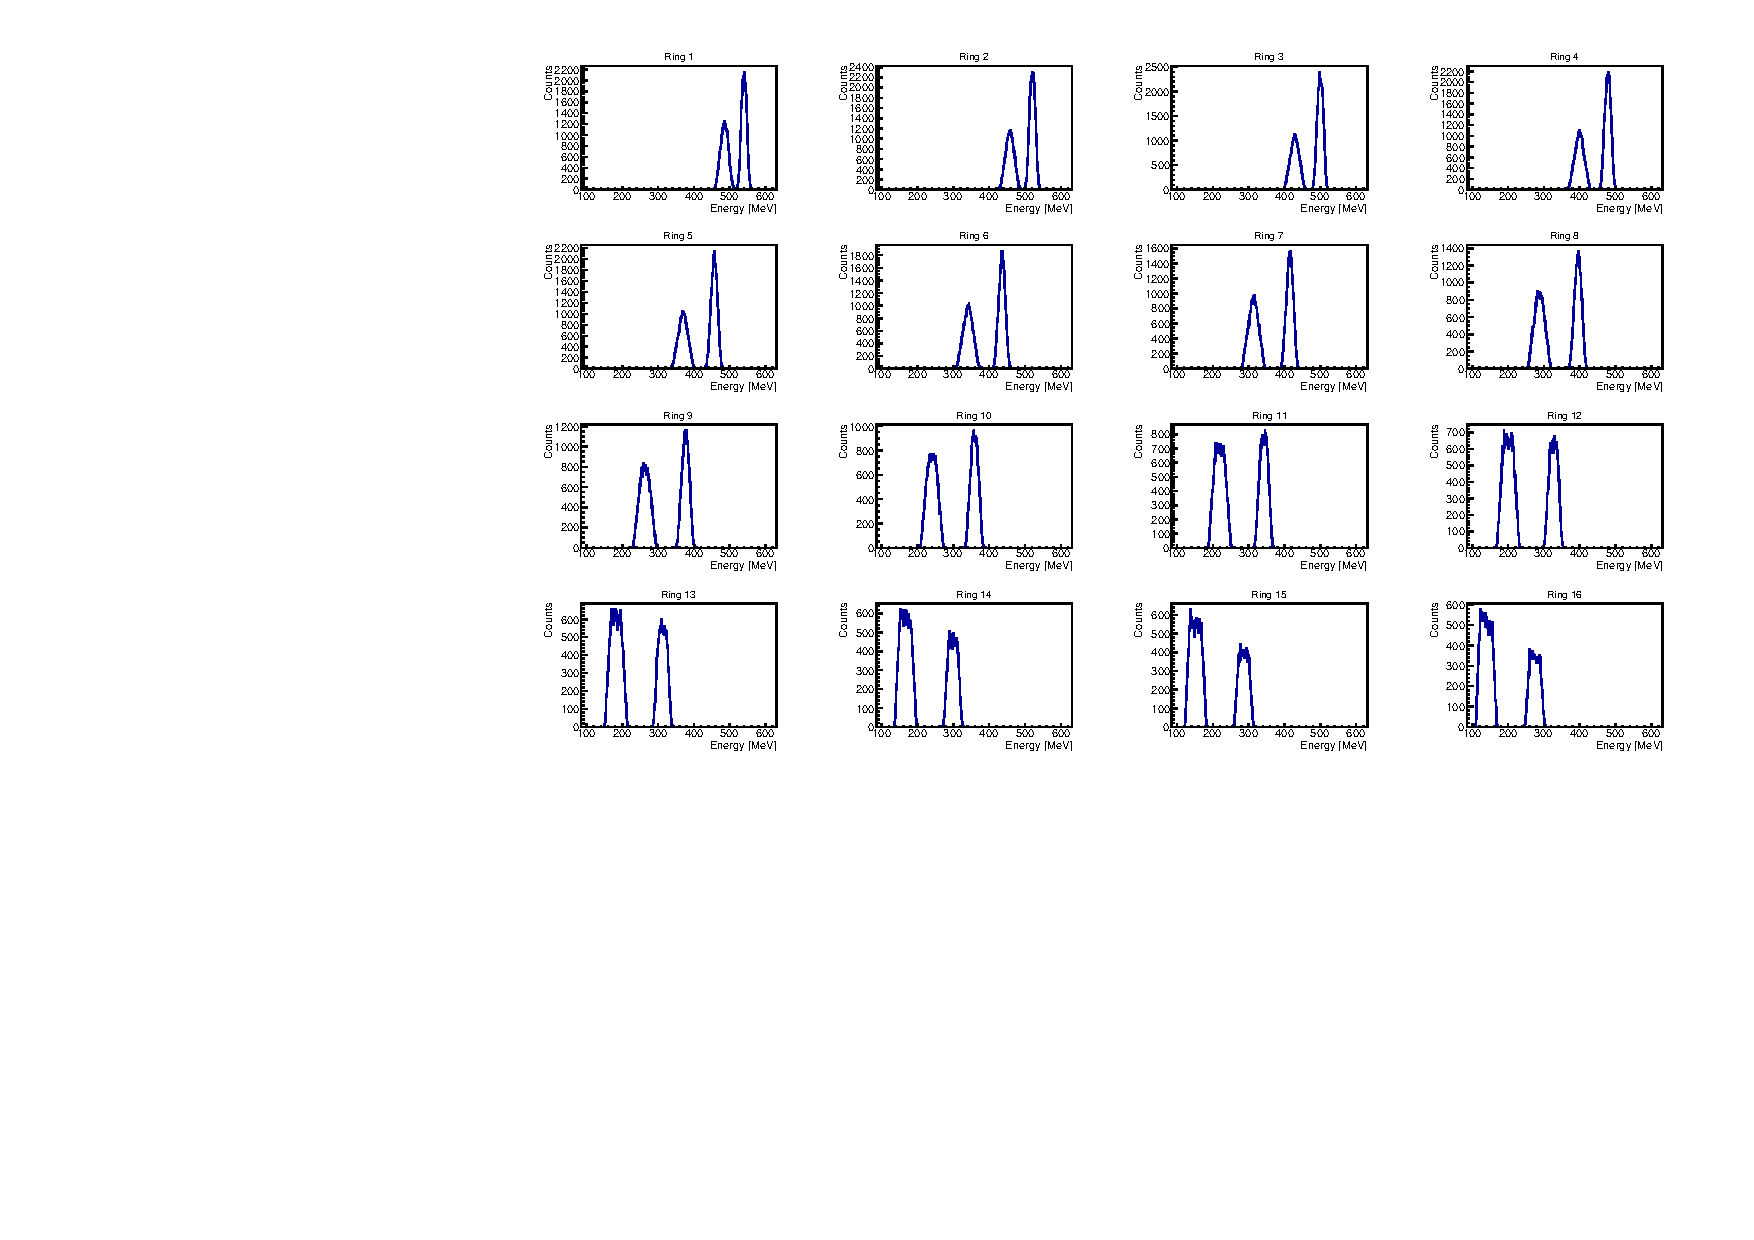
\includepdf[pages={-}, angle=270]{../Plots/simulation/cd_sim_all.pdf}


\end{appendices}



%\bibliographystyle{unsrtnat}
\bibliographystyle{mybibstyle} %my own bibstyle to set first names to one letter + unsrtnat

\bibliography{/Users/trondwj/GitHub/MasterThesis/Thesis/Mendeley/ISOLDE.bib,/Users/trondwj/GitHub/MasterThesis/Thesis/References/web_references.bib}


\end{document}